\chapter[Keramiktechnologie]{Keramiktechnologie}\label{sec:Herstellung}

\begin{multicols}{2}
\raggedcolumns
\noindent Breiter angelegte Studien zur Besiedlung des zentralafrikanischen Regenwaldes durch keramikproduzierende Bevölkerungen legten den Fokus bislang vornehmlich auf die Analyse stilistischer Eigenheiten \parencites[siehe][]{Wotzka.1995}{MbidaMindzie.19951996}{AssokoNdong.20002001}{Clist.20042005}{GouemGouem.20102011}{NlendNlend.20132014}. Die in diesen Arbeiten detailliert ausgeführten formalen Beschreibungen der Artefakte erlauben wenig interpretativen Zugang für eine tiefere Auseinandersetzung mit den Individuen und Gruppen, welche die Untersuchungsmaterialen einst erzeugt haben \parencite[siehe][238\,f.]{vanderLeeuw.1993}. Die hierzu nötige Untersuchung der Keramiktechnologie wurde zwar auch grundsätzlich diskutiert, jedoch nicht systematisiert und auch nicht in die postulierten Modelle integriert.\footnote{Zu neueren Untersuchungen, innerhalb derer entsprechende Fragestellungen bereits einen integralen Bestandteil bilden, siehe \textcite{Riemer.2011} sowie \textcites{Mayor.2011}{Gallay.2012}{vanDoosselaere.2014}.} Eine Studie an Gefäßbeigaben aus den in der Upemba-Senke ergrabenen Gräbern\footnote{Siehe \textcites{deMaret.1977}{deMaret.1999a}{deMaret.2016}.} durch \textcite{LivingstoneSmith.2010c} legt den Fokus auf die Keramiktechnologie und zielt auf eine enge Integration von archäologischen und ethnografischen Quellen zur Töpferei ab. Trotz eines begrenzten Materialkorpus werden die Ähnlichkeiten zwischen den archäologischen und rezenten Töpfereierzeugnissen klar aufgezeigt, was eine skizzenhafte Rekonstruktion des Wissentransfers innerhalb der regionalen Töpferei-Tradition für die letzten sechs Jahrhunderte erlaubt (ebd. 137--140).

Bestimmendes analytisches Konzept zur Untersuchung technologischer Entscheidungsketten innerhalb der Archäologie ist die \textit{\mbox{chaîne} opératoire}\footnote{Im deutschsprachigen Raum findet das Konzept \textit{\mbox{chaîne} opératoire} für die Analyse von Gefäßkeramik bislang kaum Anwendung, anders als innerhalb der frankophonen Archäologie \parencites[siehe][]{Gosselain.1992}{Huysecom.1994}{Visseyrais.2006}{Manem.2008}{Mayor.2011b}{Roux.2011}{Ard.2014}{Gomart.2014}. Generell basieren Studien, die sich mit Töpfereitechnologie beschäftigen, das Konzept \textit{\mbox{chaîne} opératoire} regelhaft als methodischen Rahmen \parencites[siehe][]{vanderLeeuw.1993}{PeuramakiBrown.2004}{Berg.2007}{Berg.2011}{Berg.2017}{DeLaFuente.2011}.}. Konkret beschreibt die \textit{\mbox{chaîne} opératoire} die Abfolge von Entscheidungsgängen, die sich in den zu untersuchenden Quellen materialisiert beziehungsweise aus diesen rekonstruierbar ist.\footnote{Für die Untersuchung von keramischen Inventaren wird grundsätzlich ein \enquote{sequenzieller} Arbeitsablauf empfohlen \parencites[siehe][25; 26 Abb.~4]{Ard.2014}[nach][]{Roux.2007}{Roux.2010}. Dabei bilden Beobachtungen makroskopischer Spuren, die Hinweis auf die Töpferei- beziehungsweise Aufbautechnik liefern, die erste Analyseebene (Kap.~\ref{sec:Herstellung2_Toepferei}). Die sich daraus ergebenden \enquote{technischen Gruppen} (\textsc{Roux} 2010: 7 Abb.\,1) werden in einem nächsten Arbeitsschritt auf petrografische Gemeinsamkeiten und Unterschiede hin untersucht, woraus sich \enquote{technisch-petrografische Gruppen} (ebd.) ergeben (Kap.~\ref{sec:Herstellung2_Fabric}). Die abschließende Gliederungsebene bilden Untersuchungen morphologischer und stilistischer Elemente (Kap.~\ref{sec:Keramiksequenz}).} Sie sind von unbewussten oder zufälligen Ereignissen, denen ein Objekt während seiner Herstellung oder Nutzung ausgesetzt ist, ebenso abzugrenzen wie von taphonomischen Prozessen, also Einflüssen auf ein Objekt, nachdem es aus der Nutzung genommen wurde.\footnote{Erste strukturelle Ansätze finden sich in den Arbeiten von André \textcites{LeroiGourhan.1964}{LeroiGourhan.1965}, Robert \textcites{Cresswell.1983}{Cresswell.1993} und Pierre \textcites{Lemonnier.1992}{Lemonnier.2002}. Die Herausbildung als analytische Methode geht vor allem auf die frankophone Paläolithikumsforschung zurück \parencites{Audouze.2002}[104\,f.]{BarYosef.2009}, und grundsätzlich können auch die auf dem gleichen Grundgedanken aufbauenden, mehr oder weniger parallel entwickelten Konzeptionen \textit{work chain} \parencite{Cresswell.1990} und \textit{operational sequence} \parencites {Perles.1992}{Dibble.1995}{Chazan.2003}[nach][105]{BarYosef.2009} synonym verwendet werden.}

\section{Makrospuren und Herstellungstechniken}\label{sec:Herstellung2_Toepferei}

Die Untersuchung ur- und frühgeschichtlicher Gefäßkeramik unter Berücksichtigung von an den Stücken sichtbaren Makrospuren, welche Hinweis auf die für den Aufbau genutzte Technik geben, wurde anhand einer kleinen, aus 28 Gefäßeinheiten (GE) bestehenden Stichprobe realisiert (Tab.~\ref{tab:Makrospuren_ChaineOperatoire}).\footnote{Die an dieser Stelle zu besprechende Untersuchung wurde erst zu einem sehr späten Stadium der Arbeit als zusätzliche Analyse-Ebene hinzugefügt und konnte daher nicht mehr systematisch alle stilistisch sowie technisch (\textit{Fabrics}) untersuchten GE umfassen. Dies hatte zur Folge, dass nur in begrenztem und sehr konkretem Rahmen Fragestellungen in die Untersuchung einfließen konnten und auch keine generalisierenden Aussagen möglich waren. Die für die Auswahl an GE formulierten Fragen richteten sich an ein Inventar, das durch eine vorangegangene stilistische Analyse (Kap.~\ref{sec:Keramiksequenz}) bereits gegliedert war. Ein systematischer, dem Methodenspektrum der \textit{\mbox{chaîne} opératoire} verhafteter Ansatz \parencite[siehe][25\,f.]{Ard.2014} ließ sich aufgrund des bereits größtenteils abgeschlossenen Zustandes der Arbeit nicht mehr umsetzen.} Ziel der Untersuchung war die Auseinandersetzung mit folgenden Kernfragen:
\begin{itemize*}
	\item Können bereits bei einer kleinen, sich aus stilistisch beschriebenen GE zusammensetzenden Stichprobe Unterschiede in der Herstellungstechnik beobachtet werden?
	\item Lassen sich \textit{Technologietraditionen} identifizieren?
	\item Liefert die Untersuchung von an der Keramik beobachtbaren und auf die Herstellung zurückführbarer Makrospuren einen Beitrag für die Frage der Besiedlungsgeschichte des Arbeitsgebietes?
\end{itemize*}

\noindent Die Auswahl der GE erfolgte mit Bezug auf die genannten Kernfragen nach folgenden Kriterien:
\begin{itemize*}
	\item Die GE sollten möglichst vollständig erhalten sein.
	\item Die sich durch die stilistische Untersuchung (Kap.~\ref{sec:Keramiksequenz}) abzeichnende Sequenz keramischer Stile (Abb.~\ref{fig:Chronologiesystem}) sollte bestmöglich abgedeckt werden.
	\item Die ausgewählten Stilgruppen sollten möglichst durch mehrere GE repräsentiert sein.
\end{itemize*}

\noindent Ein besonderes Augenmerk lag auf der Erschließung von Gemeinsamkeiten wie Unterschieden zwischen den folgenden, durch stilistische Betrachtungen erarbeiteten Gruppen:
\begin{itemize*}
	\item Welche Charakteristika zeigt die im Arbeitsgebiet nur durch wenige GE belegte älteste keramische Stilgruppe des Kongobeckens Imbonga (Kap.~\ref{sec:IMB-Gr})?
	\item Welche Gemeinsamkeiten und Unterschiede ergeben sich zwischen den beiden ältesten keramischen Stilen des Arbeitsgebiets: Batalimo-Maluba (Kap.~\ref{sec:BTM-Gr}) im nördlichen und Pikunda-Munda (Kap.~\ref{sec:PKM-Gr}) im südlichen Teil?
	\item Zeichnet sich die schwache stilistische Variation innerhalb des Pikunda-Munda-Stils (Kap.~\ref{sec:PKM-Gr}) auch auf Ebene der Herstellungstechniken ab?
	\item Welche Gemeinsamkeiten und Unterschiede zeigt das stilistisch nicht mit den übrigen Funden in Einklang zu bringende Fund-Ensemble vom Fundplatz bei Flusskilometer 186 am \mbox{Likwala}-\mbox{aux}-\mbox{Herbes} (Kat.-Nr.~19; Kap.~\ref{sec:SHG-LKW_Einzelfunde})?
	\item Welche Gemeinsamkeiten und Unterschiede ergeben sich zwischen der stilistisch nicht uneingeschränkt an das Material aus dem Inneren Kongobecken anzubindenden Keramik des Pikunda-Munda-Stils (Kap.~\ref{sec:PKM-Gr}) zu den in formaler Hinsicht zweifelsfreie Ähnlichkeiten zeigenden GE des Ngombe-Sils (Kap.~\ref{sec:NGO-Gr})?
	\item Weisen die ältesten Stile im nördlichen Teil des Arbeitsgebietes, Batalimo-Maluba (Kap.~\ref{sec:BTM-Gr}) und \mbox{Ngbanja} (Kap.~\ref{sec:NGB-Gr}), Unterschiede in der Herstellungstechnik auf?
	\item Welche Gemeinsamkeiten und Unterschiede ergeben sich zwischen den entlang des \mbox{Sangha} verbreiteten Stilen Pikunda-Munda (Kap.~\ref{sec:PKM-Gr}), Ngombe (Kap.~\ref{sec:NGO-Gr}), Mandombe (Kap.~\ref{sec:MDB-Gr}) und Konda (Kap.~\ref{sec:KON-Gr})?
	\item Welche Gemeinsamkeiten und Unterschiede ergeben sich zwischen den entlang des Likwala-aux-Herbes vertretenden Stilen Pikunda-Munda (Kap.~\ref{sec:PKM-Gr}), Ebambe (Kap. \ref{sec:EBA-Gr}) und Epena (Kap. \ref{sec:EPE-Gr})?
	\item Welche Gemeinsamkeiten und Unterschiede bestehen zwischen den entlang des \mbox{Ubangi} erfassten Stilen Batalimo-Maluba (Kap.~\ref{sec:BTM-Gr}), \mbox{Ngbanja} (Kap.\ref{sec:NGB-Gr}), Dongo (Kap.~\ref{sec:DON-Gr}) sowie Dama (Kap.~\ref{sec:DAM-Gr}) und Mbati-Ngombe (Kap.~\ref{sec:MBN-Gr})?
\end{itemize*}

\begin{table*}[tb]
	\centering
	\noindent\begin{minipage}[t]{\columnwidth}
{\footnotesize
\begin{sftabular}{@{}lp{.72\columnwidth}l@{}}
\toprule
\textbf{Code} & \textbf{Makro-Spur} & \textbf{Abb.}\\
\midrule
 A1 &  Spur; leicht konkav (evtl. Muschel) & \ref{NGO87-102-28_29_Makrospuren} \\
 A2a &  Spur; fein & \ref{NGB85-101-130-01_Makrospuren} \\
 A2b &  Spur; fein; eng & \ref{MUN87-2-1-1-4-2_Makrospuren} \\
 A3a &  Riefe; horizontal & \\
 A3b &  Riefe; vertikal & \ref{MUN87-1-0-2-6-2_Makrospuren} \\
 A3c &  Riefe; diagonal & \ref{LKW87-186-1_3-13_Makrospuren} \\
 & & \\ 
 B1 &  Eindruck; breit; rund (Stempel) & \\
 B2 &  Eindruck; breit; flach (Spatel/Paddel) & \\
 B3a &  Eindruck; fingerbreit & \\
 B3b &  Eindruck; klein & \ref{MUN87-2-1-1-4-2_Makrospuren} \\
 B4a &  Eindruck; tief (Werkzeugspur) & \ref{MUN87-1-0-2-6-2_Makrospuren} \\
 B4b &  Eindruck; leicht & \\
 & & \\
C1 &  Wandungsdicke; schwankend; vertikal & \ref{ITN87-103_Makrospuren} \\
C2a &  Wandungsdicke; schwankend; horizontal & \ref{MKA87-102-1_Makrospuren} \\
\bottomrule
\end{sftabular}
}
\end{minipage}\hfill
\noindent\begin{minipage}[t]{\columnwidth}
{\footnotesize
\begin{sftabular}{@{}lp{.72\columnwidth}l@{}}
\toprule
\textbf{Code} & \textbf{Makro-Spur} & \textbf{Abb.}\\
\midrule
C2b &  nicht verstrichene Wulst & \ref{DON85-101-71_Makrospuren} \\
C3a &  Wandungsdicke; schwankend (Unebenheit/Buckel) & \ref{MUN87-1-0-2-6-2_Makrospuren} \\
C3b & Wandungsdicke; schwankend; ausgedünnt & \\
C4 &  Absatz im Profil; horizontal & \\
 & & \\
D1a &  Bruch; lagiger Aufbau \parencite[siehe][140 Abb. 8.c]{Lindahl.2010} & \\
D1b & Bruch; diagonal verlaufender Aufbau \parencite[siehe][140 Abb.~8.b]{Lindahl.2010} & \\
D2a &  Bruchlinie; horizontal & \\
D2b &  Bruchlinie; diagonal & \\
D3a &  Riss; fein; horizontal & \ref{NGO87-102-27_Makrospuren} \\
D3b &  Riss; fein; spiralig aufsteigend & \ref{LKW87-186-1_3-13_Makrospuren} \\
D3c &  Riss; fein; radial & \ref{MUN87-1-0-2-1-3_Makrospuren} \\
D3d &  Riss; fein; vertikal & \ref{MIT87-103-1_Makrospuren} \\
\bottomrule
\end{sftabular}
}
\end{minipage}
	\caption{Makro-Spuren: An den GE beobachtete Spuren.}
	\label{tab:Makrospuren_Liste}
\end{table*}

\vspace{1.5em}
\noindent Die zur weiteren Begutachtung ausgewählten 28~GE spiegeln zwölf verschiedene keramische Stilgruppen wider.\footnote{In alphabetischer Reihenfolge sind die folgenden Stilgruppen vertreten: 1~GE der Batalimo-Maluba-Gruppe (Kap.~\ref{sec:BTM-Gr}; BTM, 4~GE der Dama-Gruppe (Kap.~\ref{sec:DAM-Gr}; DAM), 1~GE der Dongo-Gruppe (Kap.~\ref{sec:DON-Gr}; DON), 3~GE der Ebambe-Gruppe (Kap.~\ref{sec:EBA-Gr}; EBA), 2~GE der Epena-Gruppe (Kap.~\ref{sec:EPE-Gr}; EPE), 2~GE der Imbonga-Gruppe (Kap.~\ref{sec:IMB-Gr}; IMB), 2~GE der Konda-Gruppe (Kap.~\ref{sec:KON-Gr}; KON), 1~GE vom Fundplatz \mbox{Likwala}-\mbox{aux}-\mbox{Herbes} Flusskilometer 186 (LKW), 2~GE der Mandombe-Gruppe (Kap.~\ref{sec:MDB-Gr}; MDB), 2~GE der Ngbanaja-Gruppe (Kap.~\ref{sec:NGB-Gr}; NGB), 2~GE der Ngombe-Gruppe (Kap.~\ref{sec:NGO-Gr}; NGO) und 6~GE der Pikunda-Munda-Gruppe (Kap.~\ref{sec:PKM-Gr}; PKM). Die genannten Stilgruppenkürzel finden sich in Tab.~\ref{tab:Makrospuren_ChaineOperatoire} wieder.\label{ftn:StilGrKurzel_UntersuchungHerstetellungstechnik}} An den in der Stichprobe enthaltenen GE konnten insgesamt 27 verschiedene Makrospuren unterschieden werden, die im Zusammenhang mit der Herstellung der Gefäße stehen (Tab.~\ref{tab:Makrospuren_Liste}). Eine systematische Aufnahme der Spuren für jede GE orientierte sich an der in dieser Arbeit genutzten Bereichs-Aufteilung für Verzierungselemente (siehe Abb.~\ref{fig:Keramik_VerzZonen}). Die beobachteten Makrospuren wurden in vier größere Gruppen unterschieden (Tab.~\ref{tab:Makrospuren_Liste}): A) Spuren, die durch Kratzen oder Schaben mit einem Werkzeug erzeugt wurden, B) Spuren, die durch das Eindrücken mit einem Werkzeug entstanden sind, C) Schwankungen der Wandung eines Gefäßes und D) Eigenschaften der Brüche. Die Spuren der ersten beiden Gruppen sind am häufigsten zu beobachten, repräsentieren jedoch vornehmlich die abschließende Behandlung der Oberflächen eines Gefäßes. Die Spuren der Gruppen C und D ließen sich seltener beobachten, geben jedoch Hinweise auf den internen Aufbau eines Gefäßes und damit die genutzte Herstellungs- beziehungsweise Gefäßaufbautechnik.

\begin{figure*}[p]
	\centering
	\begin{subfigure}{\textwidth}
		\centering
		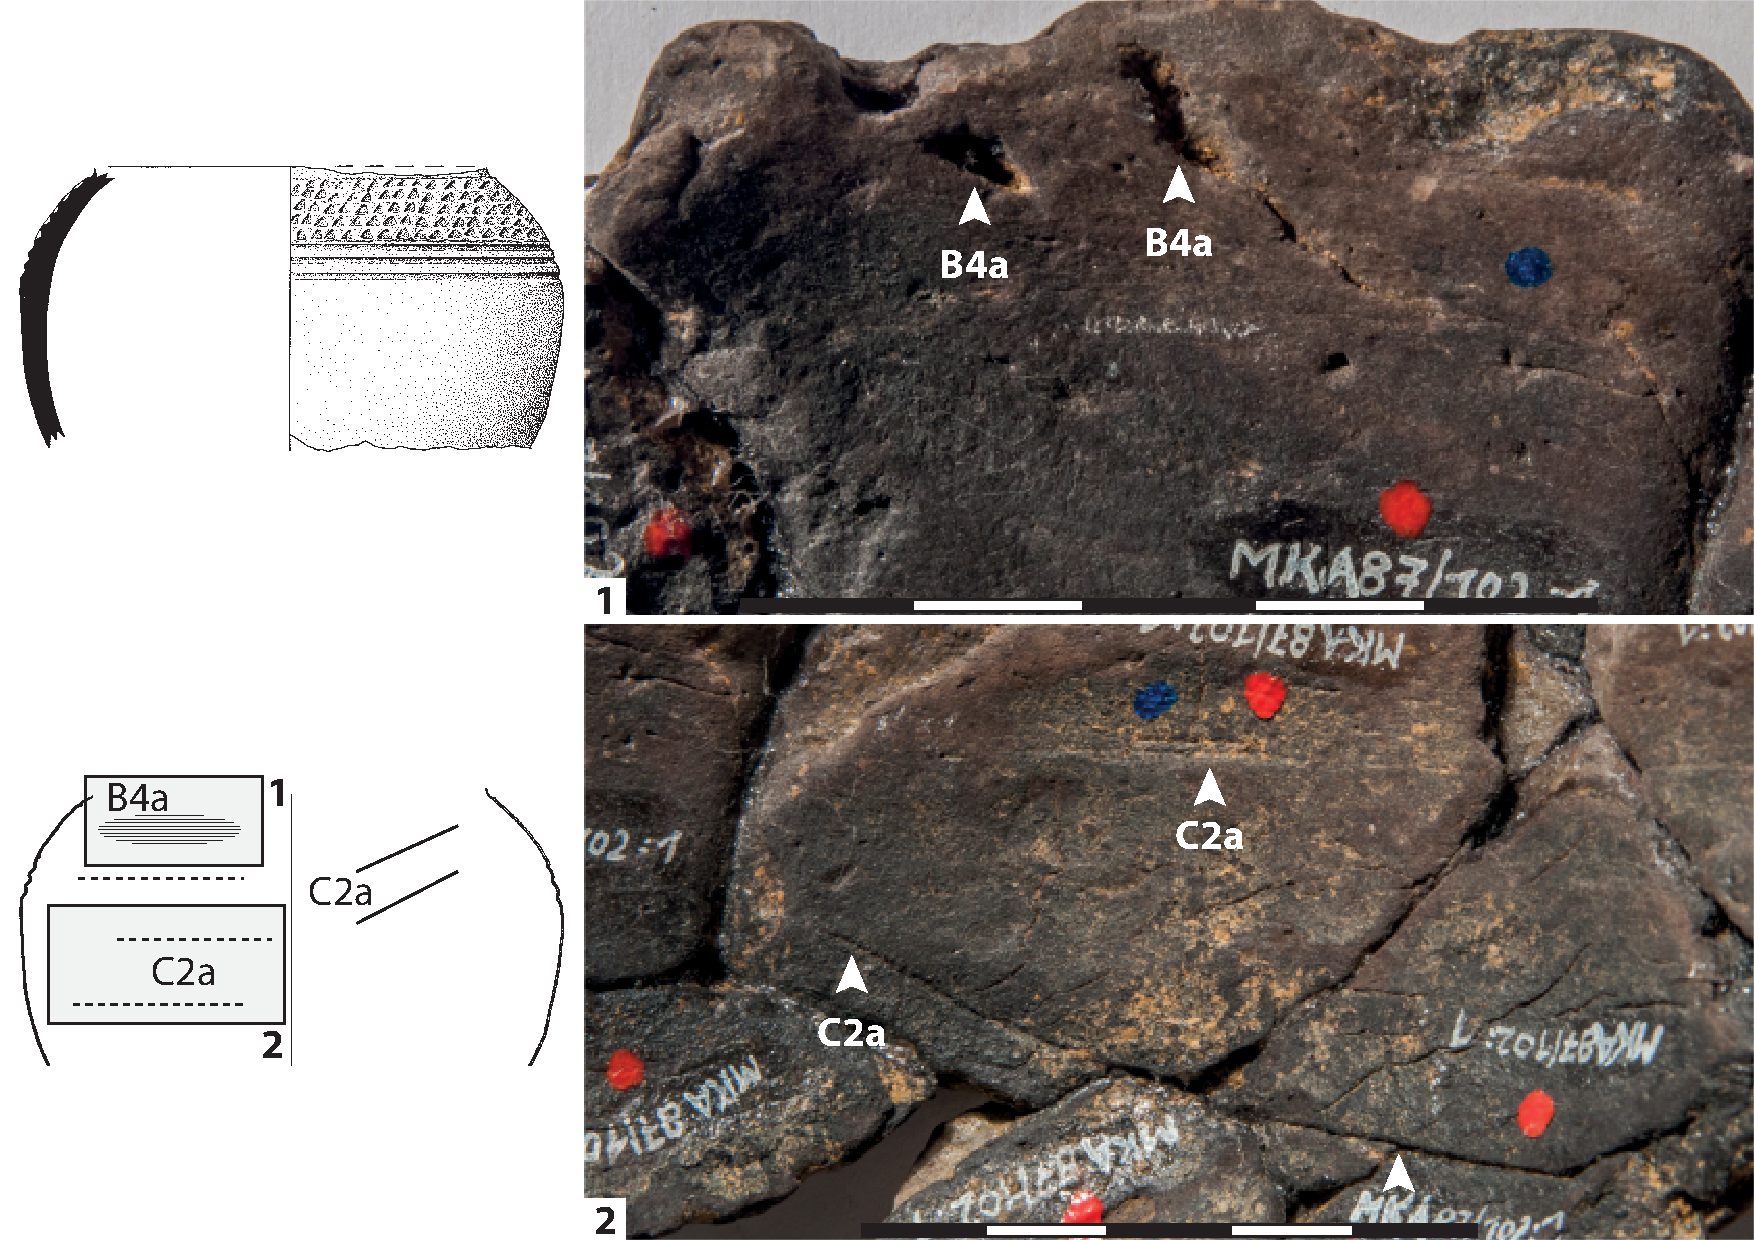
\includegraphics[width = \textwidth]{fig/Abb_Macrotraces/MKA87-102-1.pdf}
		\caption{Mobaka (Fpl.~246): Obj.~MKA~87/102:1 (Taf.~39.5).\vspace{1em}}
		\label{MKA87-102-1_Makrospuren}
	\end{subfigure}
	\begin{subfigure}{\textwidth}
		\centering
		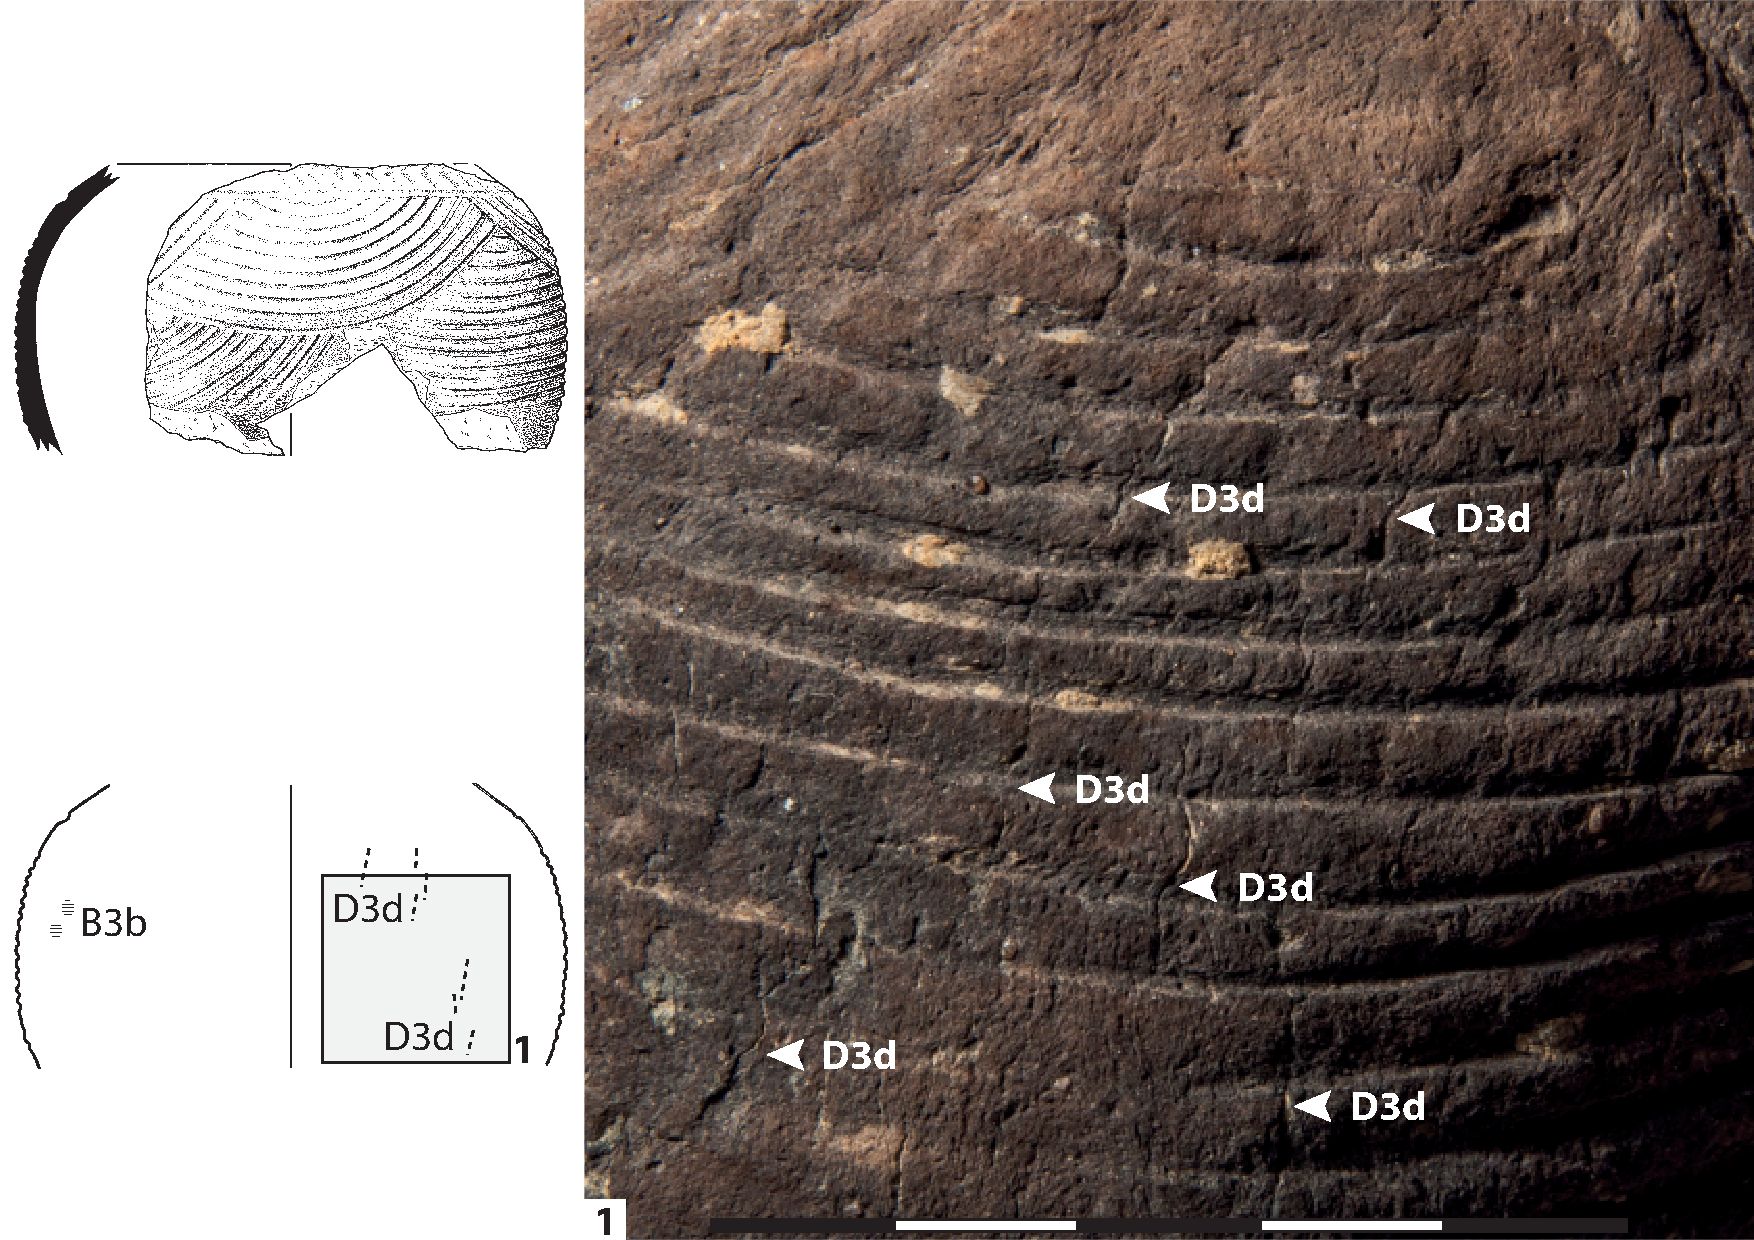
\includegraphics[width = \textwidth]{fig/Abb_Macrotraces/MIT87-103-1.pdf}
		\caption{Mitula (Fpl.~251): Obj.~MIT~87/103:1 (Taf.~42.10).}
		\label{MIT87-103-1_Makrospuren}
	\end{subfigure}
	\caption{Makrospuren: Aufnahme und Details.}
\end{figure*}

Stellvertretend für die ältesten im Arbeitsgebiet vertretenen Stilgruppen wurden Stücke aus ausgegrabenen und gut datierten Komplexen ausgewählt. Die beiden der Imbonga-Gruppe (Kap. \ref{sec:IMB-Gr}) zuweisbaren Stücke aus Mobaka und Mitula liefern einen ersten Einblick in die mit den Herstellungsprozessen in Zusammenhang stehenden Makrospuren dieser vor allem weiter östlich verbreiteten, frühesten Keramik der Region. An der Außenseite des Gefäßes aus Mobaka (Abb.~\ref{MKA87-102-1_Makrospuren}) finden sich im Bereich der größten Weite flache, diagonal aufsteigende rippenartige Erhebungen, die zu einer schwankenden Wandungsdicke führen (C2a). An der Innenseite lassen sich im Bereich des Gefäßbauches horizontale, flache Verdickungen und Eintiefungen beobachten, die ebenfalls zu Schwankungen der Wandungsstärke entlang des Profils führen (Abb.~\ref{MKA87-102-1_Makrospuren}.2:~C2a). Unterhalb des Schulter-Umbruches befinden sich bis auf etwa die halbe Wandungsdicke reichende Eintiefungen (Abb.~\ref{MKA87-102-1_Makrospuren}.1:~B4a), die möglicherweise auf die Verbindung separat gefertigter Teile hinweisen. Die Brüche lassen eine plattige beziehungsweise parallel zur Wandung verlaufende Struktur erkennen (D1a), die auf einen Aufbau durch Treiben hindeutet \parencite[140 Abb. 8.c--d]{Lindahl.2010}. Die Außenseite des Gefäßes aus Mitula weist einige feine, vertikal verlaufende Bündel aus Rissen auf (Abb.~\ref{MIT87-103-1_Makrospuren}.1:~D3d). An der Innenseite sind neben vereinzelten leicht inselartigen Erhebungen und Eintiefungen keine Makrospuren zu erfassen. 

\begin{figure*}[p]
	\centering
	\begin{subfigure}{\textwidth}
		\centering
		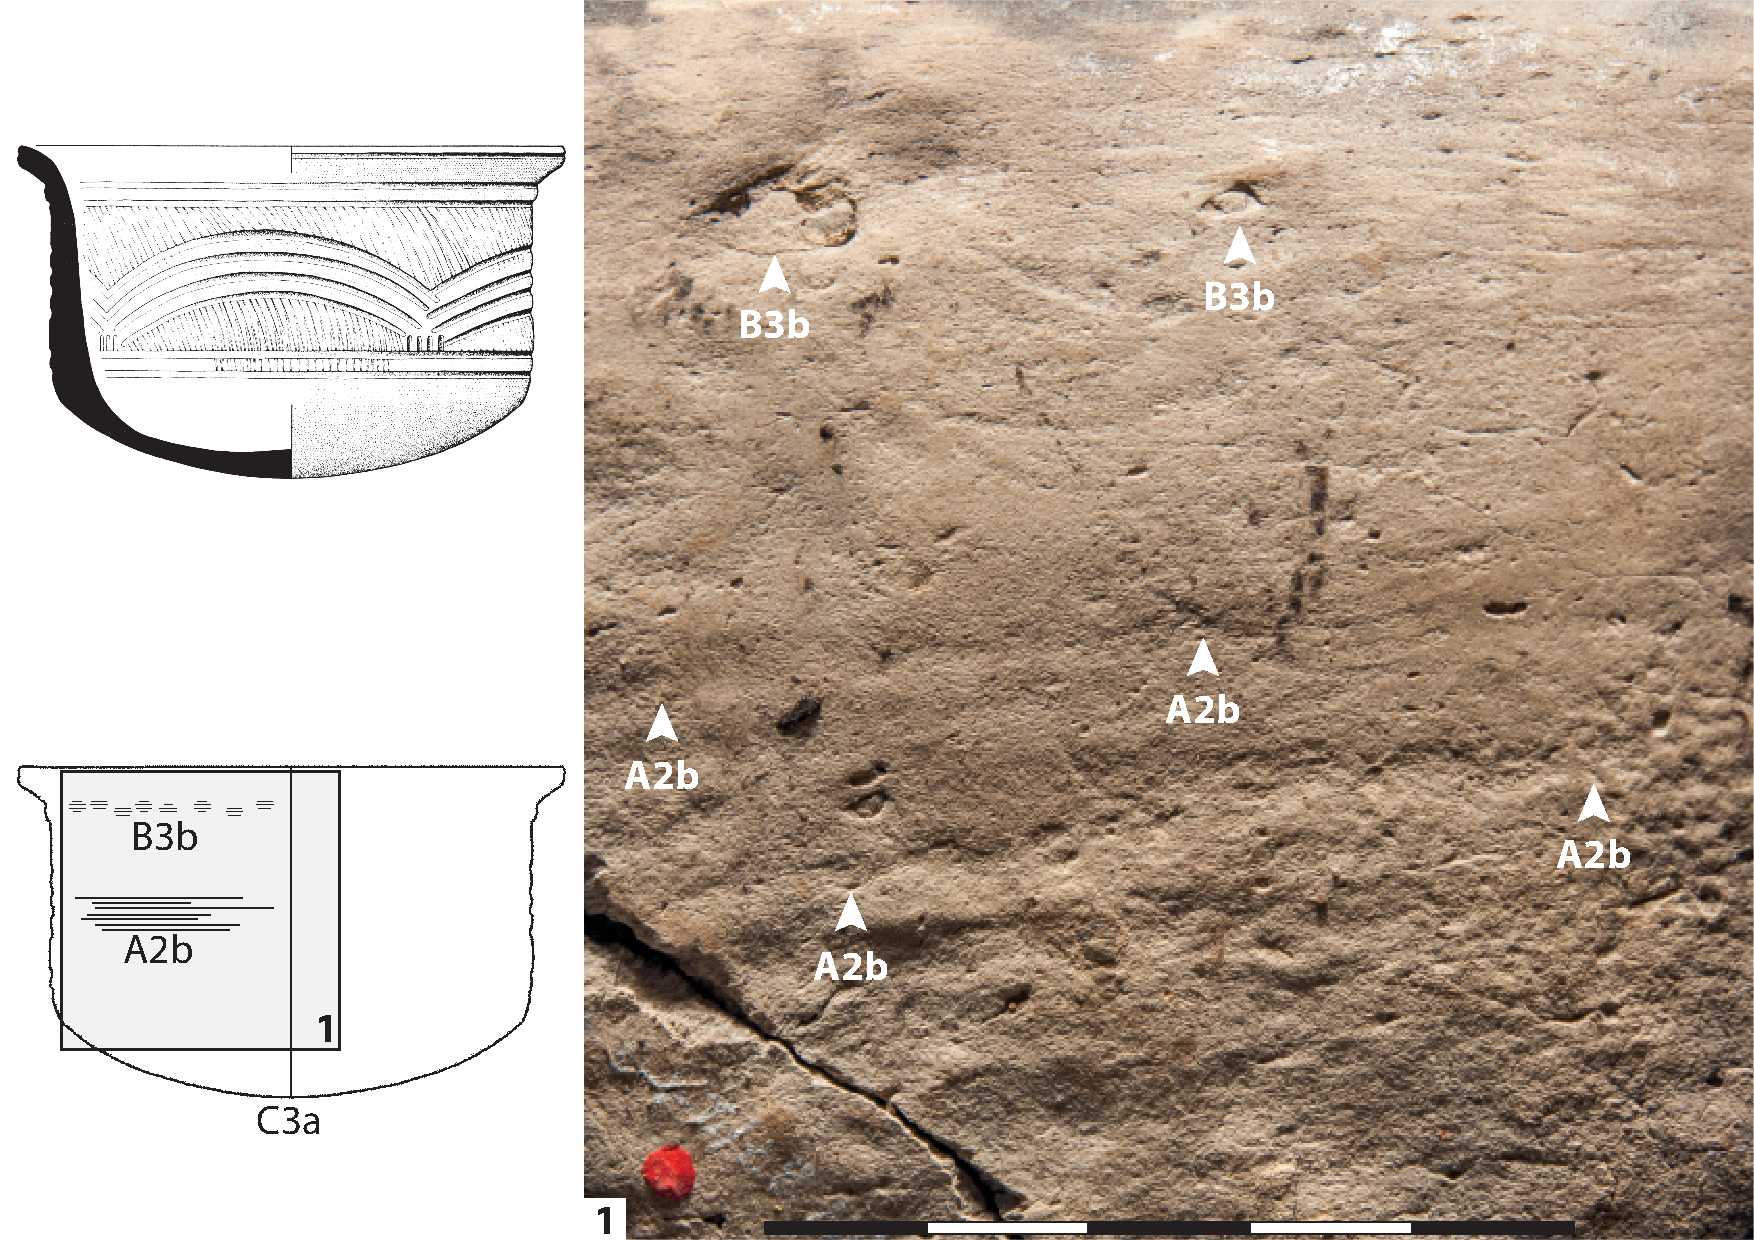
\includegraphics[width = \textwidth]{fig/Abb_Macrotraces/MUN87-2-1-1-4-2.pdf}
		\caption{Munda (Fpl.~304): Obj.~MUN~87/2-1-1-4:2 (Taf.~91.1).\vspace{1em}}
		\label{MUN87-2-1-1-4-2_Makrospuren}
	\end{subfigure}
	\begin{subfigure}{\textwidth}
		\centering
		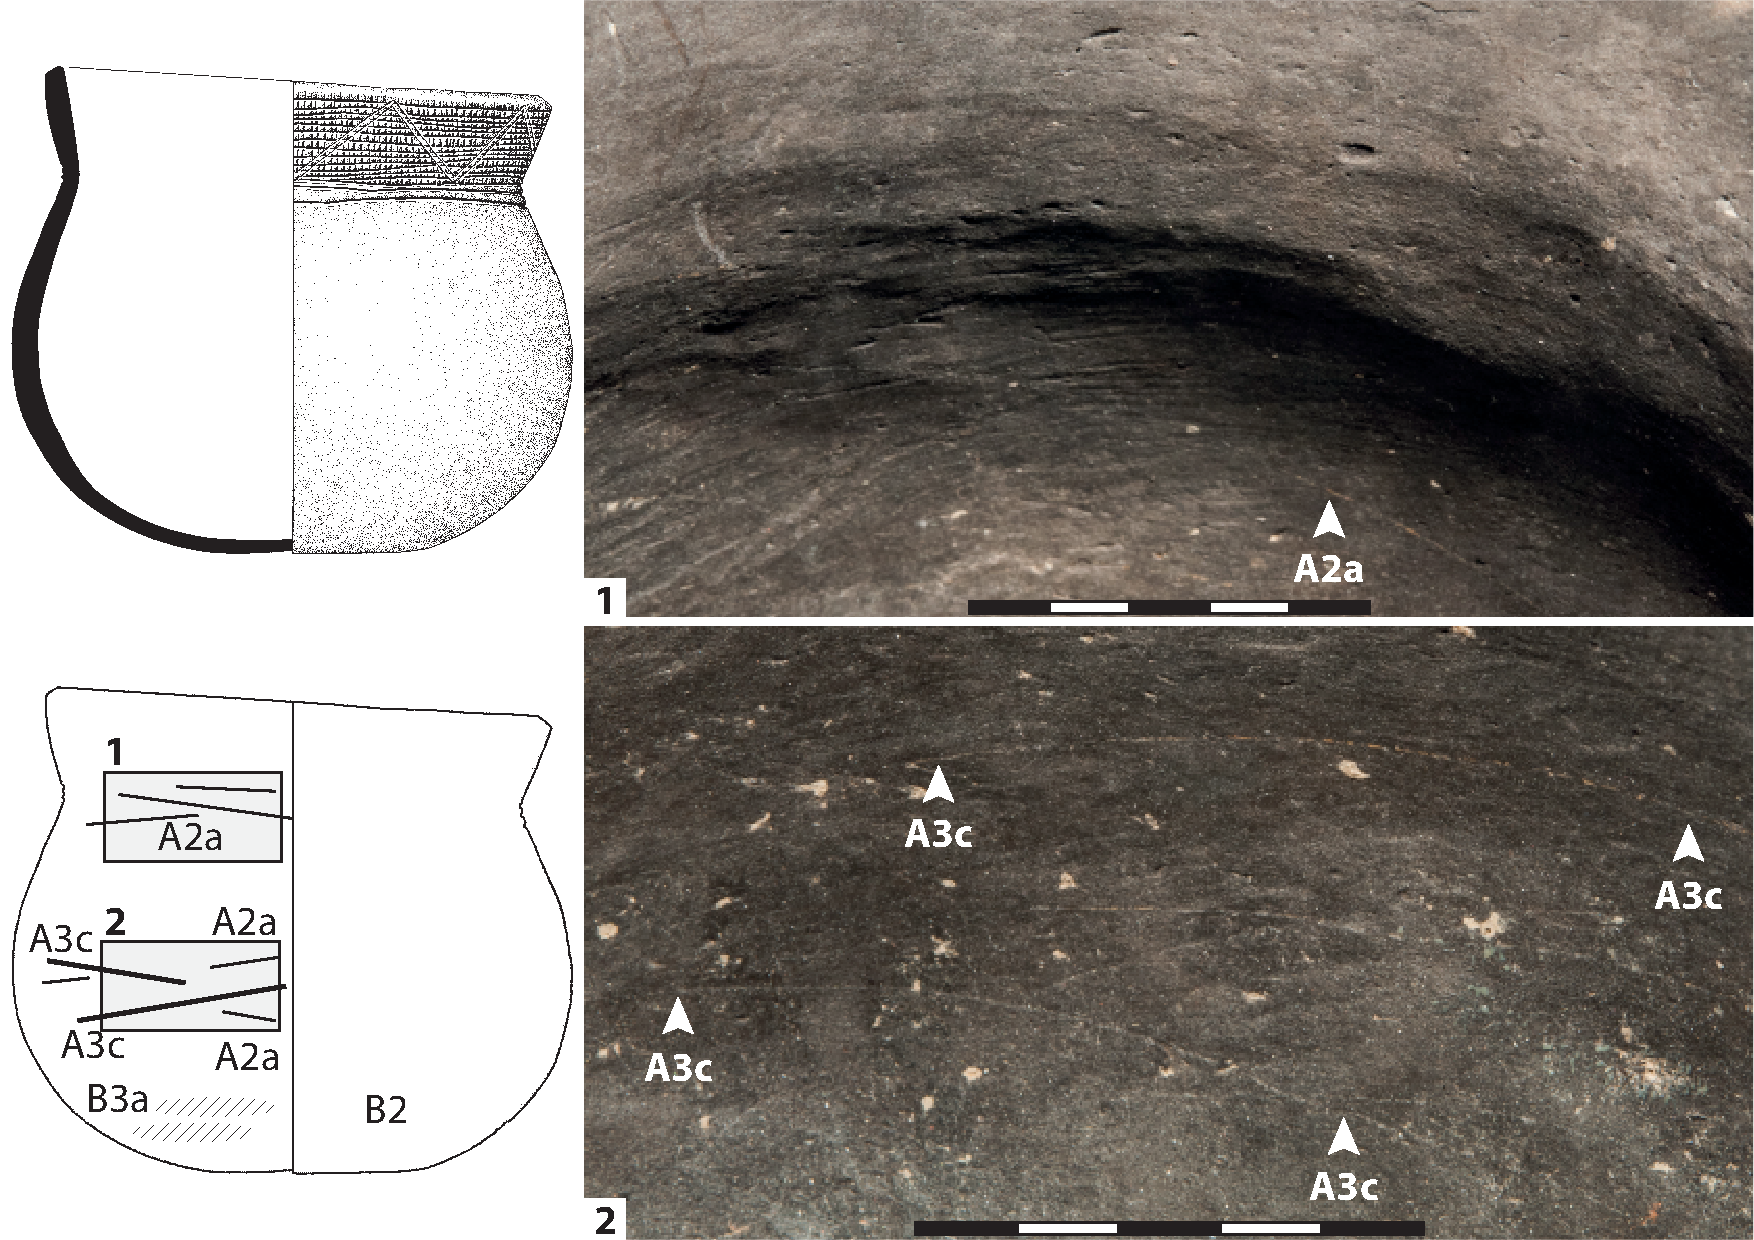
\includegraphics[width = \textwidth]{fig/Abb_Macrotraces/MUN87-2-1-3-10_Gef10.pdf}
		\caption{Munda (Fpl.~304): Obj.~MUN~87/2-1-3:10 (Taf.~93.3).}
		\label{MUN87-2-1-3-10_Makrospuren}
	\end{subfigure}
	\caption{Makrospuren: Aufnahme und Details.}
\end{figure*}

\begin{figure*}[p]
	\centering
	\begin{subfigure}{\textwidth}
		\centering
		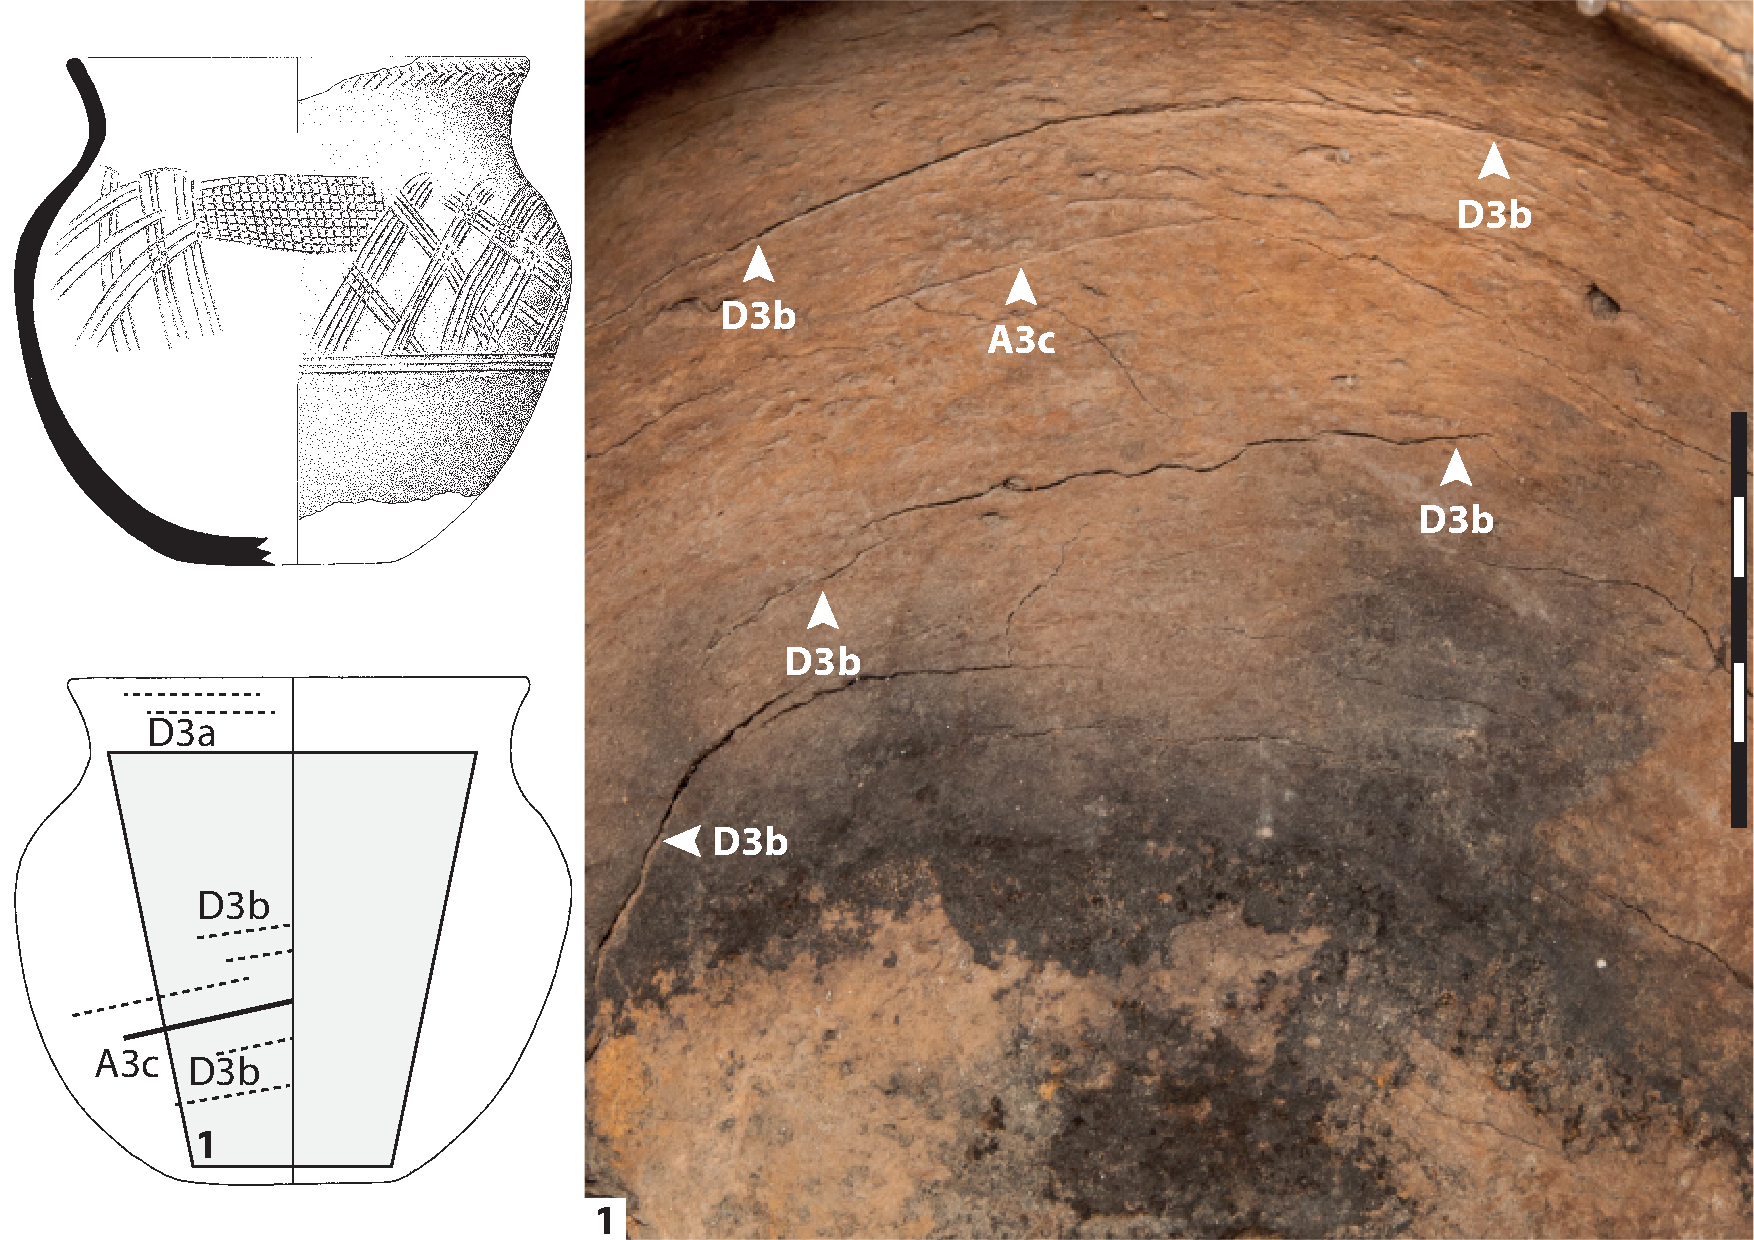
\includegraphics[width = \textwidth]{fig/Abb_Macrotraces/LKW87-186-1_3-13.pdf}
		\caption{Likwala-aux-Herbes, Flusskilometer 186 (Fpl.~291): Obj.~LKW~87/186-1:3--13 (Taf.~76.1).\vspace{1em}}
		\label{LKW87-186-1_3-13_Makrospuren}
	\end{subfigure}
	\begin{subfigure}{\textwidth}
		\centering
		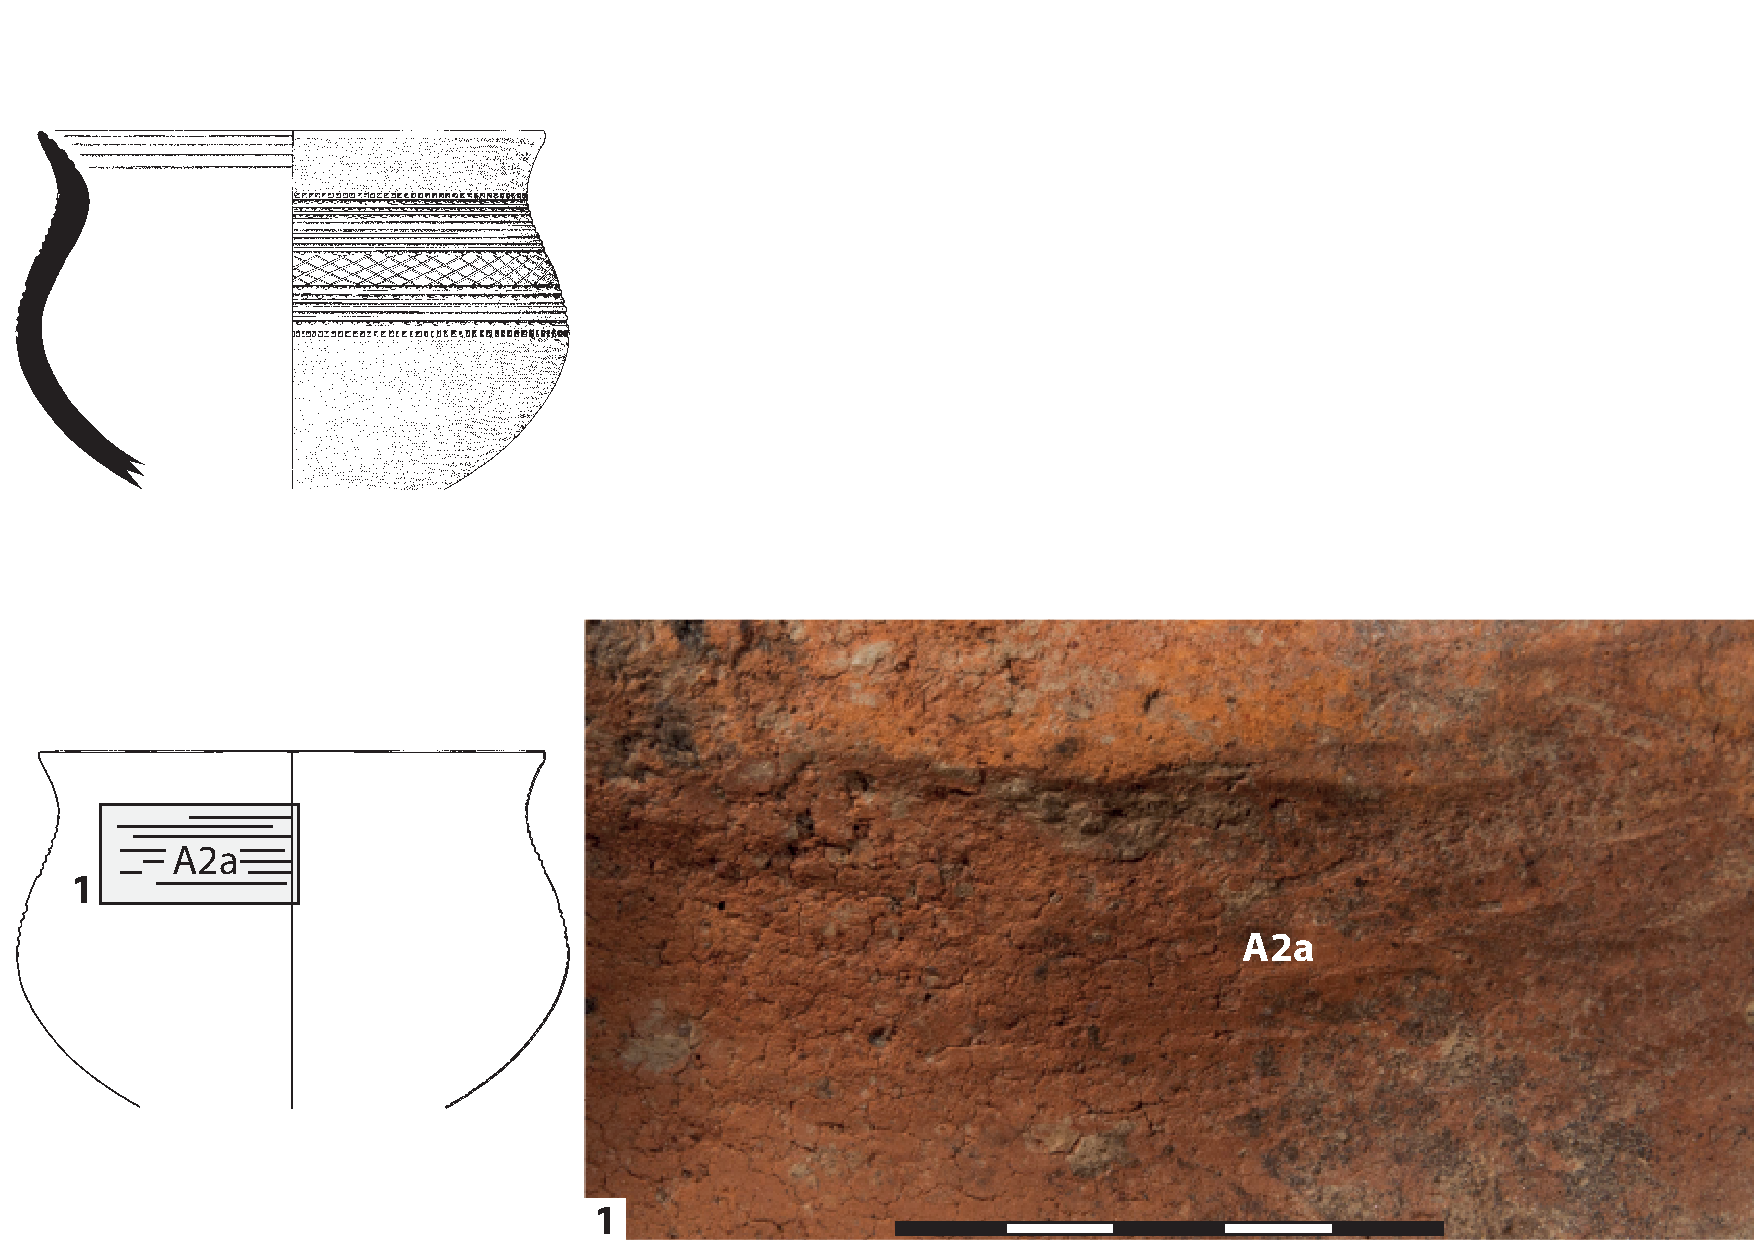
\includegraphics[width = \textwidth]{fig/Abb_Macrotraces/NGB85-101-130.pdf}
		\caption{\mbox{Ngbanja} (Fpl.~199): Obj.~NGB~85/101:131 (Taf.~7.6).}
		\label{NGB85-101-130-01_Makrospuren}
	\end{subfigure}
	\caption{Makrospuren: Aufnahme und Details.}
\end{figure*}

Zwei Gefäße aus dem in Pikunda am mittleren \mbox{Sangha} ausgegrabenen Befund PIK~87/1 (Kat.-Nr.~8) und je zwei weitere Gefäße aus den in Munda am oberen \mbox{Likwala}-\mbox{aux}-\mbox{Herbes} ergrabenen Gruben MUN~87/2-1-1 (Kat.-Nr.~16) sowie MUN~87/2-1-3 (Kat.-Nr.~17) stehen stellvertretend für das Formenspektrum der Pikunda-Munda-Gruppe (Kap.~\ref{sec:PKM-Gr}). Aufgrund seiner flächigen Verzierung lassen sich an der Außenseite eines aus dem Befund PIK~87/1 in Pikunda am \mbox{Sangha} stammenden Gefäßes der Pikunda-Munda-Gruppe (Kat.-Nr.~8; Taf.~44.3) keine Makrospuren erkennen. An der Innenseite weist das Gefäß im oberen Teil lediglich sehr feine, etwa nur 5\,mm voneinander entfernt sitzende Glättspuren (A2b) auf, während der untere Teil feine spiralig beziehungsweise diagonal aufsteigende Risse zeigt (D3b; siehe Abb.~\ref{LKW87-186-1_3-13_Makrospuren}). Die Bruchlinien der einzelnen Fragmente verlaufen vorwiegend diagonal und folgen den feinen Rissen (D2b). Im Bereich des rund ausgeführten Gefäßbodens ließen sich keine Makrospuren beobachten. Die Bruchstruktur des Gefäßes ist bis knapp unterhalb des Randes plattig beziehungsweise parallel zur Wandung (D1a; siehe ebd. 140 Abb. 8.c--d). Eine entsprechende interne Strukturierung kann als Hinweis auf eine Herstellung durch Treiben angesehen werden. Im Randbereich hingegen verläuft die innere Struktur des Scherbens eher diagonal und deutet auf eine Aufbautechnik hin (D1b; ebd. 140 Abb. 8.b). Ein aus mehreren Fragmenten zusammensetzbares, ebenfalls aus dem Befund in Pikunda stammendes Gefäß (Taf.~45.1) weist eine vollständig geglättete Oberfläche auf, die keine Makrospuren zeigt. Im Schulterbereich ist eine leichte Verdickung der Wandung zu beobachten und das einzige auffällige Merkmal ist die Strukturierung der Brüche. Das Gefäß zeigt diagonale Bruch-Facetten (D2d) und innerhalb der Bruchflächen lässt sich ebenfalls eine diagonale Strukturierung erkennen (D1b). Eine der Pikunda-Munda-Schalen aus dem Befund MUN~87/2-1-1 in Munda am \mbox{Likwala}-\mbox{aux}-\mbox{Herbes} (Kat.-Nr.~16) weist unterhalb des Randes eine mehr oder weniger horizontale Reihe kleiner runder bis leicht ovaler Löcher beziehungsweise Eindrücke auf (Abb.~\ref{MUN87-2-1-1-4-2_Makrospuren}.1:~B3b). Die Innenseite der Wandung zeigt vereinzelt eng beieinander sitzende Glättspuren (Abb.~\ref{MUN87-2-1-1-4-2_Makrospuren}.1:~A2b), und der für die Schalen der Pikunda-Munda-Gruppe so charakteristische Profilknick zwischen Wandung und Boden weist im Bruch eine zusätzlich aufgebrachte Wulst auf. Höchstwahrscheinlich markiert der Knick einen Wechsel in der Aufbautechnik. Der rund ausgeführte Boden ist mittig auffällig verdickt (C3a), was auf überschüssiges Material beim möglicherweise finalen Verschließen der Bodenpartie hinweisen kann. Die Innenseite eines zweiten Gefäßes (Taf.~91.5) zeigt ebenfalls flächige, eng beieinander sitzende, feine Glättspuren (A2b). Der Boden hingegen ist glatt und mittig ebenfalls leicht verdickt (C3a). Überdies zeigen sich im Bodenbereich sternförmig zum Zentrum zulaufende Risse (D3c). Zusammengenommen deuten diese Merkmale an, dass der Gefäßboden erst zum Ende des Formgebungsprozesses geschlossen wurde. Im Bruch lässt sich eine plattige, parallel zur Wandung verlaufende Struktur des Scherbens (D1a) beobachten, die als Anzeige für einen Aufbau durch Treiben angesehen werden kann (ebd. 140 Abb. 8.c--d). Ein Gefäß mit geschweifter Wandung und ausbiegendem Rand aus der benachbarten Grube MUN~87/2-1-3 (Kat.-Nr.~17) zeigt im unteren Bereich Wurzelfraß an seiner Außenseite. Auffällig ist eine leichte Facettierung des Gefäßunterteils (B2), die eine Formgebung unter Zuhilfenahme eines Töpferpaddels möglich erscheinen lässt. Die Wandungsdicke im Bereich des rund ausgeführten Bodens ist teilweise deutlich ausgedünnt (C3b), was ebenfalls als Hinweis darauf gewertet werden kann, dass der Boden erst gegen Ende der Formgebung geschlossen wurde, wobei nicht ausreichend Material zur Verfügung stand. An der Innenseite befinden sich im Bereich des Halsansatzes leicht diagonale bis horizontale feine Glättspuren (Abb.~\ref{MUN87-2-1-3-10_Makrospuren}.1:~A2a). Im Bereich des größten Umfangs sind innen bogenförmige, mehr oder minder horizontal verlaufende feine Glättrillen zu sehen (Abb.~\ref{MUN87-2-1-3-10_Makrospuren}.2:~A3c). Ebenfalls fallen in diesem Bereich leichte, spiralig aufsteigende Absätze auf (C2a). Im Bereich des Gefäßbodens befinden sich innen etwa fingerbreite leichte Eindrücke (B3a), die -- wie auch im Fall der Außenseite -- zu einer leichten Facettierung führen. Ein zweites Gefäß, eine der klassischen Pikunda-Munda-Schalen aus dem selben Befund, weist ebenfalls eine stark angelöste und erodierte Oberfläche auf (Taf.~93.1). Nur noch an wenigen Stellen sind Makrospuren sichtbar. Im oberen Gefäßteil befinden sich innen sehr feine und eng sitzende Glättspuren (A2b). Im unteren Gefäßteil beziehungsweise am Bodenansatz schwankt die Wandungsdicke leicht; es bilden sich leicht erhabene und eingetiefte Zonen aus (C2a). Die Wandungsdicke im Bodenbereich ist auffällig gering (C3b). Dies kann darauf hindeuten, dass der Boden ebenfalls erst am Ende geschlossen wurde.

Ein Gefäß aus dem am Flusskilometer 186 am \mbox{Likwala}-\mbox{aux}-\mbox{Herbes} erfassten Grubeninventar (Kat.-Nr.~19) zeigt im Randbereich feine, horizontale Glättspuren (A2) und Risse (Abb.~\ref{LKW87-186-1_3-13_Makrospuren}.1:~D3a). Den gesamten Gefäßbauch durchziehen innen spiralig aufsteigende, lange und tiefe Risse (Abb.~\ref{LKW87-186-1_3-13_Makrospuren}.1:~D3b). In gleicher Orientierung lassen sich auch einige Glättriefen (Abb.~\ref{LKW87-186-1_3-13_Makrospuren}.1:~A3c) beobachten. 

\begin{figure*}[p]
	\centering
	\begin{subfigure}{\textwidth}
		\centering
		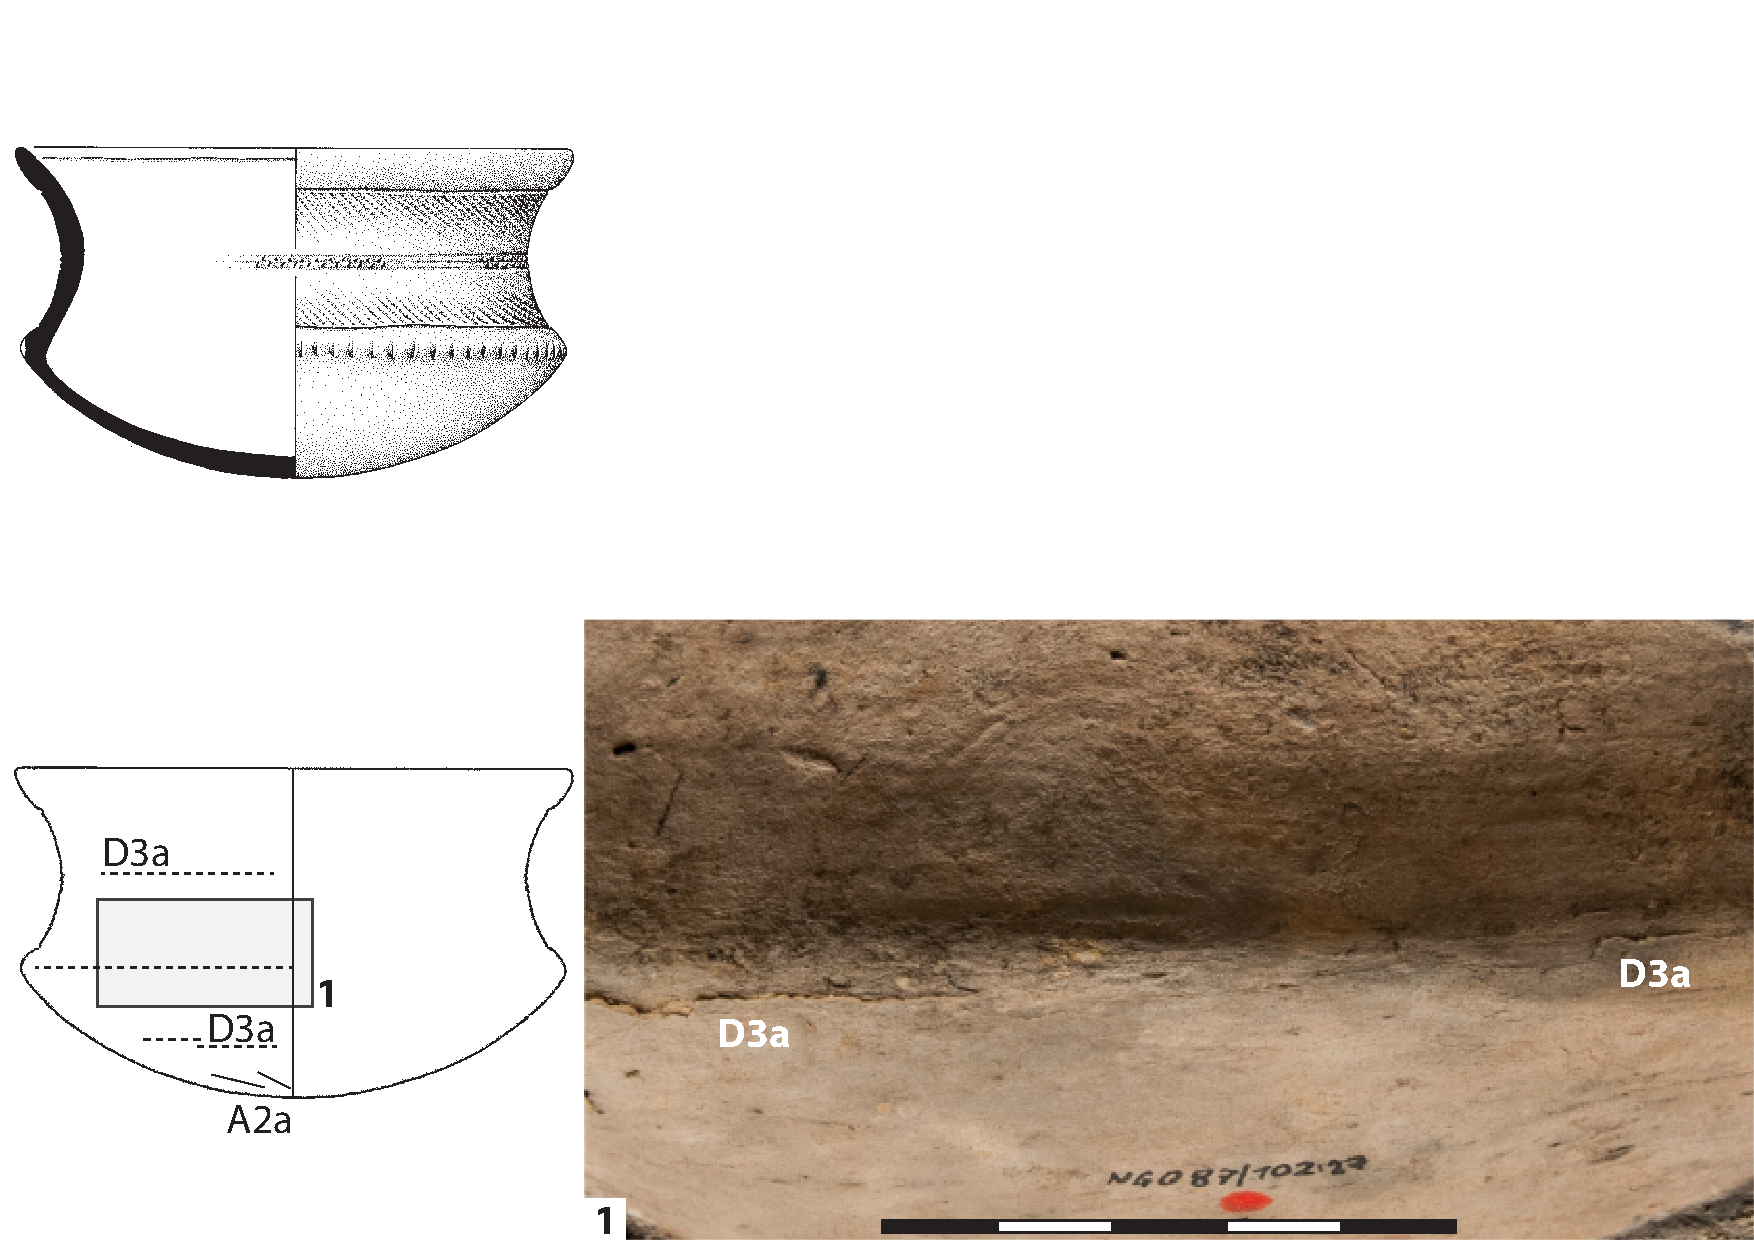
\includegraphics[width = \textwidth]{fig/Abb_Macrotraces/NGO87-102-27.pdf}
		\caption{Ngombe (Fpl.~252): Obj.~NGO~87/102:27 (Taf.~42.16).\vspace{1em}}
		\label{NGO87-102-27_Makrospuren}
	\end{subfigure}
	\begin{subfigure}{\textwidth}
		\centering
		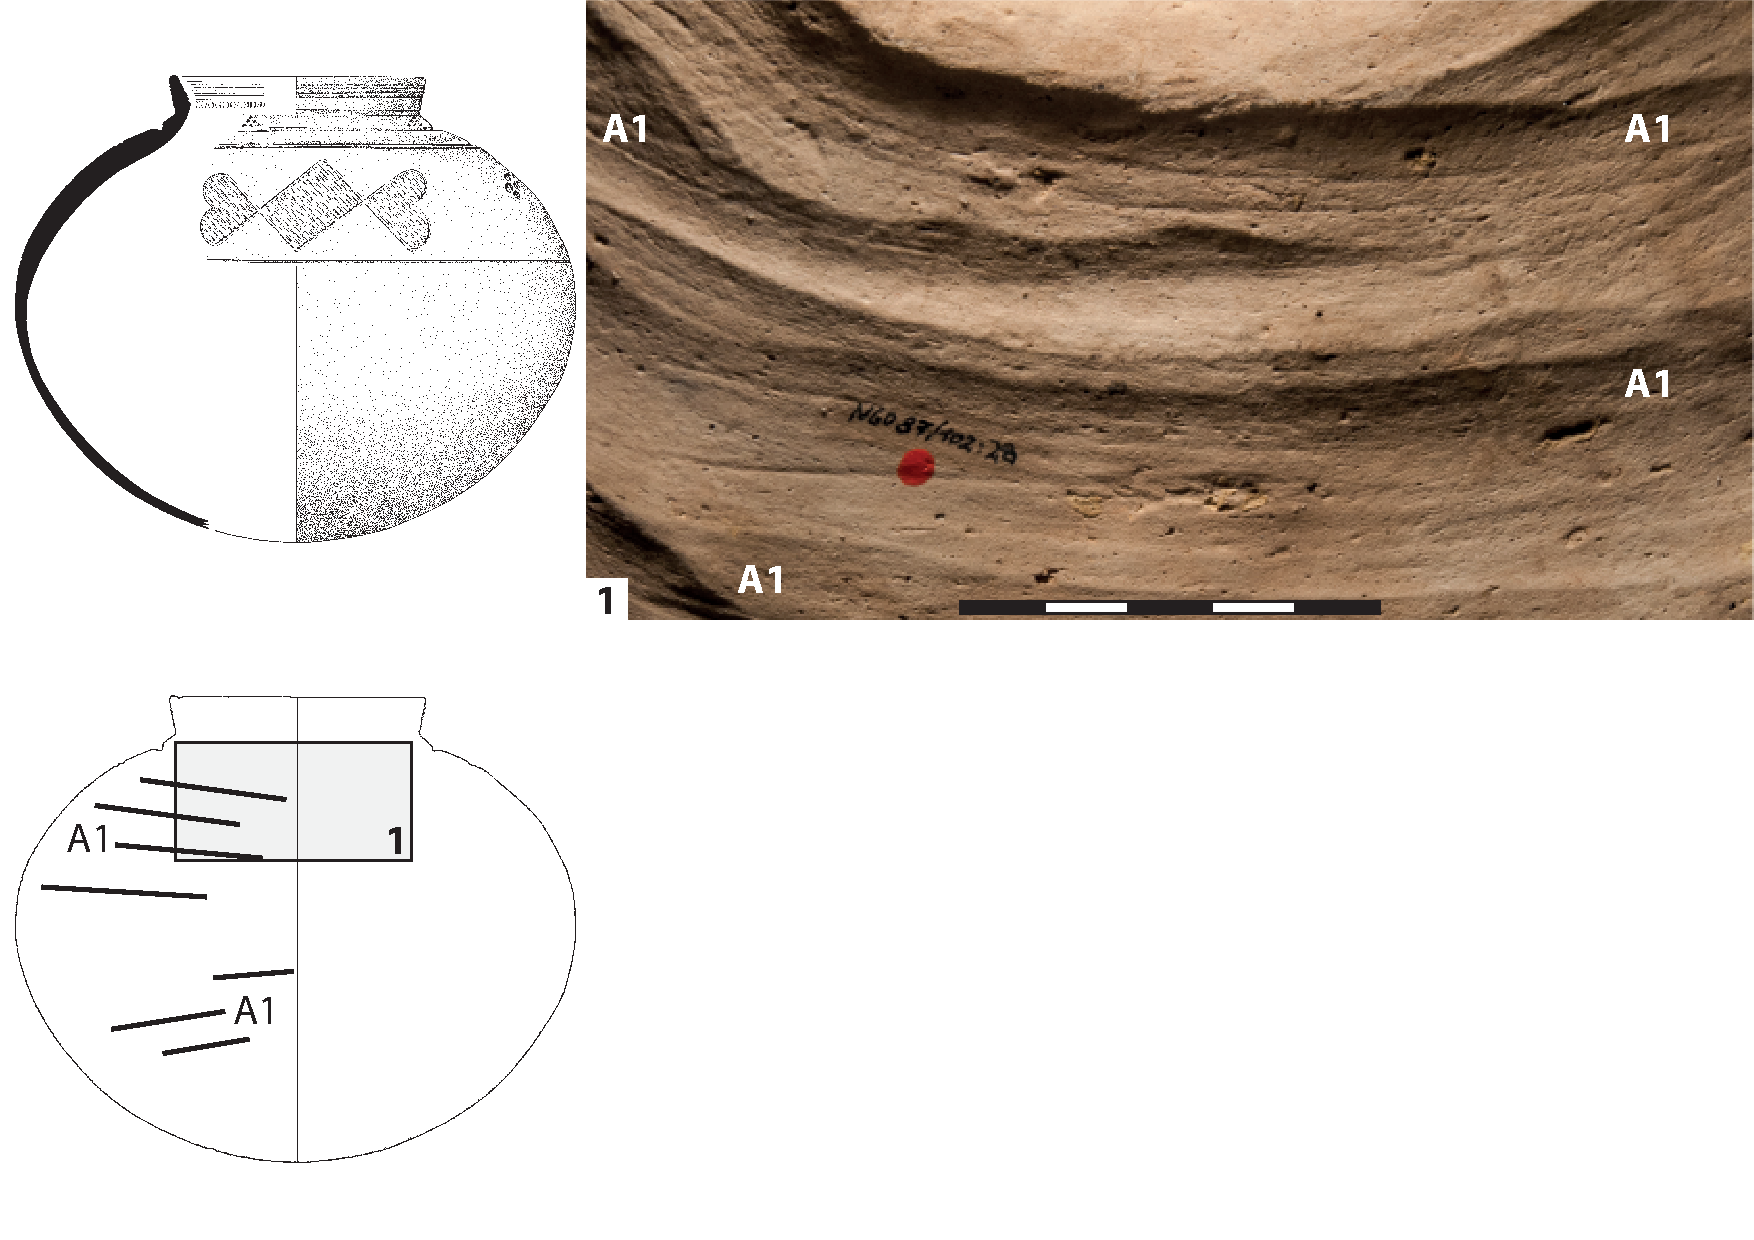
\includegraphics[width = \textwidth]{fig/Abb_Macrotraces/NGO87-102-28_29.pdf}
		\caption{Ngombe (Fpl.~252): Obj.~NGO~87/102:28--29 (Taf.~43.1).}
		\label{NGO87-102-28_29_Makrospuren}
	\end{subfigure}
	\caption{Makrospuren: Aufnahme und Details.}
\end{figure*}

Ein Gefäß der Batalimo-Maluba-Gruppe (Taf.~26.12), der ältesten entlang des \mbox{Ubangi} belegten keramischen Stilgruppe (Kap.~\ref{sec:BTM-Gr}), zeigt lediglich am Übergang von der Gefäßschulter zum Hals und dem größten Bauchdurchmesser einige wenige, leichte Glättspuren (A2a). Der Übergang zwischen Schulter und Hals ist innen durch eine scharfe Kante markiert, was andeutet, dass hier zwei separate Teile zusammengefügt wurden. Zwei GE der der Batalimo-Maluba-Gruppe stilistisch sehr nah stehenden Keramik, die vor allem entlang des mittleren \mbox{Ubangi} zu finden und als \mbox{Ngbanja}-Gruppe systematisiert ist (Kap.~\ref{sec:NGB-Gr}), wurden ebenfalls ausgewählt. Ein Gefäß aus dem eponymen Fundort \mbox{Ngbanja} weist innen im Bereich der Gefäßschulter und oberhalb der größten Gefäßweite einige eng sitzende leichte Glättspuren auf (Abb.~\ref{NGB85-101-130-01_Makrospuren}.1:~A2b), während der untere Teil gänzlich glatt ist. An einem zweiten, aus der gleichen Fundstelle stammenden Gefäß (Taf.~6.8) finden sich innen bis auf einige leichte Riefen im Bereich der größten Gefäßweite keinerlei Makrospuren. Die Keramik der \mbox{Ngbanja}-Gruppe zeichnet sich, wie auch die Batalimo-Maluba-Keramik, durch nur sehr wenige makroskopisch sichtbare Spuren aus, die Hinweise auf die Herstellung liefern können.

\begin{figure*}[p]
	\centering
	\begin{subfigure}{\textwidth}
		\centering
		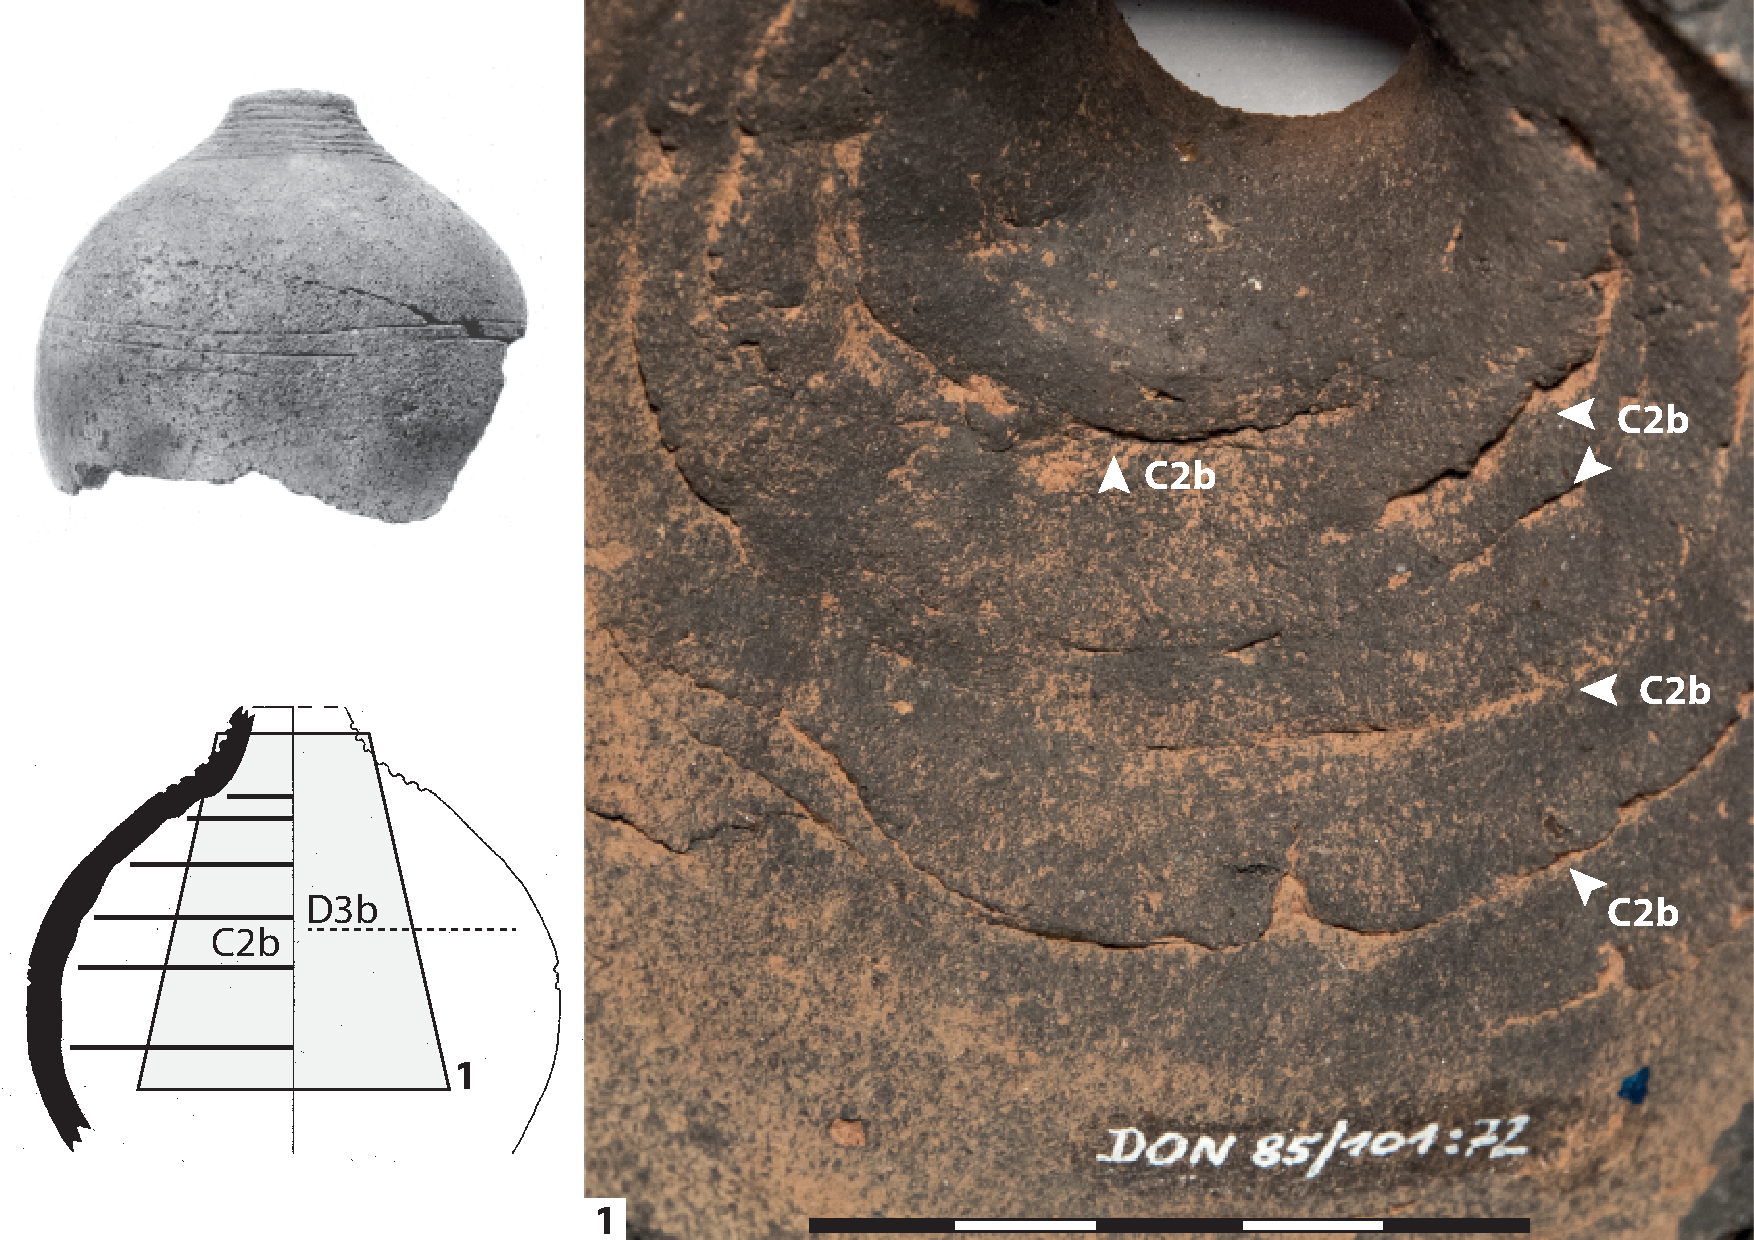
\includegraphics[width = \textwidth]{fig/Abb_Macrotraces/DON85-101-72.pdf}
		\caption{Dongo (Fpl.~202): Obj.~DON~85/101:72 (Taf.~7.14).\vspace{1em}}
		\label{DON85-101-71_Makrospuren}
	\end{subfigure}
	\begin{subfigure}{\textwidth}
		\centering
		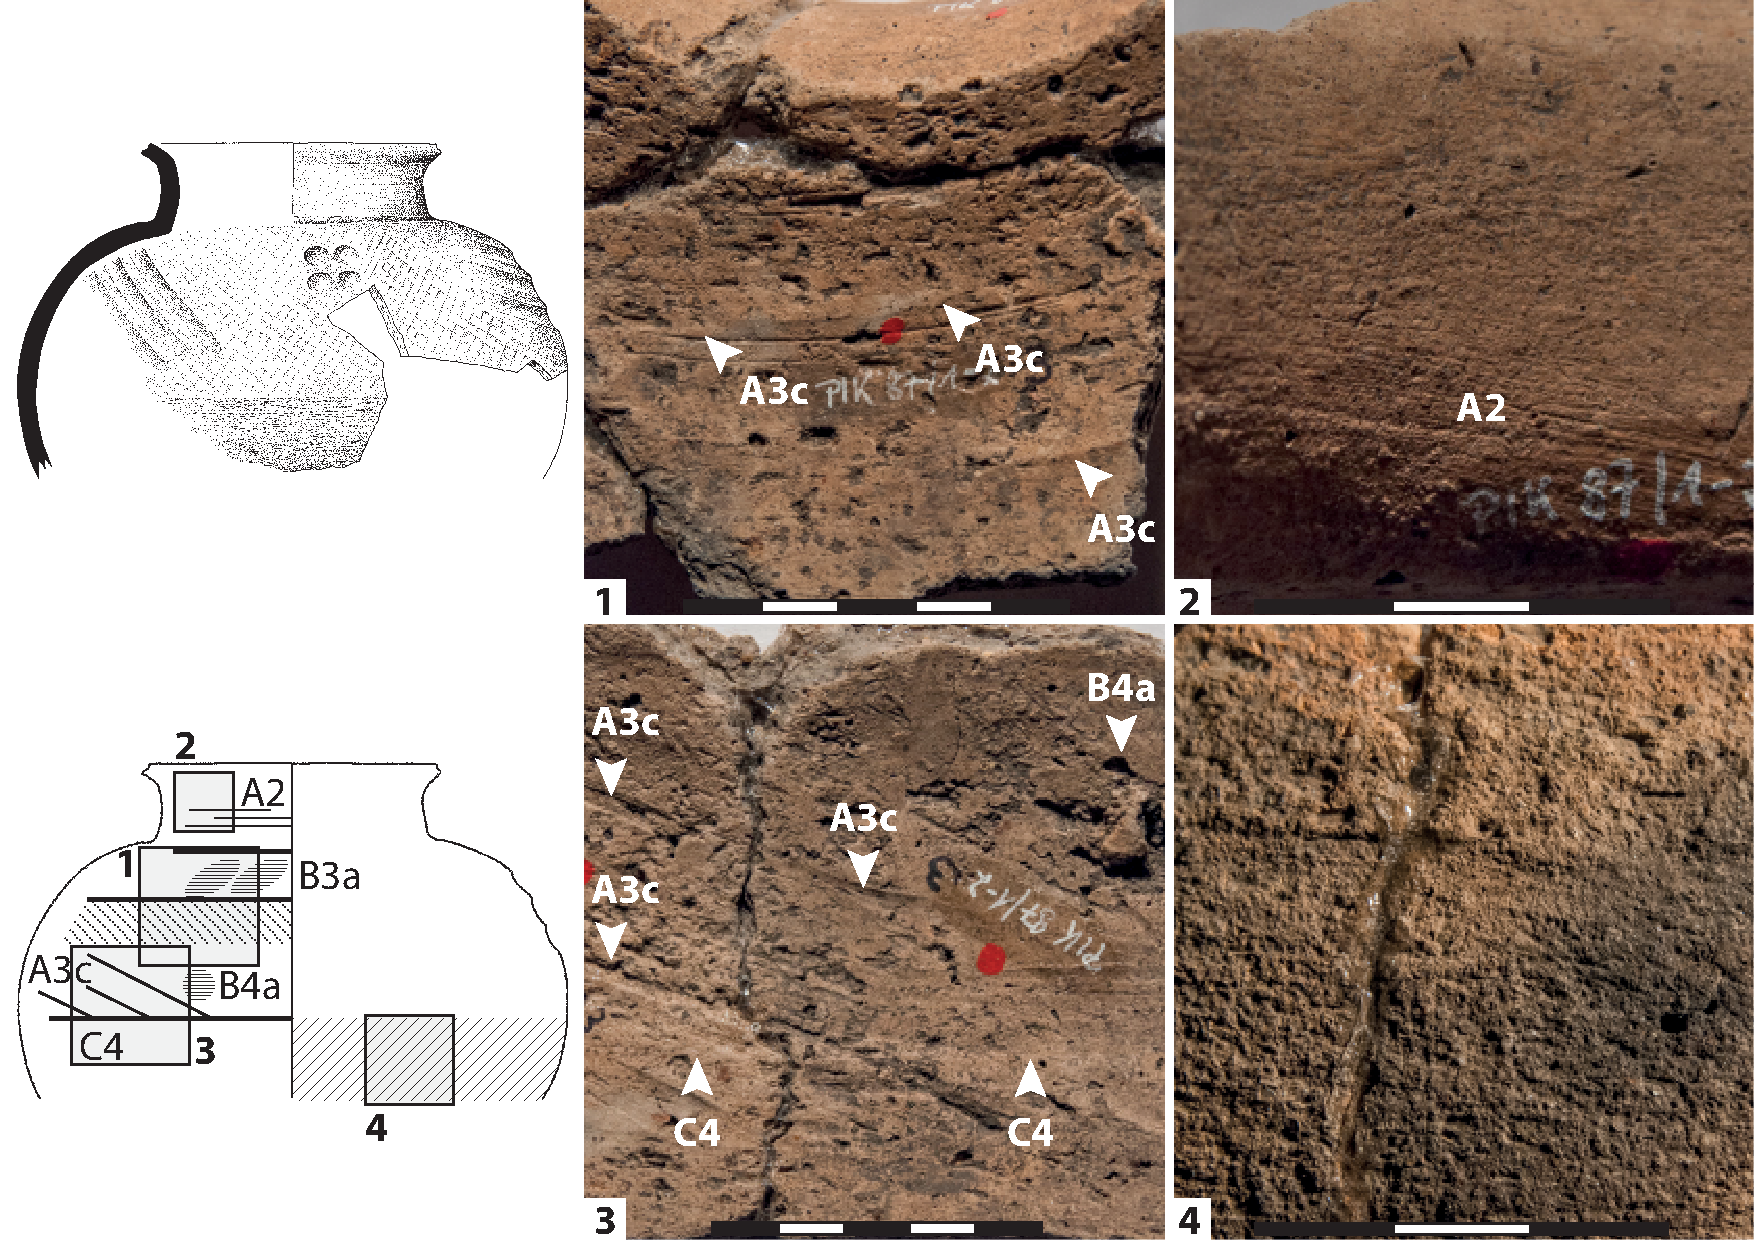
\includegraphics[width = \textwidth]{fig/Abb_Macrotraces/PIK87-1-2-3_1-3-7.pdf}
		\caption{Pikunda (Fpl.~255): Obj.~PIK~87/1-2:3 \& /1-3:7 (Taf.~47.24).}
		\label{PIK87-1-2-3_1-3-7_Makrospuren}
	\end{subfigure}
	\caption{Makrospuren: Aufnahme und Details.}
\end{figure*}

Die Keramik der Ngombe-Gruppe (Kap.~\ref{sec:NGO-Gr}) ist durch zwei formal durchaus unterschiedliche Gefäße repräsentiert. Beide stammen aus dem für die Beschreibung der Stilgruppe entscheidenden Befund in Ngombe am mittleren \mbox{Sangha} (Kat.-Nr.~11). Die Keramik dieser Stilgruppe weist formal starke Tendenzen zu Material aus dem Inneren Kongobecken auf, vor allem zur Longa-Gruppe \parencite[121--128]{Wotzka.1995}. Eine Knickwandschale zeigt im oberen Gefäßteil und nahe des Bodens feine horizontale Risse (D3a) sowie im Bereich des Bodens feine spiralige Glättspuren (Abb.~\ref{NGO87-102-27_Makrospuren}.1:~A2a). Der Boden des Gefäßes ist teilweise ausgebrochen und wurde eventuell erst zum Ende des Gefäßaufbaus geschlossen oder ausgearbeitet, wie die radialen Spuren im Bodenbereich andeuten. Das stark bauchige, zweite Gefäß weist innen Glättspuren eines konkaven Werkzeugs auf, die regelhaft etwa 20--25\,mm auseinander liegen (Abb.~\ref{NGO87-102-28_29_Makrospuren}.1:~A1). Zudem verlaufen die Bruchlinien des Gefäßes vor allem horizontal (D2a), was erfahrungsgemäß im Zusammenhang mit in Aufbautechnik hergestellter Keramik zu beobachten ist, bei der die Nahtbereiche zwischen den einzelnen Wülsten strukturelle Schwachstellen bilden.

Eine Flasche aus Dongo am \mbox{Ubangi} der gleichnamigen Stilgruppe (Kap.~\ref{sec:DON-Gr}) zeigt innen nicht verstrichene Wülste (Abb.~\ref{DON85-101-71_Makrospuren}.1:~C2b). Vor allem im Bereich unterhalb des Gefäßoberteils sind die Wülste nicht überarbeitet, während sie im Bereich des Unterteils größtenteils verstrichen sind. Dies deutet an, dass das Gefäß von unten nach oben aufgebaut wurde.

Stellvertretend für das Material der Mandombe-Gruppe (Kap.~\ref{sec:MDB-Gr}) wurden zwei Gefäße aus der in PIK~87/1 erfassten Grube A (siehe Kat.-Nr.~8) ausgewählt. Das erste Gefäß weist auf der Innenseite des fein geglätteten Halses leichte horizontale Glättspuren auf (Abb.~\ref{PIK87-1-2-3_1-3-7_Makrospuren}.2:~A2). Der innere Bereich unterhalb des Zylinderhalses ist rauer und nur grob überglättet. Unterhalb der Gefäßschulter befinden sich horizontale, flache Grate und fingerbreite leichte Eindrücke (B3a). Letzte sind möglicherweise das Resultat einer separat erfolgten Anbringung des Halses. Unterhalb der größten Gefäßweite, in etwa auf einer Höhe mit der außen aufgebrachten Schlickerrauung, befindet sich ein markanter, horizontal verlaufender, etwa 1\,mm breiter Absatz im Profil, unterhalb dessen die Wandung nach innen abrupt dicker wird (Abb.~\ref{PIK87-1-2-3_1-3-7_Makrospuren}.3:~C4). Oberhalb dieses Absatzes finden sich diagonal beziehungsweise spiralig nach oben laufende Glättrillen (A3c) und tiefe, bis etwa 1/3 in die Wandung ragende Eindrücke beziehungsweise Einbrüche der Gefäßwandung (Abb.~\ref{PIK87-1-2-3_1-3-7_Makrospuren}.3:~B4a). Das zweite, aus dem selben Befund stammende Gefäß weist innen ebenfalls horizontale, flache Erhöhungen beziehungsweise Grate und Senken auf (B3a; Taf.~47.22). Der Innenbereich des Gefäßes wurde lediglich grob überglättet, da noch viele durch ausgebrannte organische Partikel entstandene Porenräume sichtbar sind, während der Hals- und Randbereich innen -- wie auch die gesamte äußere Oberfläche -- fein geglättet und verstrichen ist. Innen, am für die Gefäße der Mandombe-Gruppe charakteristischen Zylinderhals, finden sich kurze, vertikale Risse (D3a) und Rillen (A2a). Der Übergang zwischen Gefäßbauch und -hals wird innen durch einen deutlichen Umbruch markiert. Es kann angenommen werden, dass der Halsbereich als separates Element aufgesetzt wurde. Beiden Stücken ist gemein, dass die Innenseite zwar grob geglättet wurde, wie die sichtbaren Glättspuren belegen (Abb.~\ref{PIK87-1-2-3_1-3-7_Makrospuren}.1, 3), die Oberfläche an allen sichtbaren Partien aber noch einmal besonders bearbeitet und geglättet wurde, wie die sehr feinen, eng sitzende Glättspuren im Halsbereich der Gefäße anzeigen (siehe Abb.~\ref{PIK87-1-2-3_1-3-7_Makrospuren}.2). Diese könnten auf ein Überglätten der betreffenden Stellen mit Stoff oder Leder hindeuten; möglicherweise wurden die Bereiche hierzu auch noch einmal leicht angefeuchtet. Spuren der im Scherben vorhandenen, nunmehr ausgebrannten Organik lassen sich im nicht entsprechend behandelten Innenbereiche der Gefäße erkennen. Eine systematische Modifikation bildet auch der Auftrag eines groben Schlickers auf der Gefäßunterseite (siehe Abb.~\ref{PIK87-1-2-3_1-3-7_Makrospuren}.4).

Zwei Randstücke der Konda-Gruppe (Kap.~\ref{sec:KON-Gr}), beide aus dem namensgebenden Fundplatz Konda (Fpl.~268) am oberen \mbox{Sangha}, weisen innen im Schulterbereich horizontalen Vertiefungen auf, die als Überreste nicht vollständig verstrichener Zwischenräume zwischen Wülsten angesprochen werden können (C2b). Für beide Stücke kann zumindest für den oberen Teil des Gefäßes eine Wulstaufbautechnik postuliert werden. Da keine Bodenstücke der Konda-Gruppe bekannt sind, muss die Herstellungstechnik des Unterteils der Konda-Gefäße als unbekannt gelten.

Die rezente Keramik am Likwala-aux-Herbes, die unter der Bezeichnung Epena-Gruppe (Kap.~\ref{sec:EPE-Gr}) zusammengefasst wurde, ist durch zwei Stücke vertreten. Ein Gefäß aus Jeke zeichnet sich innen durch deutliche Makrospuren aus. Im Rand- wie im gesamten inneren Bauchbereich befinden sich diagonal spiralig aufsteigende Grate (Abb.~\ref{JEK87-103-57_Makrospuren}.1:~A1). Sie weisen einen Abstand von etwa 20--30\,mm zueinander auf. Im unteren Gefäßteil beziehungsweise im Bereich des Bodenansatzes sind diese Grate von überkreuzten, ebenfalls diagonal aufsteigenden Riefen überlagert (A1). Im Schulterbereich finden sich tiefe Werkzeugspuren (Abb.~\ref{JEK87-103-57_Makrospuren}.2:~B4a), die auf das Zusammenfügen eines separat gefertigten Hals- und Randbereiches sowie des Gefäßkörpers hindeuten. Die Außenseite des Gefäßunterteils ist vertikal ziehharmonikaartig verformt (Abb.~\ref{JEK87-103-57_Makrospuren}.3:~C1). Dies kann als Hinweis gedeutet werden, dass der Boden und die Gefäßunterseite erst gegen Ende geschlossen beziehungsweise ausgeformt wurden. Eine Flasche aus Itanga zeichnet sich innen durch spiral aufsteigende Grate aus (Abb.~\ref{ITN87-103_Makrospuren}.1:~A1). Diese weisen einen durchgehenden Abstand von etwa 25\,mm auf, und die konkaven Vertiefungen lassen auf die Glättung der Innenseite durch eine Muschel oder ein ähnliches Werkzeug schließen. Der Halsbereich wurde in einem getrennten Arbeitsschritt ausgeformt, weist innen vertikale Riefen (Abb.~\ref{ITN87-103_Makrospuren}.1:~A3b) auf, die eventuell auf eine Komprimierung des Materials hindeuten, und wurde dann mit dem Gefäßkörper verbunden. Die unter der Gefäßschulter sichtbaren tiefen Eindrücke (Abb.~\ref{ITN87-103_Makrospuren}.1:~B4a) deuten auf die Nutzung eines Werkzeugs hin, um die Verbindung herzustellen. Der Boden des Gefäßes ist nicht erhalten. Die äußere Wandung ist ebenfalls, wie schon bei dem Gefäß aus Jeke, ziehharmonikaartig verformt (Abb.~\ref{ITN87-103_Makrospuren}.2:~C1), was auf eine Komprimierung von Material hindeutet.

Die Epena-Keramik lässt sich deutlich aus dem formalen Spektrum der Ebambe-Keramik ableiten (Kap.~\ref{sec:EBA-Gr}). Um den starken Bezug der beiden Stilgruppen näher zu beleuchten, wurden zwei in Munda am oberen \mbox{Likwala}-\mbox{aux}-\mbox{Herbes} (Fpl.~304) und eine aus Pikunda am mittleren \mbox{Sangha} (Fpl.~255) stammende GE ausgewählt.\footnote{Die Herstellung einer entsprechenden Flasche mit langem Kegelhals, die formal der Ebambe-Gruppe zugerechnet werden kann, wurde 1987 in Boleko am unteren \mbox{Likwala}-\mbox{aux}-\mbox{Herbes} (Fpl.~285) beobachtet. Siehe Anm.~\ref{ftn:EthnoToepfereiInVorb}.} Eines der beiden aus Munda stammenden Gefäße weist innen markante spiralig nach oben laufende, feine Riefen beziehungsweise Grate auf (Abb.~\ref{MUN87-1-0-2-1-3_Makrospuren}.2:~A1). Unterhalb des Schulterbereiches befinden sich weitere spiralig nach oben laufende Grate (A1). Der Übergang vom Gefäßbauch zum Halsbereich ist ebenfalls durch einen deutlichen Grat markiert. Im Hals- und Randbereich des Gefäßes sind feine Glättspuren zu beobachten (Abb.~\ref{MUN87-1-0-2-1-3_Makrospuren}.1:~A2a). Im Zentrum des leicht einziehenden Bodens befindet sich eine Verdickung, die von sternförmig verlaufenden Rissen durchzogen ist (Abb.~\ref{MUN87-1-0-2-1-3_Makrospuren}.3:~C3a, D3c). Dieses Merkmal kann als Hinweis darauf gedeutet werden, dass der Boden des Gefäßes erst zum Ende des Herstellungsprozesses geschlossen wurde, wobei in geringem Maße überschüssiges Material anfiel. Eine ebenfalls aus Munda stammende Flasche weist innen, vor allem im Schulterbereich, die gleichen, diagonal aufsteigenden flachen Grate auf (Abb.~\ref{MUN87-1-0-2-6-2_Makrospuren}.1:~A1). Der flache Boden zeichnet sich durch eine mit feinen Rissen durchzogene Verdickung aus (Abb.~\ref{MUN87-1-0-2-6-2_Makrospuren}.2:~C3a, D3c). Dies kann darauf hindeuten, dass der Boden dieses Gefäßes erst zum Ende des Herstellungsprozesses geschlossen wurde. Der tiefe, vertikal verlaufende Eintiefungen aufweisende Hals scheint in einem gesonderten Arbeitsprozess ausgeformt worden zu sein (Abb.~\ref{MUN87-1-0-2-6-2_Makrospuren}.1:~A3b). Die vertikalen, ziehharmonikaartigen Eintiefungen können das Resultat einer Verengung des Materials und einer damit einhergehenden Komprimierung sein. Das aus Pikunda am \mbox{Sangha} stammende und der Ebambe-Gruppe (Taf.~49.16) zuzurechnende Gefäßfragment zeigt im Schulterbereich feine Glättspuren (A2a) und kleine Eintiefungen (B3b). Am Gefäßbauch befinden sich diagonale bis vertikale fingerbreite Eindrücke (B3a). Die Außenseite ist im unteren Bereich des Gefäßbauches kaum geglättet und leicht rau.

\begin{figure*}[p]
	\centering
	\begin{subfigure}{\textwidth}
		\centering
		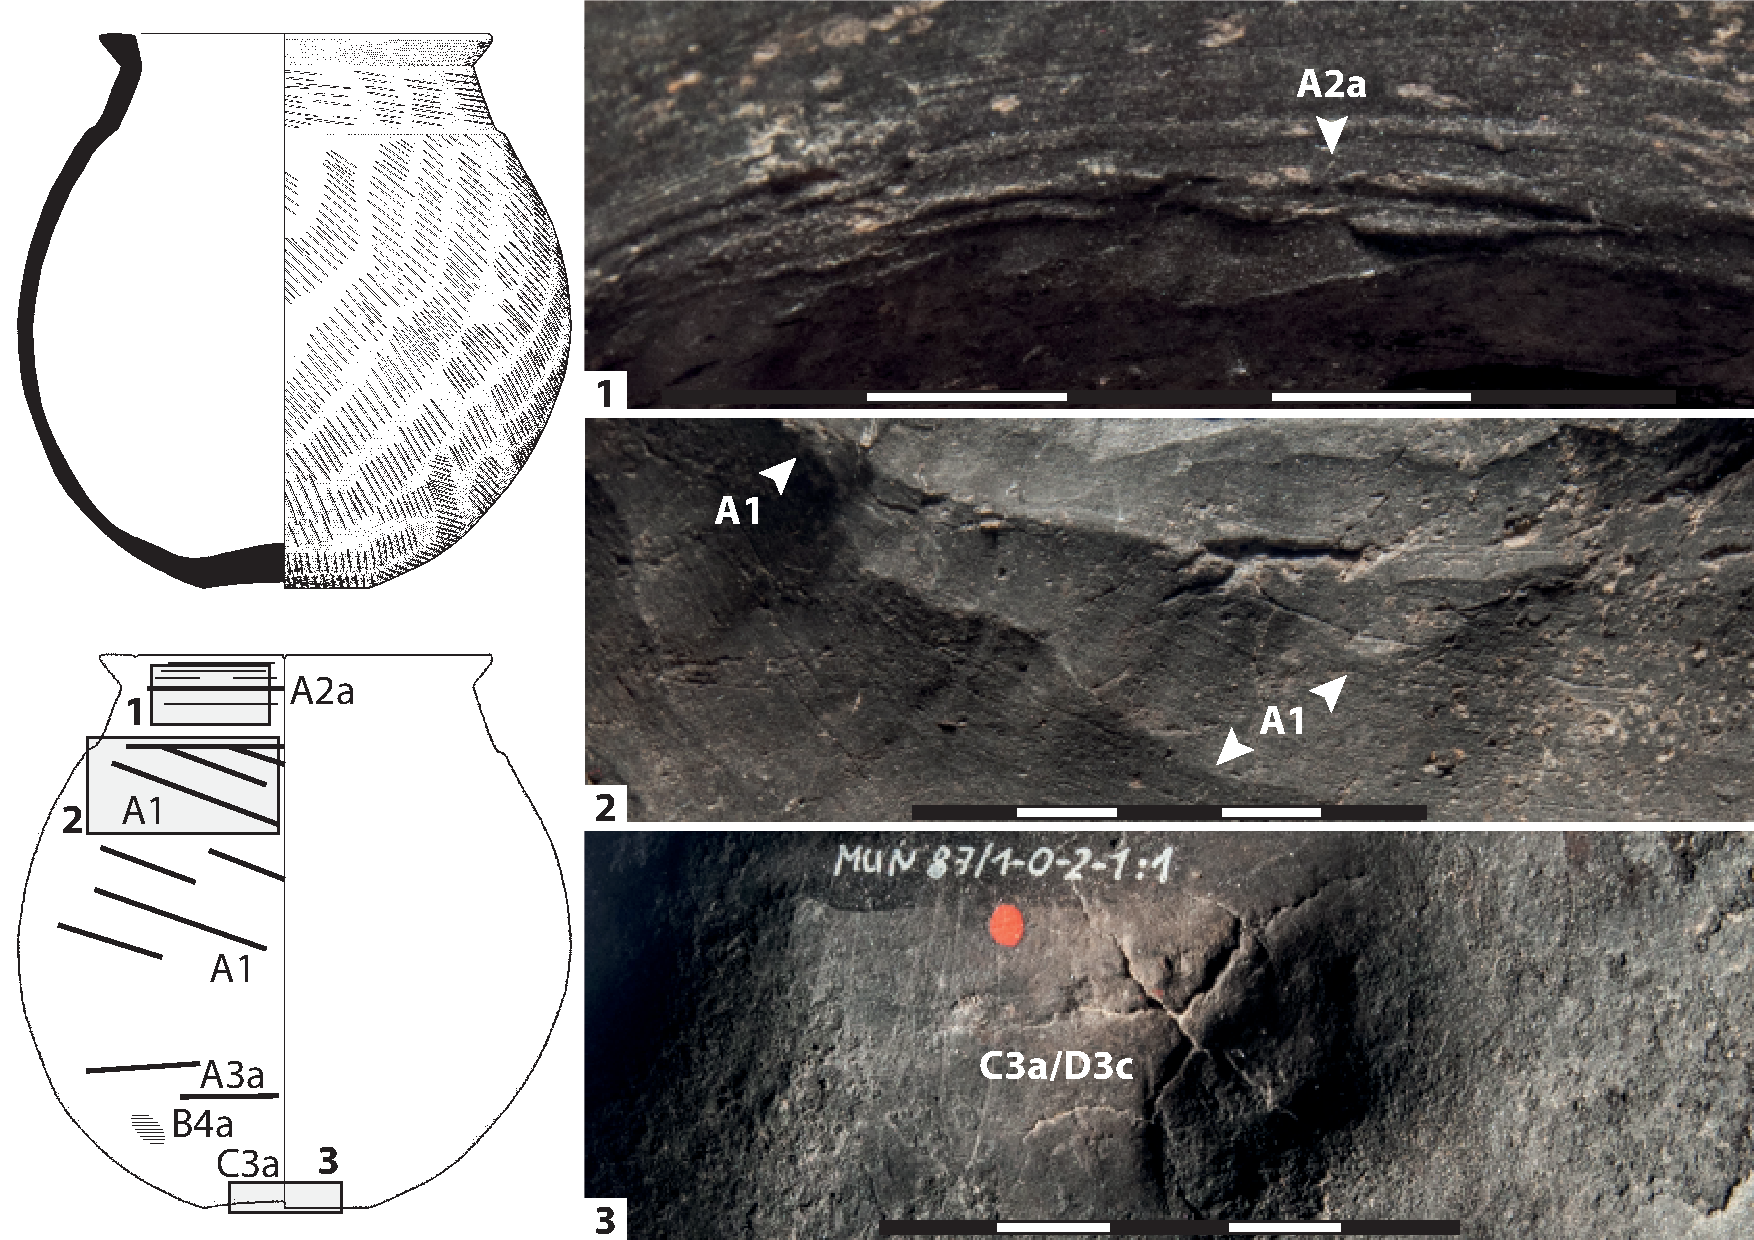
\includegraphics[width = \textwidth]{fig/Abb_Macrotraces/MUN87-1-0-2-1-1.pdf}
		\caption{Munda (Fpl.~304): Obj.~MUN~87/1-0-2-1:3 (Taf.~89.4).\vspace{1em}}
		\label{MUN87-1-0-2-1-3_Makrospuren}
	\end{subfigure}
	\begin{subfigure}{\textwidth}
		\centering
		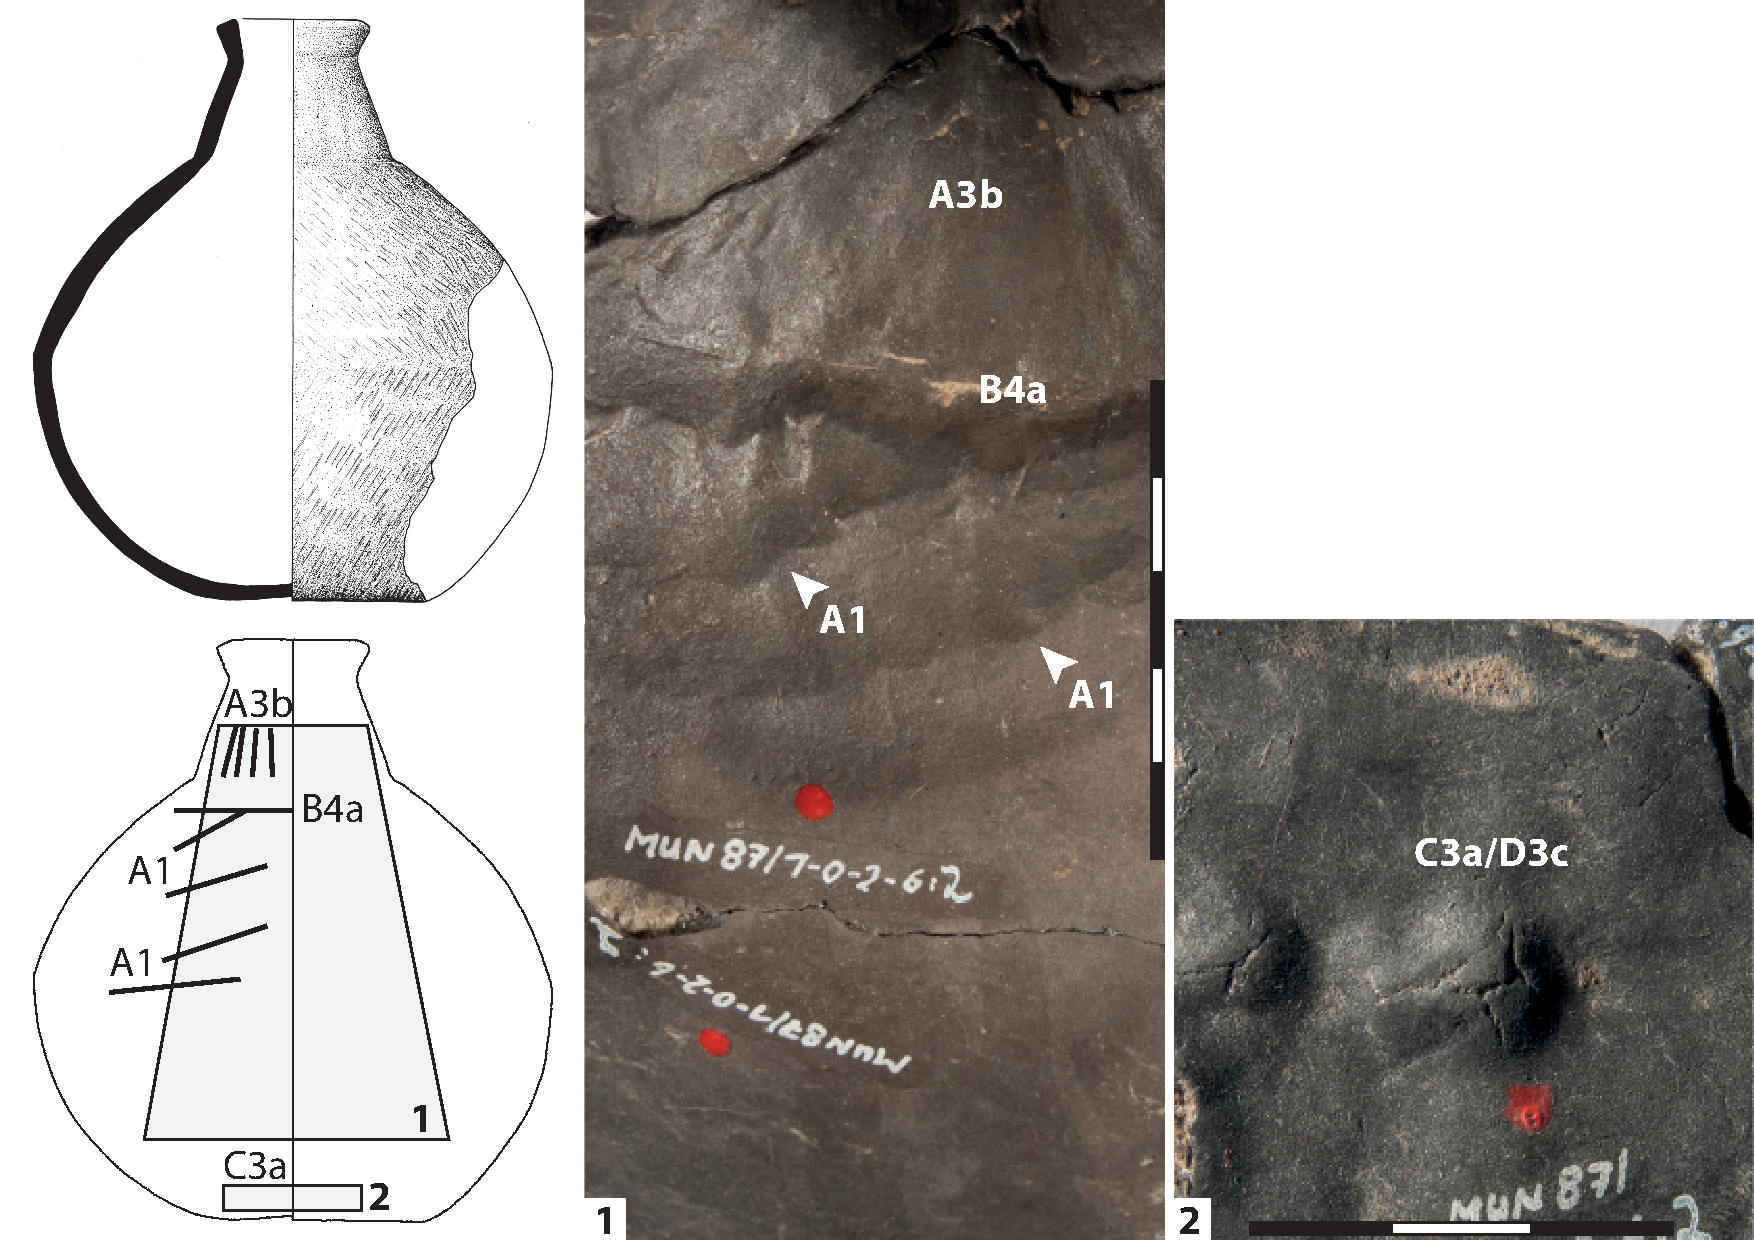
\includegraphics[width = \textwidth]{fig/Abb_Macrotraces/MUN87-1-0-2-6-2.pdf}
		\caption{Munda (Fpl.~304): Obj.~MUN~87/1-0-2-6:2 (Taf.~90.1).}
		\label{MUN87-1-0-2-6-2_Makrospuren}
	\end{subfigure}
	\caption{Makrospuren: Aufnahme und Details.}
\end{figure*}

\begin{figure*}[p]
	\centering
	\begin{subfigure}{\textwidth}
		\centering
		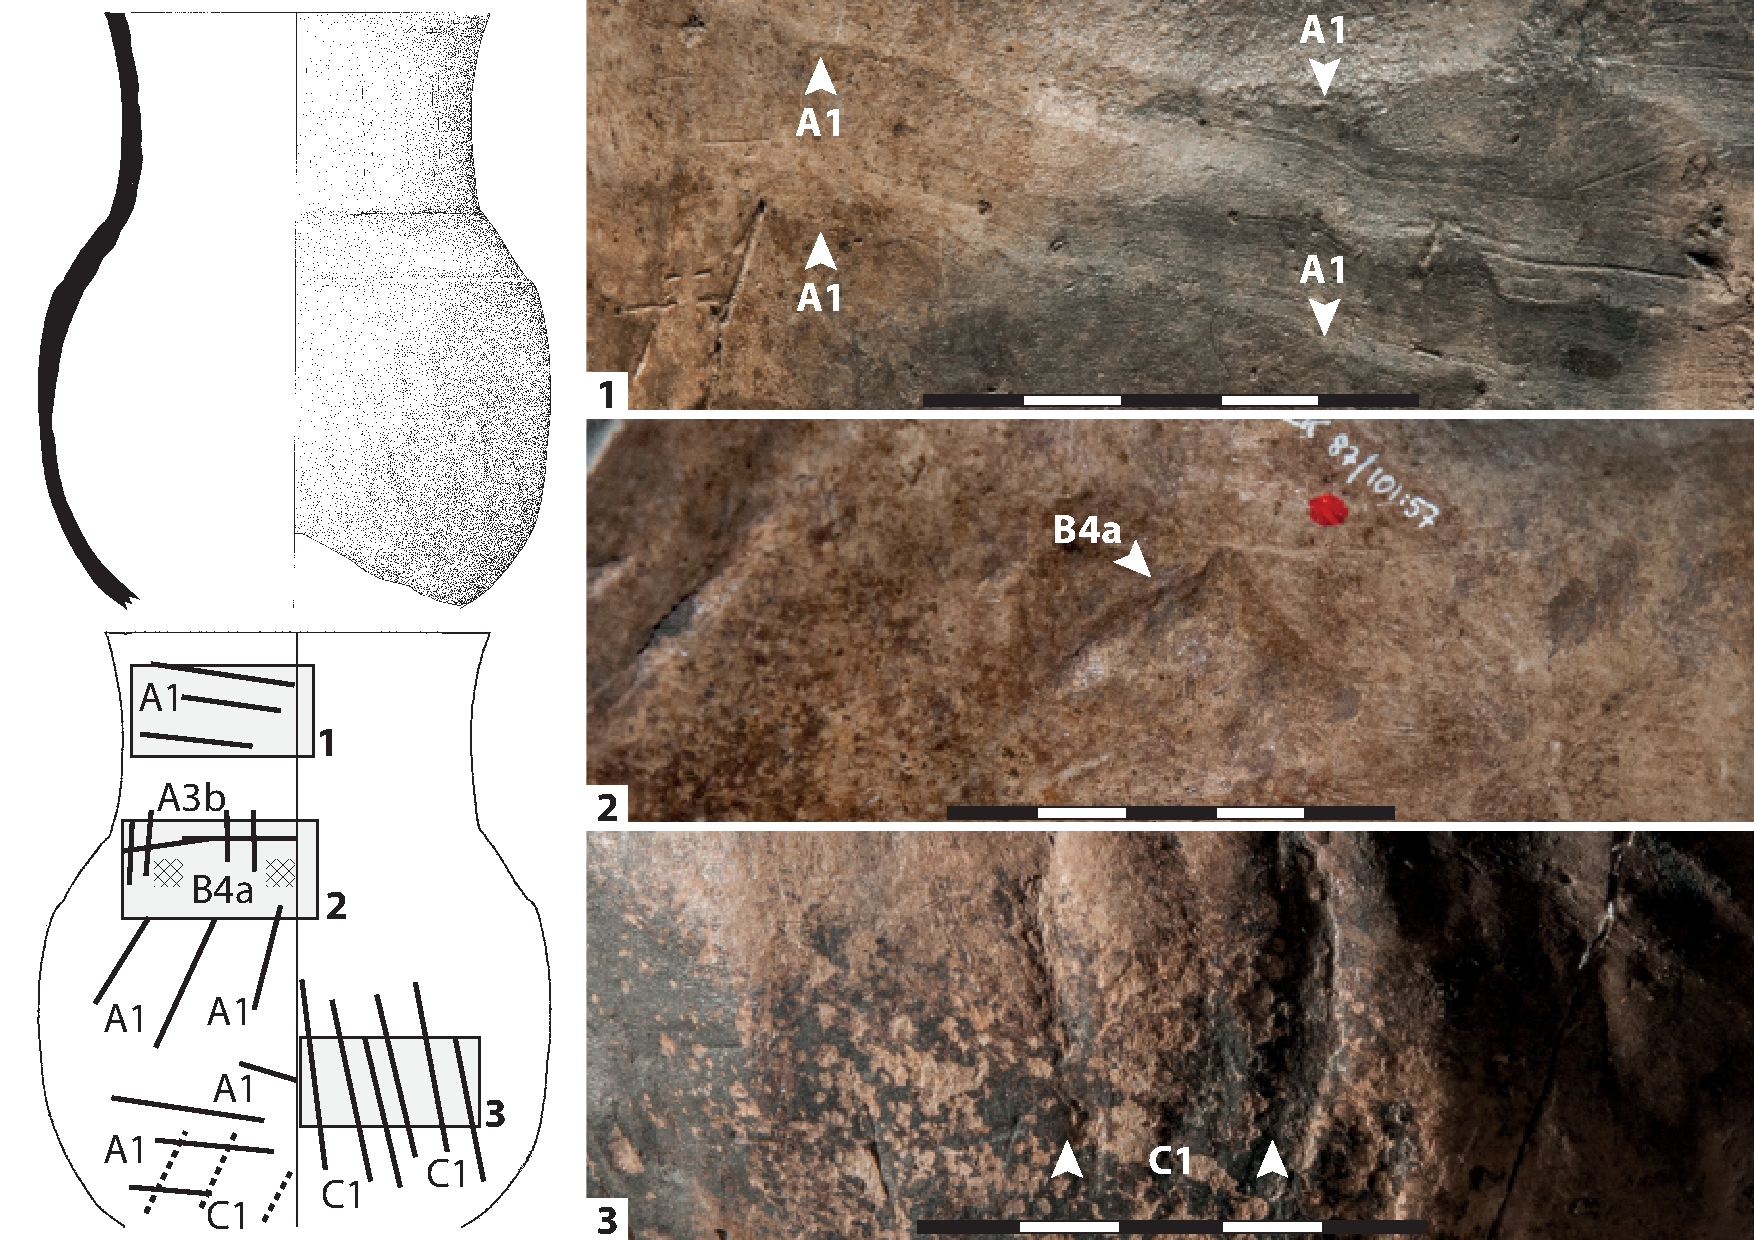
\includegraphics[width = \textwidth]{fig/Abb_Macrotraces/JEK87-101-57.pdf}
		\caption{Jeke (Fpl.~303): Obj.~JEK~87/101:57 (Taf.~88.1).\vspace{1em}}
		\label{JEK87-103-57_Makrospuren}
	\end{subfigure}
	\begin{subfigure}{\textwidth}
		\centering
		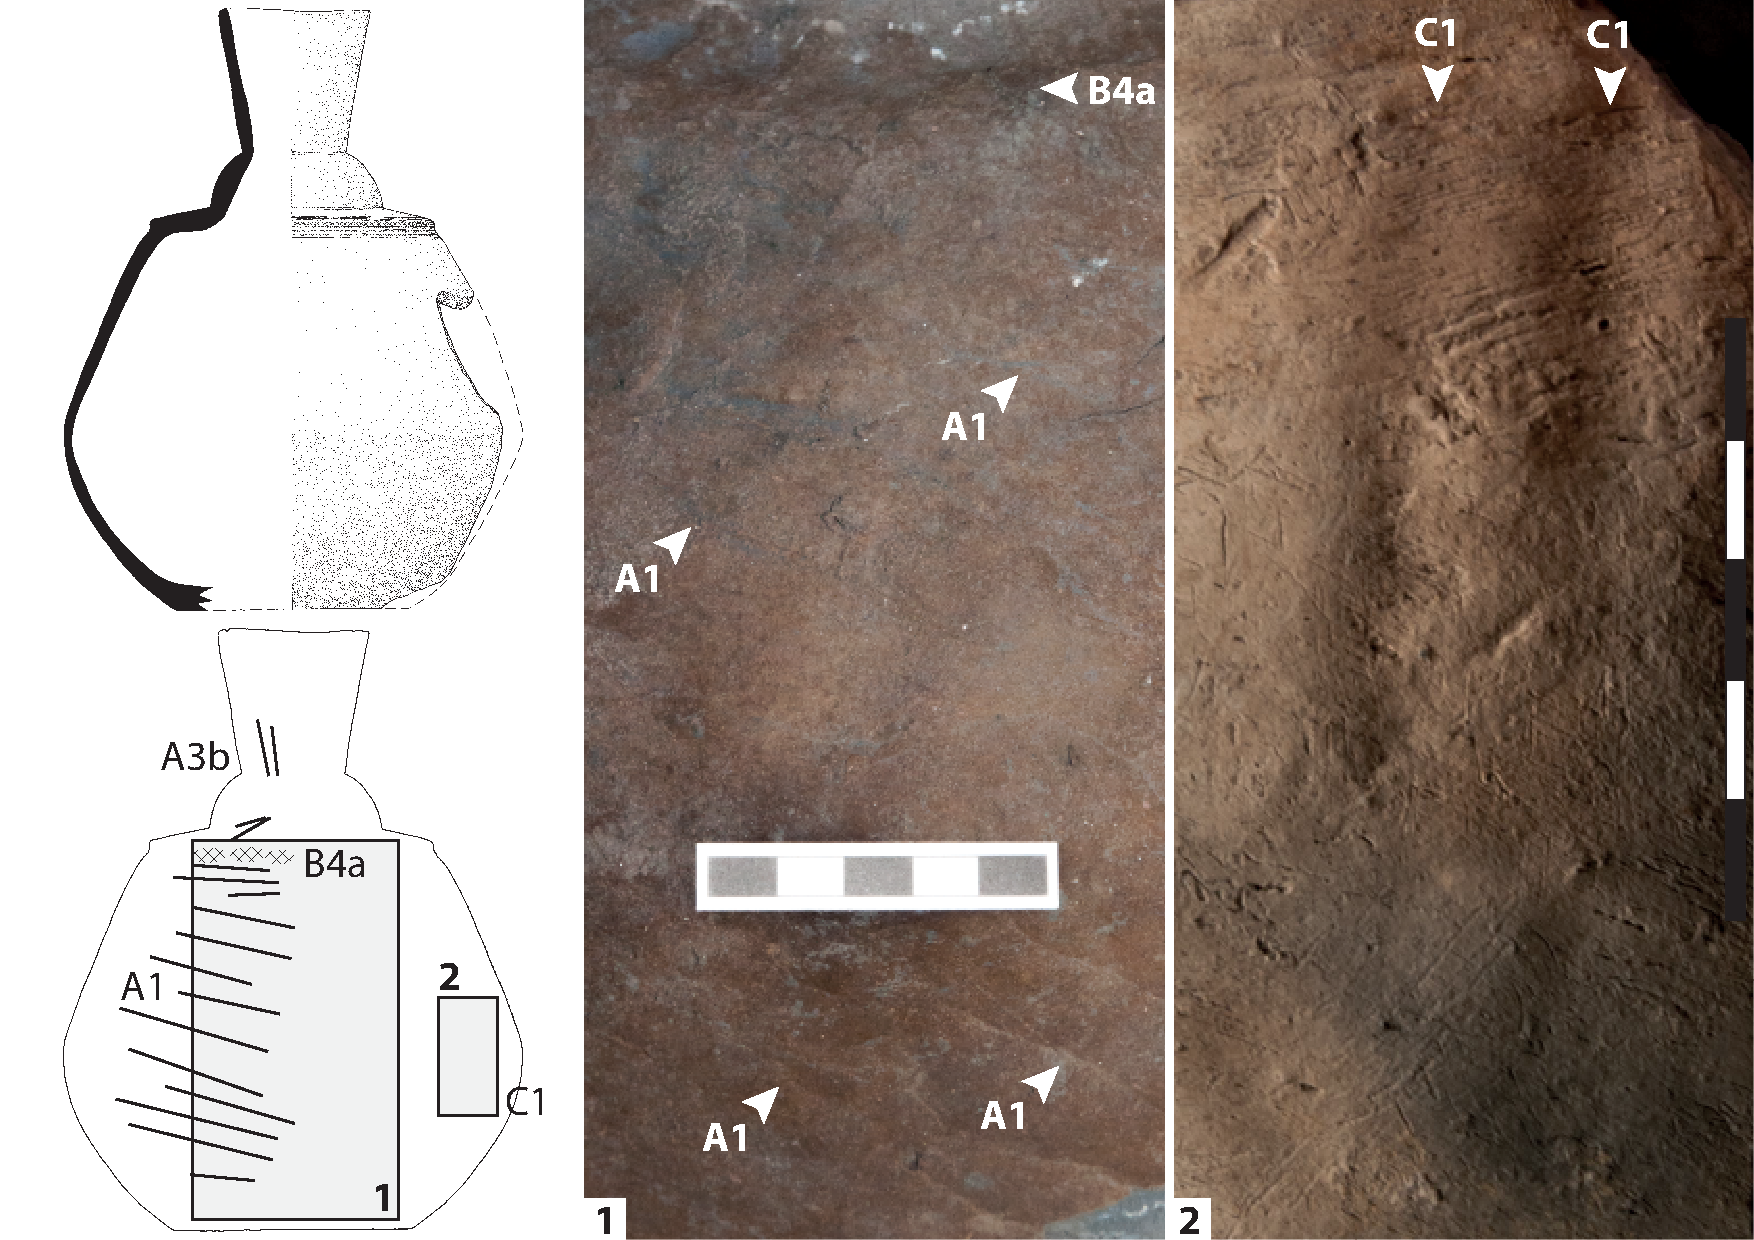
\includegraphics[width = \textwidth]{fig/Abb_Macrotraces/ITN87-103.pdf}
		\caption{Itanga (Fpl.~305): Obj.~ITN~87/103 (Taf.~97.4).}
		\label{ITN87-103_Makrospuren}
	\end{subfigure}
	\caption{Makrospuren: Aufnahme und Details.}
\end{figure*}

\begin{figure*}[p]
	\centering
	\begin{subfigure}{\textwidth}
		\centering
		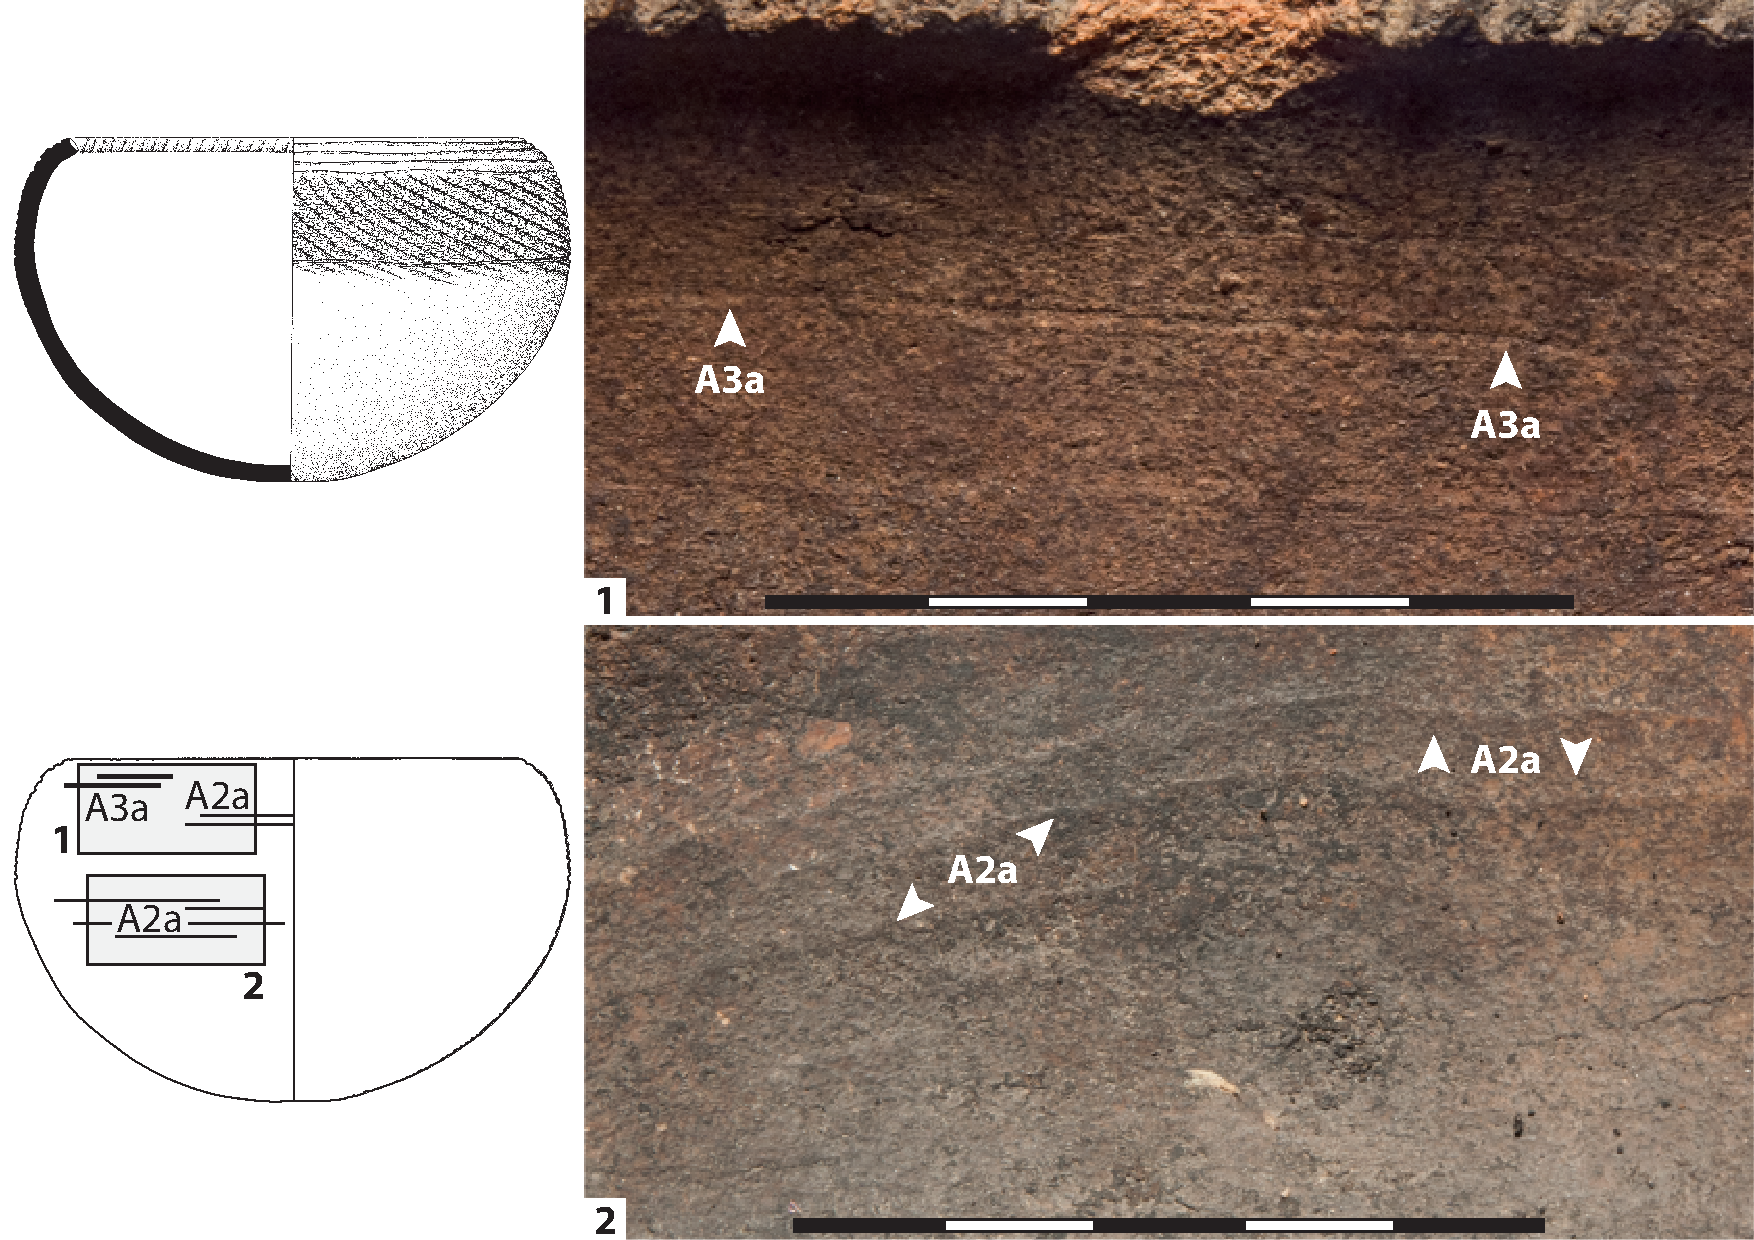
\includegraphics[width = \textwidth]{fig/Abb_Macrotraces/MBN85-501-1.pdf}
		\caption{Mbati-Ngombe (Fpl.~204): Obj.~MBN~85/501:1 (Taf.~11.1).\vspace{1em}}
		\label{MBN85-501-1_Makrospuren}
	\end{subfigure}
	\begin{subfigure}{\textwidth}
		\centering
		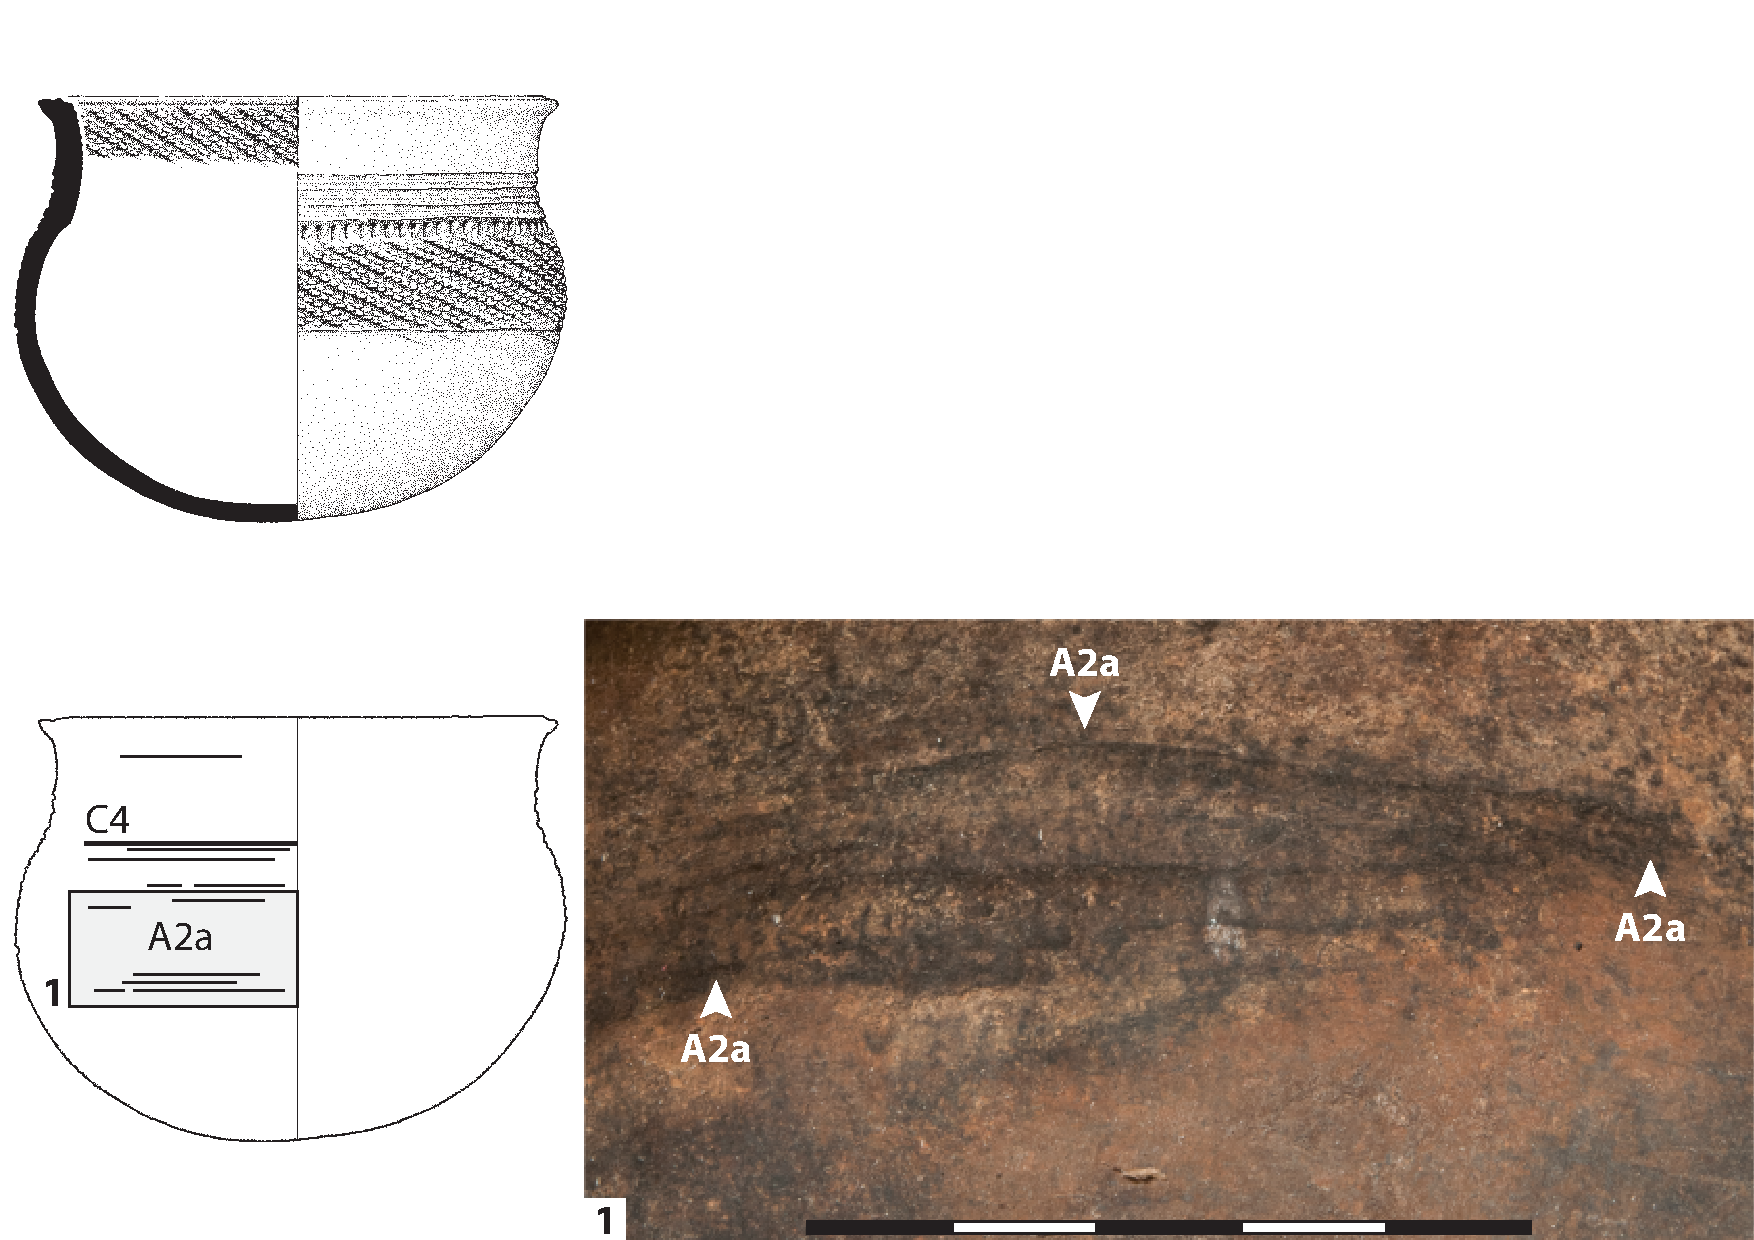
\includegraphics[width = \textwidth]{fig/Abb_Macrotraces/MBN85-501-2.pdf}
		\caption{Mbati-Ngombe (Fpl.~204): Obj.~MBN~85/501:2 (Taf.~11.2).}
		\label{MBN85-501-2_Makrospuren}
	\end{subfigure}
	\caption{Makrospuren: Aufnahme und Details.}
\end{figure*}

Die rezente Keramik entlang des mittleren \mbox{Ubangi}, repräsentiert durch die Mbati-Ngombe-Gruppe (Kap.~\ref{sec:MBN-Gr}), ist durch zwei GE aus dem eponymen Fundort (Fpl.~204) in der Untersuchung vertreten. Das Unterteil des ersten Gefäßes zeigt keine Makrospuren und der runde Boden weist nur leichte Unregelmäßigkeiten auf, während sich im oberen Bereich leichte, horizontale Glättspuren beobachten lassen (Abb.~\ref{MBN85-501-1_Makrospuren}.2:~A2a). Unterhalb des Randes finden sich zudem kurze, tiefere Glättriefen (Abb.~\ref{MBN85-501-1_Makrospuren}.1:~A3a). Das zweite Gefäß zeichnet sich innen auch durch feine, horizontale Glättspuren aus (Abb.~\ref{MBN85-501-2_Makrospuren}.1:~A2a). Im Bereich des Übergangs vom Bauch- zum Halsbereich zeigt sich ein horizontal verlaufender Grat (C4). Der Innenbereich des Gefäßbodens ist auffällig glatt und der runde Boden regelmäßig geformt.\columnbreak

\begin{figure*}[p]
	\centering
	\begin{subfigure}{\textwidth}
		\centering
		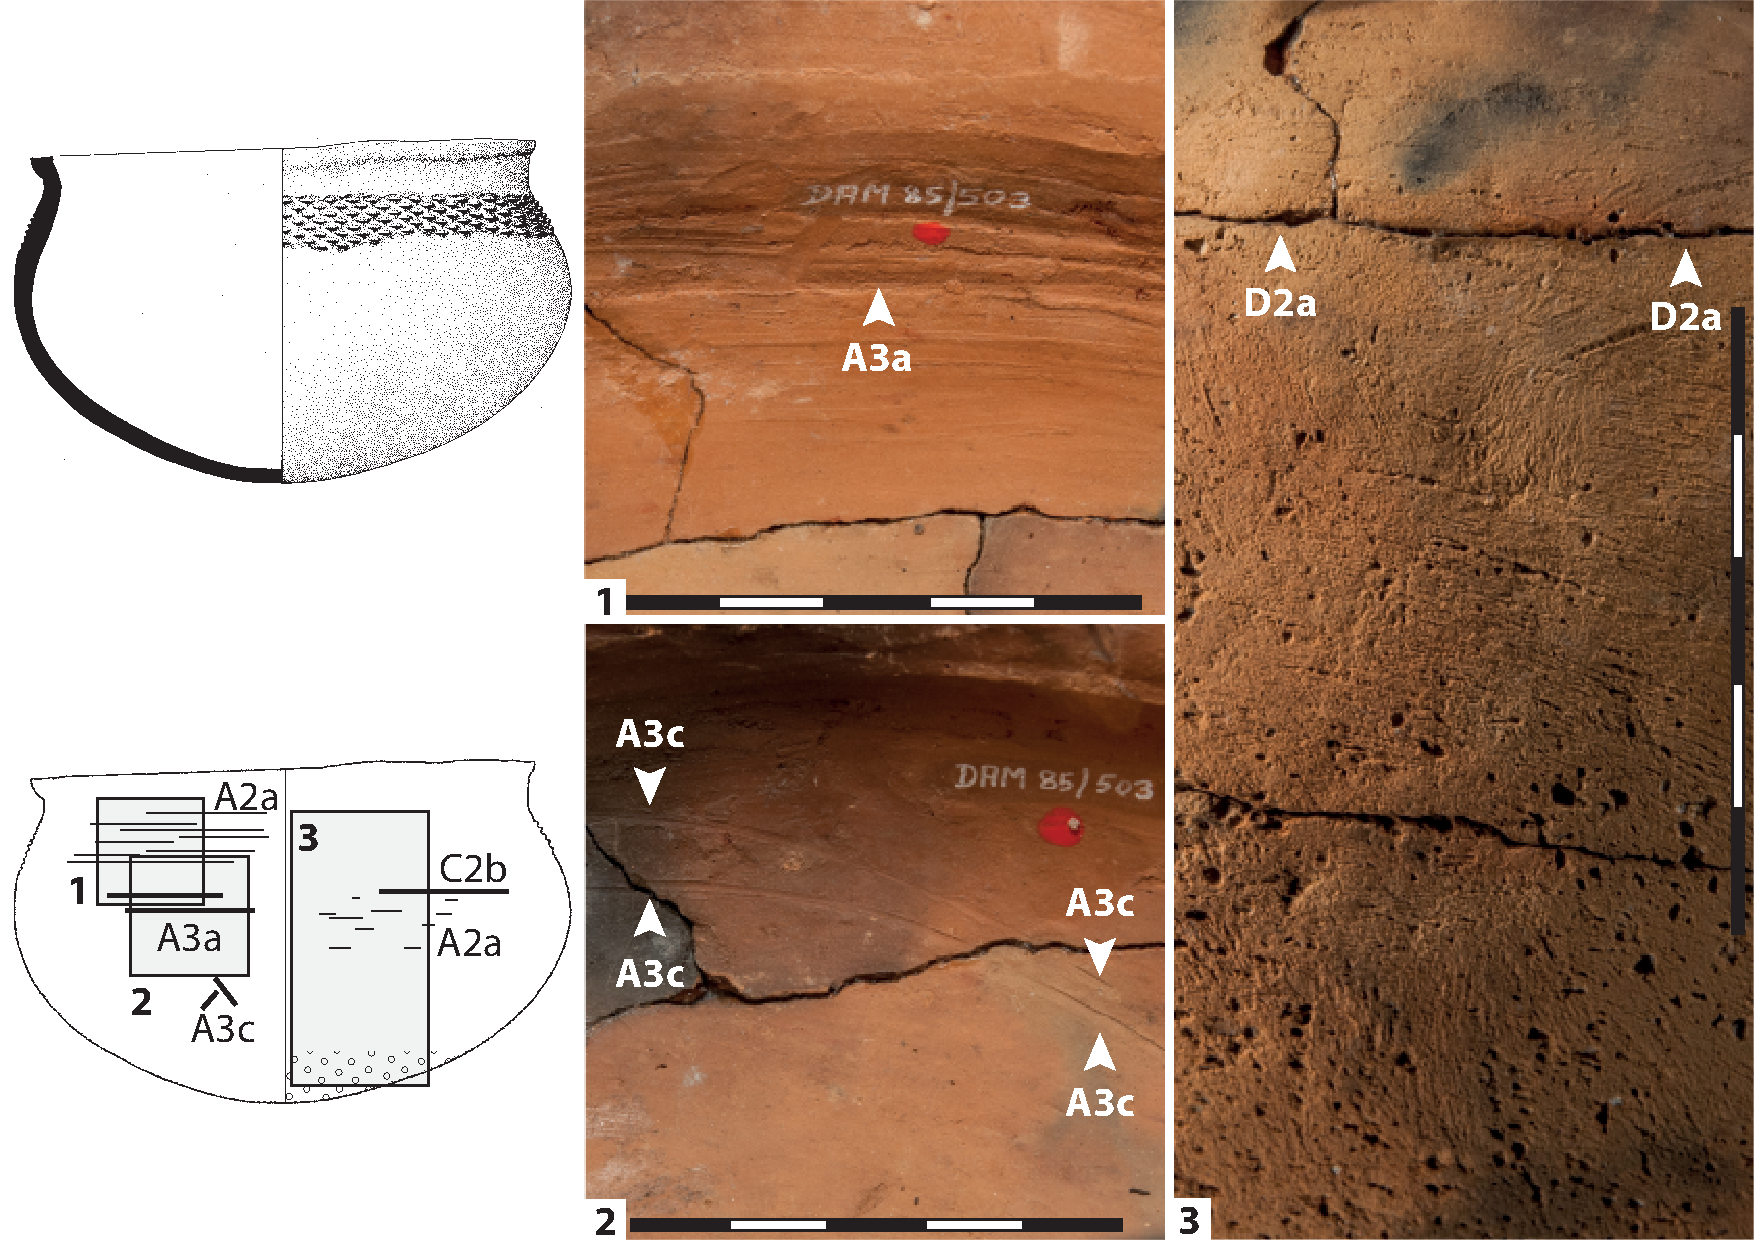
\includegraphics[width = \textwidth]{fig/Abb_Macrotraces/DAM85-503-a.pdf}
		\caption{Dama (Fpl.~222): Obj.~DAM~85/503:1 (Taf.~23.2).\vspace{1em}}
		\label{DAM85-503-1_Makrospuren}
	\end{subfigure}
	\begin{subfigure}{\textwidth}
		\centering
		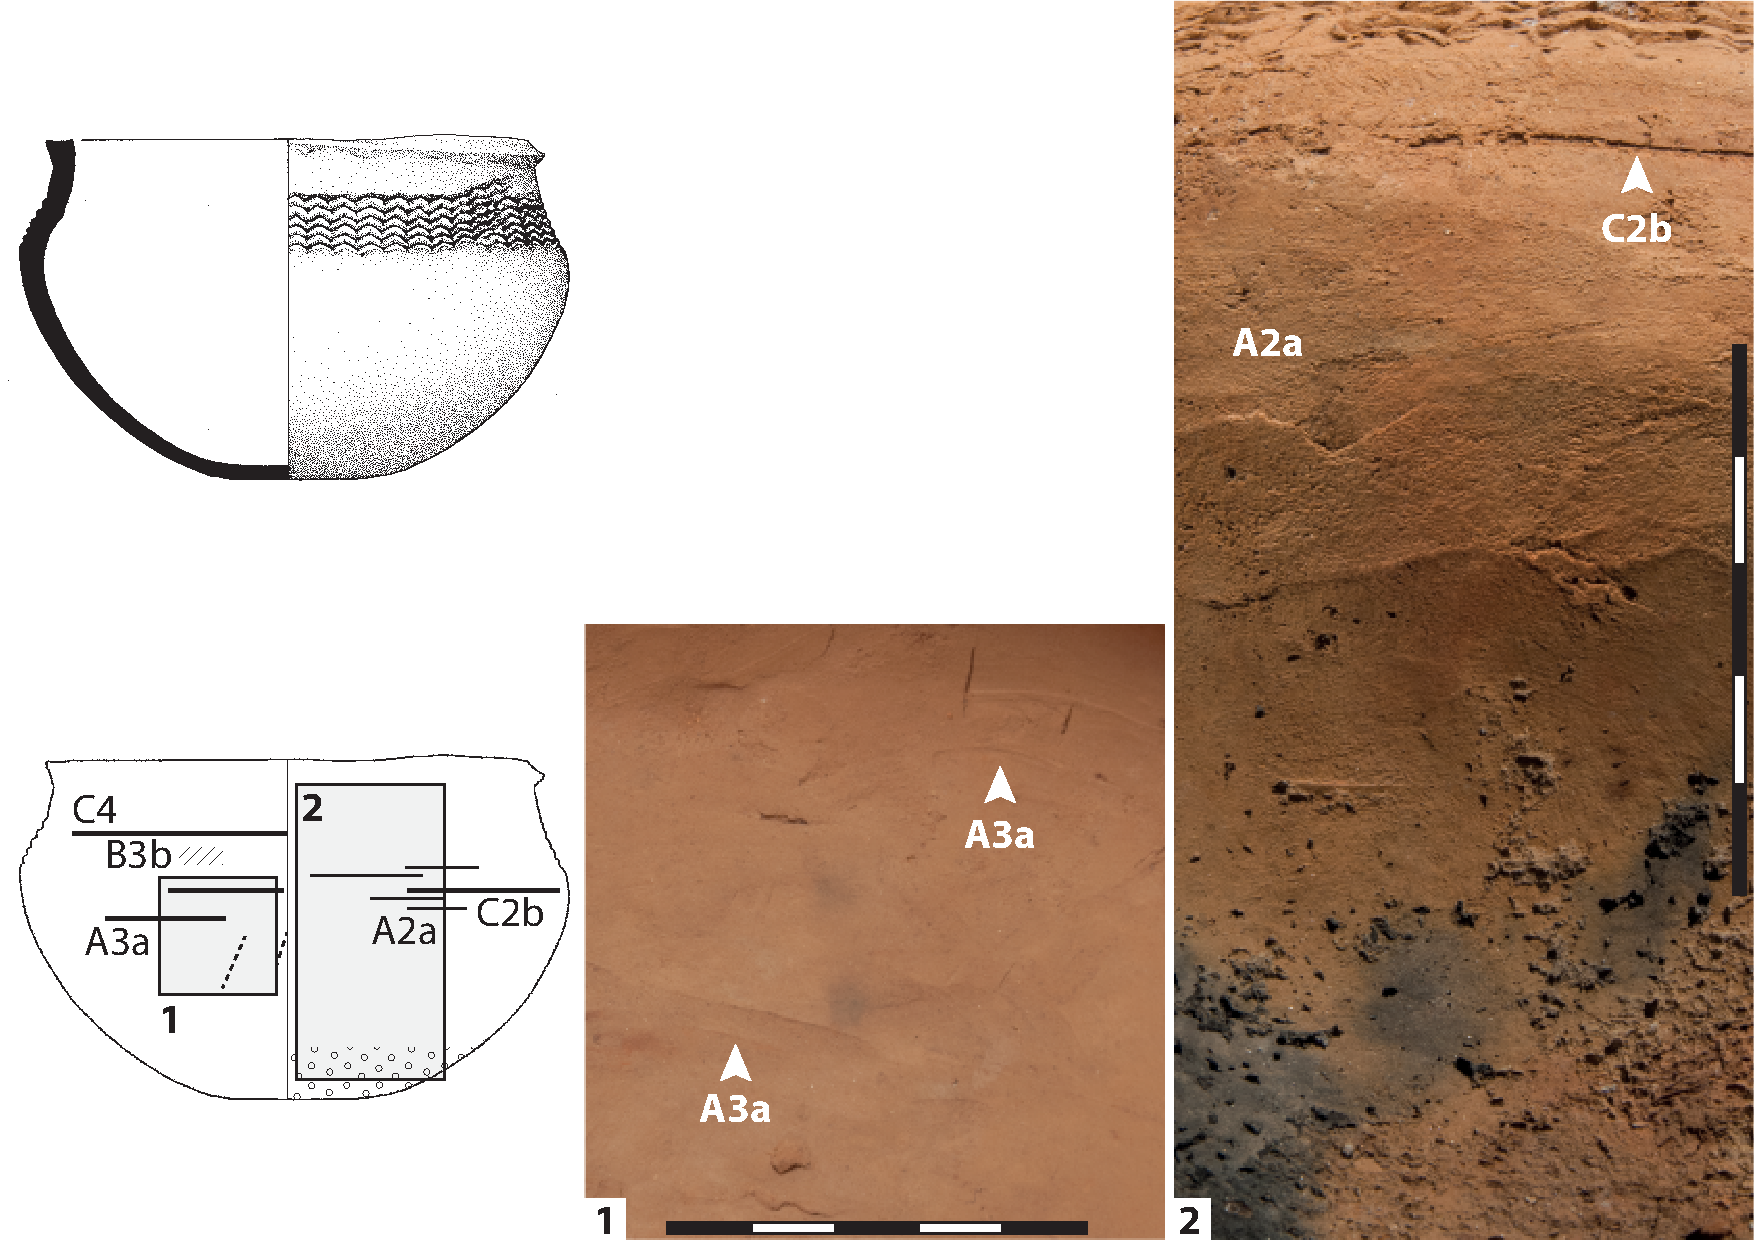
\includegraphics[width = \textwidth]{fig/Abb_Macrotraces/DAM85-503-b.pdf}
		\caption{Dama (Fpl.~222): Obj.~DAM~85/503:2 (Taf.~23.3).}
		\label{DAM85-503-2_Makrospuren}
	\end{subfigure}
	\caption{Makrospuren: Aufnahme und Details.}
	\label{DAM85-503_Makrospuren}
\end{figure*}

Die weiter nördlich, entlang des mittleren bis oberen \mbox{Ubangi} verbreitete, ebenfalls rezente Dama-Gruppe (Kap.~\ref{sec:DAM-Gr}) ist durch zwei Gefäße repräsentiert, deren Herstellung 1985 im eponymen Fundort (Fpl.~222) direkt beobachtet werden konnte.\footnote{Siehe Anm.~\ref{ftn:EthnoToepfereiInVorb}.} Das erste Gefäß ist beim Brand zersprungen. Auffällig sind die vornehmlich horizontalen Brüche (Abb.~\ref{DAM85-503-1_Makrospuren}.3:~D2a) knapp oberhalb des größten Durchmessers, die auf den Aufbau in zwei Abschnitten hinweisen. Außen finden sich lediglich im Bereich knapp unterhalb der größten Gefäßweite einige feine und kurze Glättspuren (A2a). Der kurz ausgeformte Halsbereich weist innen horizontale, eng sitzende, feine Glättriefen auf (A2a). Im Bereich der größten Gefäßweiten finden sich etwa 5--10\,cm lange, zwar entschieden bogenförmige, aber grundsätzlich horizontal ausgerichtete, tiefe Riefen (Abb.~\ref{DAM85-503-1_Makrospuren}.1:~A3a). Unterhalb der größten Weite lassen sich lediglich kurze, diagonal verlaufende und sich stellenweise überlagernde, feine Riefen beobachten (Abb.~\ref{DAM85-503-1_Makrospuren}.2:~A3c). Das Gefäßunterteil ist sehr regelmäßig ausgeformt.	Das zweite, intakt gebliebene Gefäß zeigt auf der Außenseite im Bereich des größten Durchmessers feine horizontale, leicht bogenförmige Glättspuren (Abb.~\ref{DAM85-503-2_Makrospuren}.2:~A2a). Knapp oberhalb des größten Durchmessers befindet sich ein horizontal verlaufender, teilweise überstrichener Grad (Abb.~\ref{DAM85-503-2_Makrospuren}.2:~C2b), der die Grenze zwischen zwei unterschiedlich gefertigten Gefäßteilen markiert. Innen ist der Ansatz des Halses ebenfalls durch einen Grad markiert (C4). Im Bereich des Gefäßbauches finden sich bogenförmige tiefe Glättspuren (Abb.~\ref{DAM85-503-2_Makrospuren}.1:~A3a) und feine, diagonale wirbelähnliche Aufhäufungen von Ton. Im Schulterbereich sind auf der Innenseite einige Eintiefungen (B3b) zu beobachten. Der Gefäßboden ist sehr symmetrisch und gleichmäßig ausgearbeitet. Beide Gefäße weisen Abplatzungen der äußeren Oberfläche im Bereich der Gefäßböden auf. Inwieweit sie darauf zurück zu führen sind, dass die Gefäße in einer kleinen Erdgrube gefertigt wurden und keine konkav geformte \textit{Schablone}, wie ein altes Gefäßfragment, genutzt wurde, muss im Rahmen dieser Betrachtungen offenbleiben.\footnote{Siehe Anm.~\ref{ftn:EthnoToepfereiInVorb}.}

\vspace{1.5em}
\noindent Die beobachteten Makrospuren der untersuchten Gefäße ließen sich in drei Gruppen gliedern (Tab.~\ref{tab:Makrospuren_ChaineOperatoire}). Die Gruppe A bilden Gefäße, die grundsätzlich in einem Arbeitsgang, von unten nach oben aufgebaut wurden und horizontal orientierte Schwankungen der Wandungsdicke (C2a) oder sogar sichtbare, unverstrichene Wülste aufweisen (siehe Abb.~\ref{DON85-101-71_Makrospuren}.1). Weitere Indizien, die für die Zuweisung zu dieser Gruppe herangezogen wurden, sind ein diagonal verlaufender, interner Aufbau der Bruchflächen gemäß \textcite[140 Abb.~8.b]{Lindahl.2010} und vornehmlich horizontale, durch den Gefäßkörper laufende Bruchlinien (D2a) oder Risse (D3a). Gruppe B zeichnet sich vornehmlich durch Hinweise darauf aus, dass der Aufbau vom Rand zum Boden hin und in zwei Teilen erfolgte. Beobachtungen, wonach der Boden mutmaßlich erst zum Ende des Arbeitsprozesses geschlossen oder ausgeformt wurde, lassen sich aus Verengungen des Gefäßdurchmessers und damit einhergehenden vertikal laufenden ziehharmonikaartigen \textit{Rippen} (C1) ableiten, die sich vor allem oberhalb des Bodenansatzes finden. Ebenfalls können buckelartige, isolierte Verdickungen der Gefäßboden (C3a) oder eine drastische Ausdünnung des Boden (C3b) als Indizien dafür gewertet werden, dass der Boden ausschließlich mit vorhandenem Material geschlossen beziehungsweise ausgeformt wurde. Die beobachteten buckelartigen Verdickungen des Gefäßbodens fallen häufig mit radial laufenden beziehungsweise sternförmigen Rissen zusammen, die andeuten, dass der Boden nicht aus einem Stück geformt wurde (siebe Abb.~\ref{MUN87-1-0-2-1-3_Makrospuren}--b). Des Weiteren lässt sich bei Gefäßen der Gruppe B ein lagiger Aufbau der in den Bruchflächen sichtbaren, inneren Struktur des Scherbens ausmachen (ebd. 140 Abb.~8.c--d). Zudem können vornehmlich diagonal durch den Gefäßkörper laufende Brüche (D2b) und Risse (D3b) als Indikatoren für die Zuweisung zu Gruppe B gelten. Die Gefäße der Gruppe C zeichnen sich durch äußerst regelmäßig geformte, runde Gefäßunterteile beziehungsweise Böden aus. Die Unterteile haben häufig einen stark komprimierten und dichten Scherben. Oft sind die Gefäße dieser Gruppe in zwei Teilen hergestellt, mit einem deutlich sicht- oder fühlbaren Übergang. 


\section{Scherben und \textit{Fabric}}\label{sec:Herstellung2_Fabric}

Im Rahmen einer ersten Testreihe wurden 2012 eine aus 25 Keramikscherben bestehende Auswahl aus dem Inneren Kongobecken angeschliffen, die für spätere Analysen separiert worden waren und einen groben chronologischen wie regionalen Querschnitt seines Untersuchungsraums widerspiegeln.\footnote{Die Testserie aus dem Inneren Kongobecken beinhaltete Scherben der Fundplätze Iyonda (Fpl.~8), Mbandaka (Fpl.~10), Bokele (Fpl.~14), Nkile (Fpl.~17), Bokuma (Fpl.~18), Ikenge (Fpl.~20), Longa (Fpl.~24), Benkombo (Fpl.~24a), Imbonga (Fpl.~43), Bonkake (Fpl.~47) und Mondjo (Fpl.~133). Die Anschliffe wurden in den Jahren 2012--13 in der Forschungsstelle Afrika des Instituts für Ur- und Frühgeschichte der Universität zu Köln auf einer \textit{Wirtz TE 200} Schleifmaschine mittels Diamant-Schleifscheiben mit einer Körnung von 40\,$\mu$m angefertigt. Die Anschliffe wurden anschließend auf einem \textit{Epson GT-15000}-Flachbettscanner bei einer Auflösung von 1200\,dpi eingescannt. Theoretisch wurde dadurch eine Auflösung von 21,2\,$\mu$m je Pixel erzielt. Obschon der Scanner technisch höhere Auflösungen anbot, wiesen entsprechende Tests keine weiteren diagnostischen Merkmale, sondern lediglich ein höheres Bildrauschen und Kompressionsartefakte auf.\label{ftn:Anschliffe2012_ICB_Fpl}} Zusätzlich zu diesem von \textcite{Wotzka.1995} bereits stilistisch angesprochenen Material wurde auch eine Stichprobe von 20 Scherben aus dem nordwestlichen Kongobecken angeschliffen, die einen ersten Einblick in die regionale Variation der technischen Eigenschaften der Keramik des Arbeitsgebietes liefern sollte. Die Gefäßeinheiten aus dem Inneren Kongobecken zeigten eine auffallende Homogenität.\footnote{Lediglich die Stilgruppen der \textit{Tshuapa-Tradition} (Kap.~\ref{sec:ICB_StilGrDatierungen}) umfassen auch Gefäße mit höheren Anteilen von Quarzsand, die von \textsc{Wotzka} (1995: 175, 181, 186, 197) als intentionelle Zuschläge im Sinne einer Magerung angesehen werden. GE mit Sandmagerung machen bis zu 56\,\% der entsprechenden Stile aus (ebd. 181).\label{ftn:Sandmagerung}} Etwa 84\,\% ließen sich einer Gruppe zuweisen, die im späteren Bearbeitungsprozess als \textit{Fabric} 1 konzeptualisiert wurde (Tab.~\ref{tab:Fabrics_Bilder}: 1a--e). Diese Testreihe bildete den Ausgangspunkt für die hier beschriebene, systematische Untersuchung.

Die Materialaufnahme umfasste eine Beschreibung technischer Parameter der keramischen Inventare (Kap.~\ref{sec:AufnahmeTechnologie}), die als Grundlage für eine spätere Systematisierung und Gruppenbildung diente. Zur Gliederung der an den individuellen Scherben beobachteten Variabilität der Eigenschaften der genutzten Tone und deren Aufarbeitung wurde das Konzept des \textit{Fabric} herangezogen \parencite[ebd. 49, 54--56][38--51]{Riemer.2011}.\footnote{Das hier genutzte Verständnis von \textit{Fabric} lehnt sich stark an das von \textcite[49]{Lange.2006} verwendete Konzept an, welches \textit{Fabric} als \enquote{Sammelbezeichnung für alle wichtigen chemischen und physikalischen Eigenschaften des Tones und der nichtplastischen Bestandteile} versteht und sich am besten mit \enquote{Rezept} übersetzen ließe. Im Fall der untersuchten Gefäßkeramik wurde die grundsätzliche Brennfarbe der genutzten Tone in die Klassifikation einbezogen \parencite[siehe][34]{Nordstrom.1972}. Eine Zonierung der Färbung \parencite[siehe][90 Abb.~4-1]{Clist.20042005}, die sich abhängig von Dauer und Intensität des Brandes ergibt, wurde lediglich als nachrangiges Kriterium aufgenommen. Bei der Durchsicht des Materials wurde deutlich, dass die Färbung der Stücke in einem Maße heterogen ist, dass vor dem Licht der universal praktizierten offenen Haufenbrände \parencite[siehe][217 Karte~17]{Drost.1967} bei dem vorliegenden zerscherbten Material zu selten für die gesamte GE gültige Ansprachen gemacht werden können. Der Keramikbrand im Töpfereizentrum von Ikenge am Ruki wurde ausführlich von \textcite[402--404; 422\,f. Abb.~16--18]{Eggert.1980c} und \textcite{Wotzka.1991} beschrieben. Grundsätzlichere Arbeiten zum Keramikbrand stammen von \textcite{Gosselain.1992b} und \textcite{LivingstoneSmith.2001} sowie \textcite{LundRasmussen.2012}, während \textcite[146 Abb.~17]{Lindahl.2010} den Brand von Gefäßen im südlichen Afrika beschreiben. Für die europäische Archäologie sei an dieser Stelle lediglich schlaglichtartig auf die Arbeit von \textcite{Ther.2011} zum Brand von spätbronzezeitlicher Keramik aus Tscheschien verwiesen.\label{ftn:Keramikbrand}} \textit{Fabrics} sind in der vorliegenden Arbeit jedoch nicht als bloße Beschreibung der technischen Eigenschaften anzusehen, sondern spiegeln ein wiedererkennbares Konzept vergangener Entscheidungsprozesse im Bereich der Rohmaterialbeschaffung und -aufbereitung wider (siehe Kap.~\ref{sec:Herstellung_ChaineOperatoire}). Sie bilden folglich eine kulturhistorisch auswertbare Entität im Zusammenhang mit der Analyse der prähistorischen Keramik des Arbeitsgebietes.\footnote{Radiometrische Untersuchungen der Gefäße, wie sie von \textcites{LivingstoneSmith.2007d}{LivingstoneSmith.2010c} durchgeführt wurden, konnten im Rahmen dieser Studie nicht umgesetzt werden. Auch dezidierte Untersuchungen zur Mineralogie, Korngrößenverteilung und zum Chemismus der Stücke sowie von Tonproben aus der Region ließen sich nicht realisieren (ebd. 24).}

Insgesamt konnte die beobachtete Variabilität zu neun unterschiedlichen \textit{Fabrics} zusammengefasst werden, wobei sich unter Berücksichtigung aller Untergruppen 27 unterscheidbare Variationen ergaben (Tab.~\ref{tab:Fabrics_Bilder}). Ausgehend von den an Anschliffen\footnote{Es wurden insgesamt 381 Anschliffe hergestellt, dies entspricht 4,5\,\% der untersuchten GE.} erarbeiteten Kriterien erfolgte für die weiteren Inventare die Ansprache des \textit{Fabrics} direkt bei der Aufnahme. Insgesamt konnte für 91\,\% aller Scherben der \textit{Fabric} sicher angesprochen werden. 

Aus den Beobachtungen der ersten Testreihe an Keramik des Inneren wie nordwestlichen Kongobeckens wurde eine Arbeitshypothese formuliert, nach der die fehlende Heterogenität der \textit{Fabrics} im Inneren Kongobecken mit der von \textcite[58--210]{Wotzka.1995} auf Basis morphologischer und ornamentaler Kriterien erarbeiteten \textit{Äquator-Co-Tradition} in Zusammenhang steht.

\end{multicols}
%\afterpage{%
\clearpage
\begin{footnotesize}
{\sffamily
\begin{longtable}{@{}m{.3\textwidth}m{.3\textwidth}m{.05\textwidth}m{.27\textwidth}@{}}
\toprule
\textbf{Außenseite/Oberfläche} & \textbf{Anschliff (Profil)} & \textbf{\textit{Fabric}} & \textbf{Kurzbeschreibung} \\
\midrule
\endhead

\includegraphics[width=.3\textwidth, page = 1]{tbl/Tab_Fabrics/x_fabrics_scales.pdf} & 
\includegraphics[width=.3\textwidth, page = 2]{tbl/Tab_Fabrics/x_fabrics_scales.pdf} &  &  \\
\bottomrule
\caption{Keramik: Übersicht über die \textit{Fabrics}.}
\label{tab:Fabrics_Bilder}
\endfoot
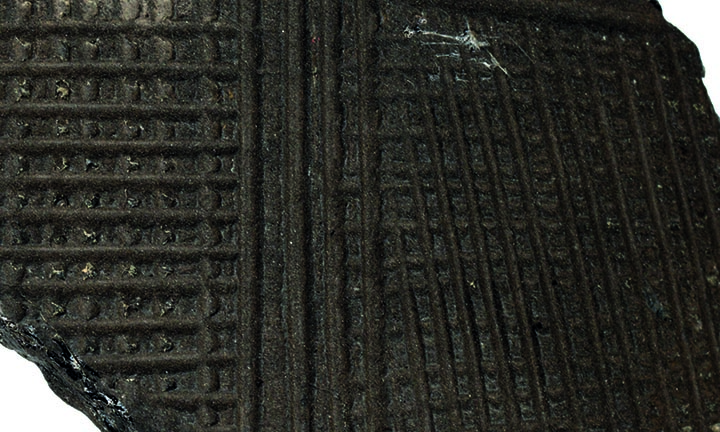
\includegraphics[width=.3\textwidth]{tbl/Tab_Fabrics/PIK87-1-8-6_aussen_5cm.jpg} & 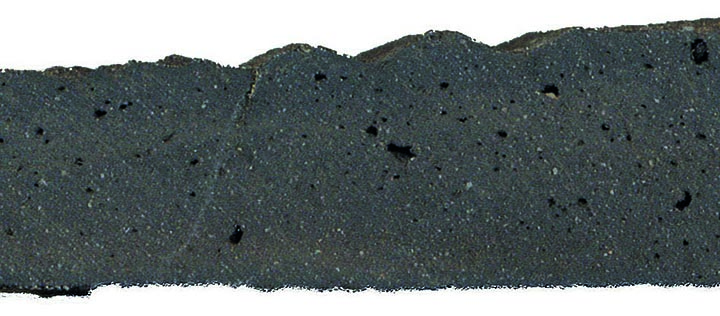
\includegraphics[width=.3\textwidth]{tbl/Tab_Fabrics/PIK87-1I9-1_2cm.jpg} & 1a & Der \textit{Scherben} lässt makroskopisch keine nichtplastischen Partikel erkennen und ist im Anschliff komplett schwarz (Obj.:~PIK~87/1/I-9:1). \\
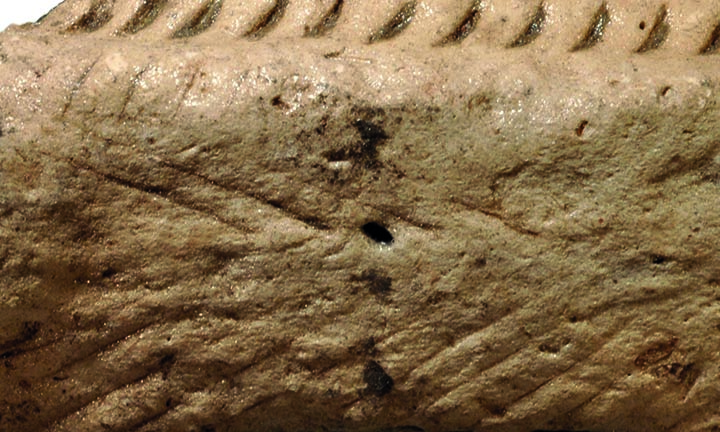
\includegraphics[width=.3\textwidth]{tbl/Tab_Fabrics/MBA_201-12_5cm.jpg} & 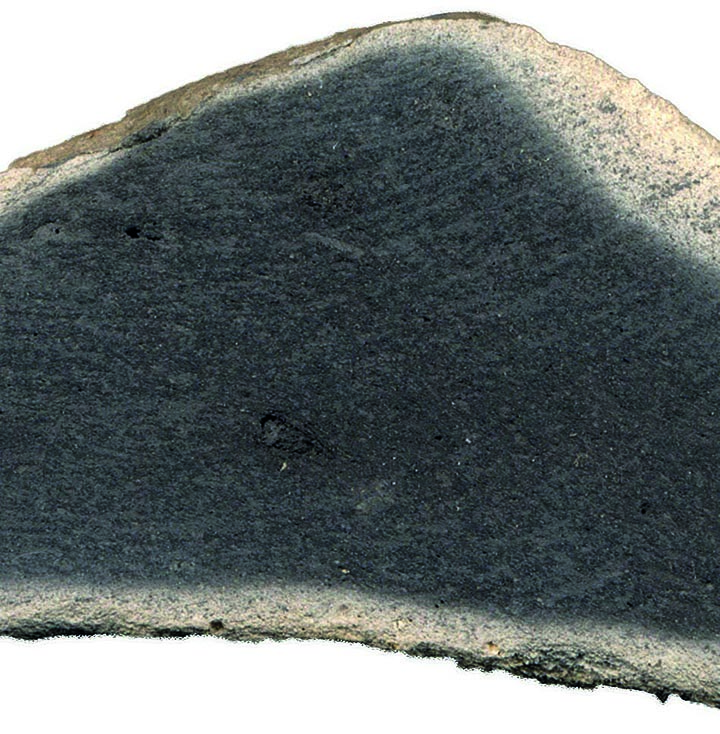
\includegraphics[width=.3\textwidth]{tbl/Tab_Fabrics/MBA_201-12_2cm.jpg} & 1b & Wie 1a, der \textit{Scherben} ist randlich weißbrennend oxidiert. Der Bereich der Oxidation lässt sich deutlich vom dunklen Kern abgrenzen (Obj.:~MBA~201:12). \\
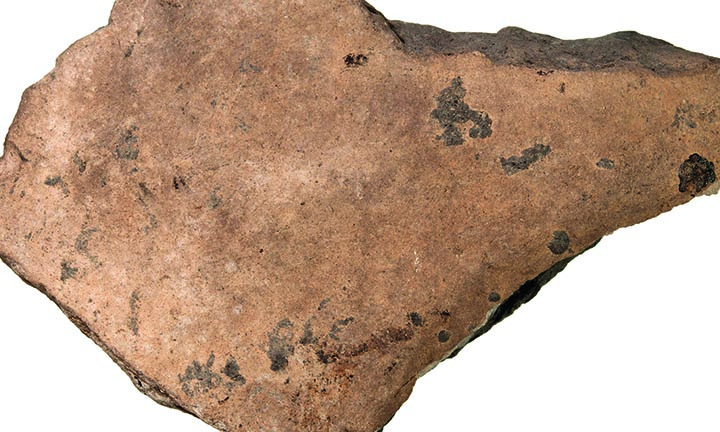
\includegraphics[width=.3\textwidth]{tbl/Tab_Fabrics/MSN87-101-142_5cm.jpg} & 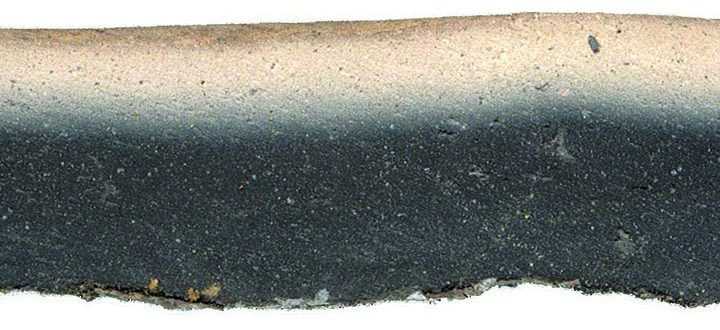
\includegraphics[width=.3\textwidth]{tbl/Tab_Fabrics/MSN87-101-142_2cm.jpg} & 1c & Wie 1a, der \textit{Scherben} ist nur auf einer Seite deutlich oxidiert, während auf der Gegenseite keine Oxidation sichtbar ist. Der oxidierte Bereich grenzt sich scharf vom dunklen Kern ab (Obj.:~MSN~87/101:142).\vspace{1em} \\
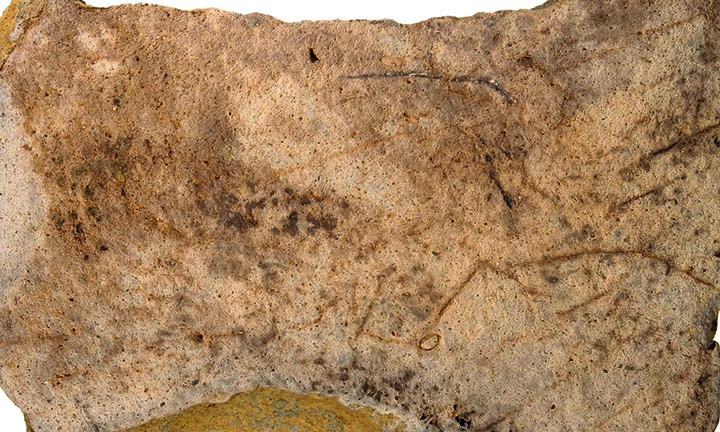
\includegraphics[width=.3\textwidth]{tbl/Tab_Fabrics/BTW87-101-43_5cm.jpg} & 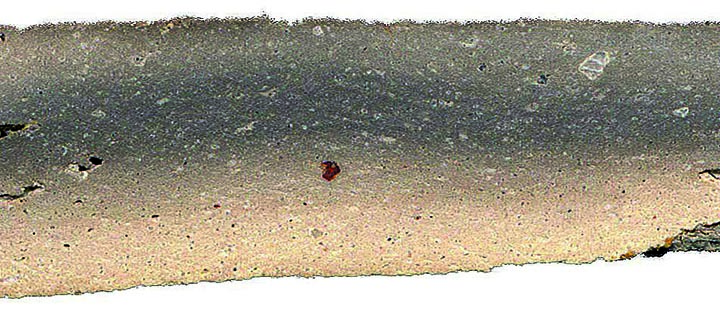
\includegraphics[width=.3\textwidth]{tbl/Tab_Fabrics/BTW87-101-43_2cm.jpg} & 1d & Wie 1a, der \textit{Scherben} ist größtenteils, bis auf einen teilweise nur blassen, dunklen Restkern oxidiert. Die oxidierte Zone geht fließend in den Restkern über (Obj.:~BTW~87/101:43). \\
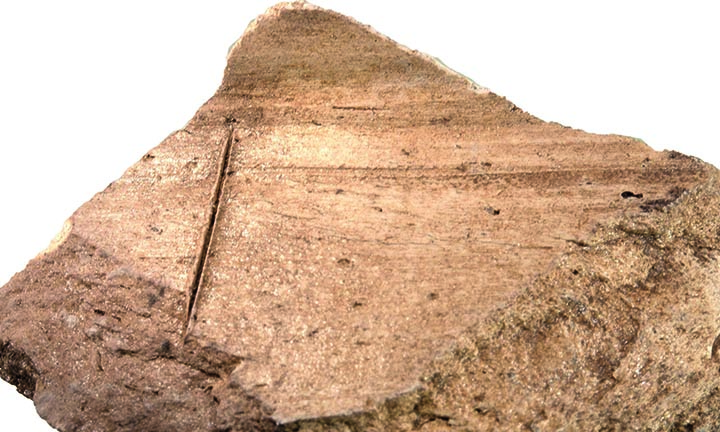
\includegraphics[width=.3\textwidth]{tbl/Tab_Fabrics/IKE81-1-12_5cm.jpg} & 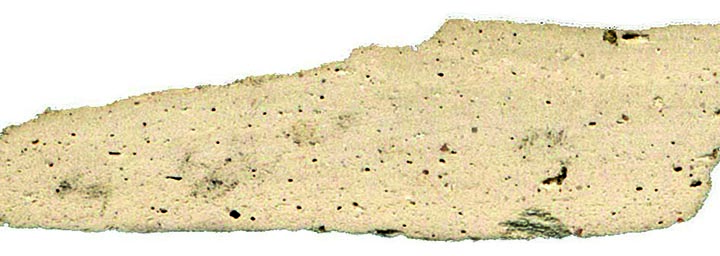
\includegraphics[width=.3\textwidth]{tbl/Tab_Fabrics/IKE81-1-12_2cm.jpg} & 1e & Wie 1a, der \textit{Scherben} ist vollständig durchoxidiert, ein Kern ist nicht mehr zu beobachten (Obj.:~IKE~81/1:12). \\
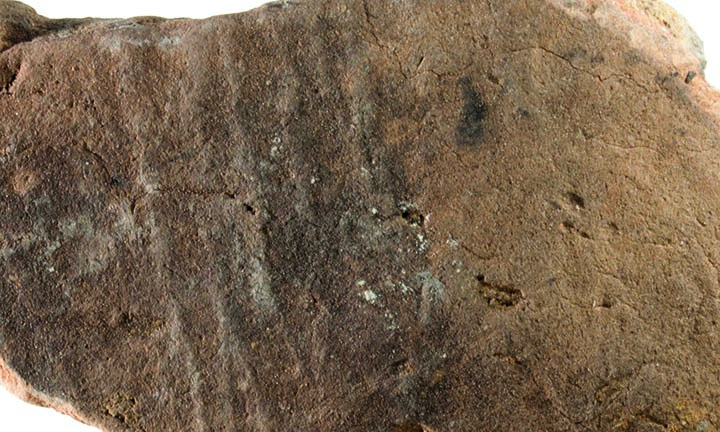
\includegraphics[width=.3\textwidth]{tbl/Tab_Fabrics/BKE81-2-2-9_5cm.jpg} & 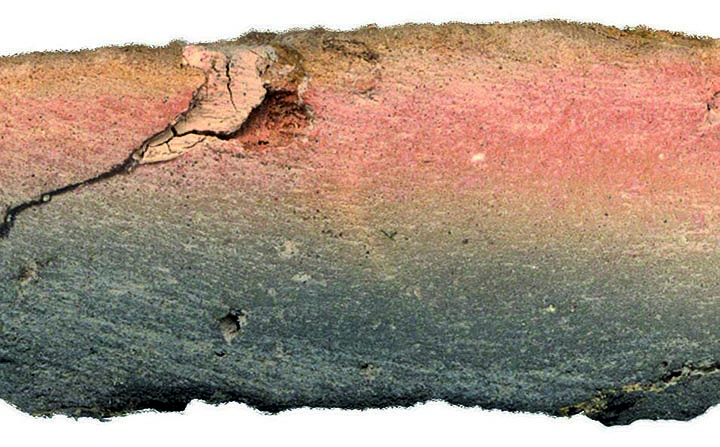
\includegraphics[width=.3\textwidth]{tbl/Tab_Fabrics/BKE81-2-2-9_2cm.jpg} & 2a & Wie 1d, ist der genutzte Ton rotbrennend. Ein Restkern ist noch sichtbar (Obj.:~BKE~81/2-2:9). \\
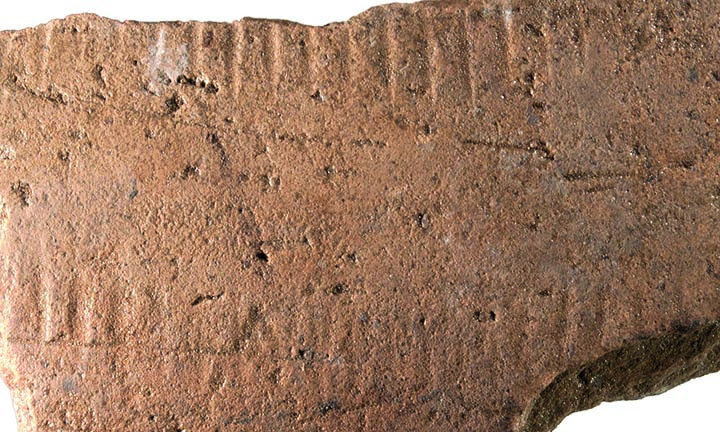
\includegraphics[width=.3\textwidth]{tbl/Tab_Fabrics/IMB81-3-2_11_5cm.jpg} & 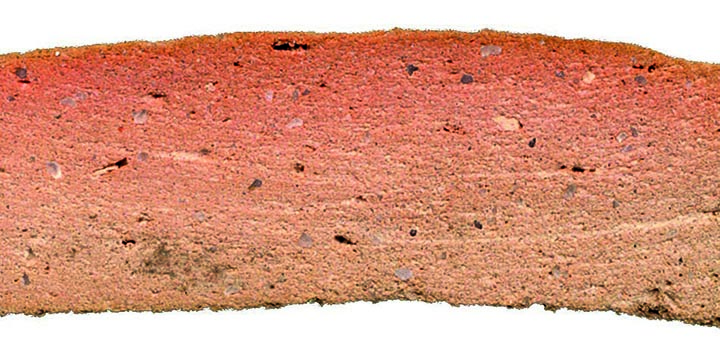
\includegraphics[width=.3\textwidth]{tbl/Tab_Fabrics/IMB81-3-2_11_2cm.jpg} & 2b & Wie 2a, der \textit{Scherben} ist vollständig rotbrennend durchoxidiert (Obj.:~IMB~81/3-2:11). \\
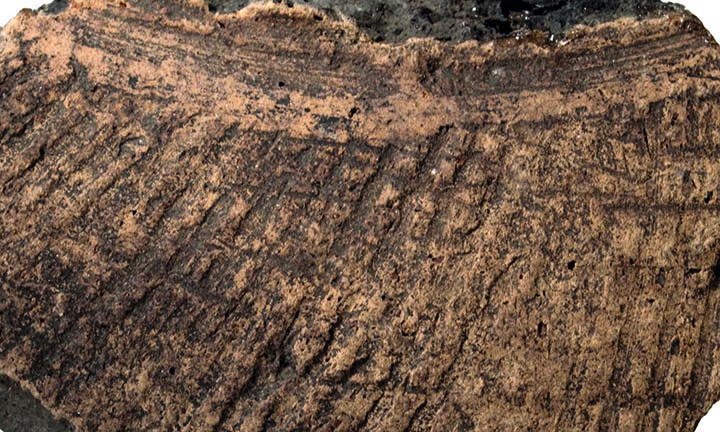
\includegraphics[width=.3\textwidth]{tbl/Tab_Fabrics/PIK87-1-2-225_5cm.jpg} & 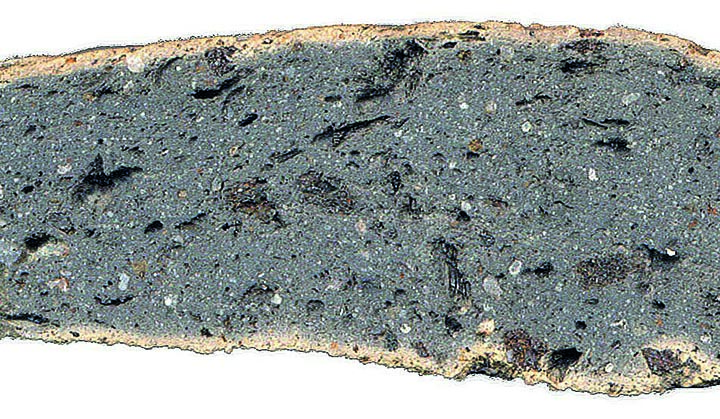
\includegraphics[width=.3\textwidth]{tbl/Tab_Fabrics/PIK87-1-2-225_2cm.jpg} & 3a & Der \textit{Scherben} enthält bis zu 20~\% nichtplastische Partikel der Größenklassen \textit{medium} bis \textit{coarse} (250--1000\,$\mu$m) und zeigt innen wie außen eine schmale, scharf abzugrenzende, weißbrennende Oxidationszone. In geringem Maße finden sich ausgebrannte Reste organischer Partikel (Obj.:~PIK~87/1-2:225). \\
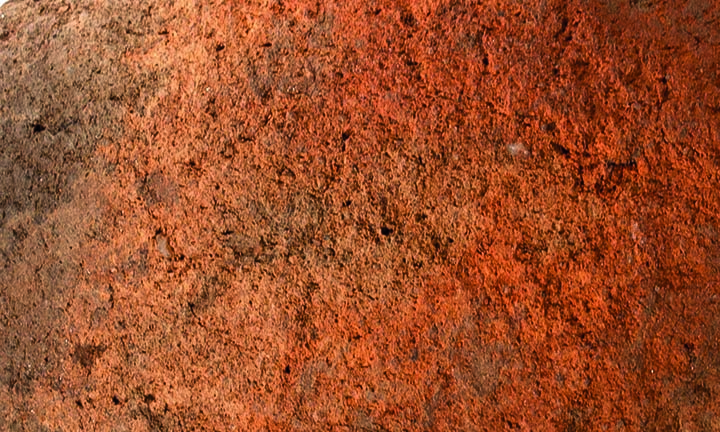
\includegraphics[width=.3\textwidth]{tbl/Tab_Fabrics/PDM87-102-20_5cm.jpg} & 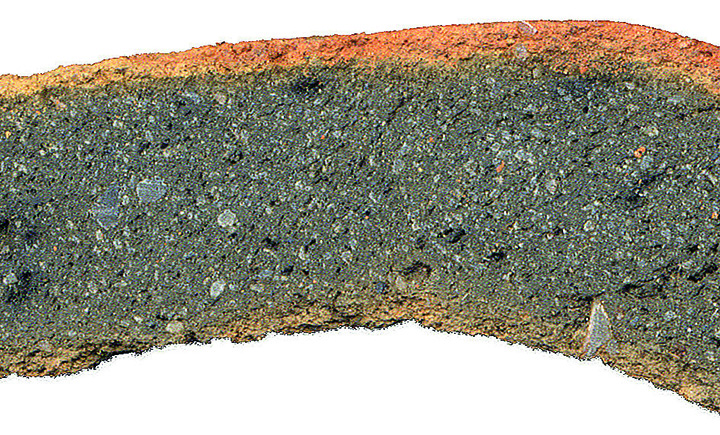
\includegraphics[width=.3\textwidth]{tbl/Tab_Fabrics/PDM87-102-20_2cm.jpg} & 3b & Wie 3a, die Brennfarbe des Scherbens ist rot (Obj.:~PDM~87/102:20). \\
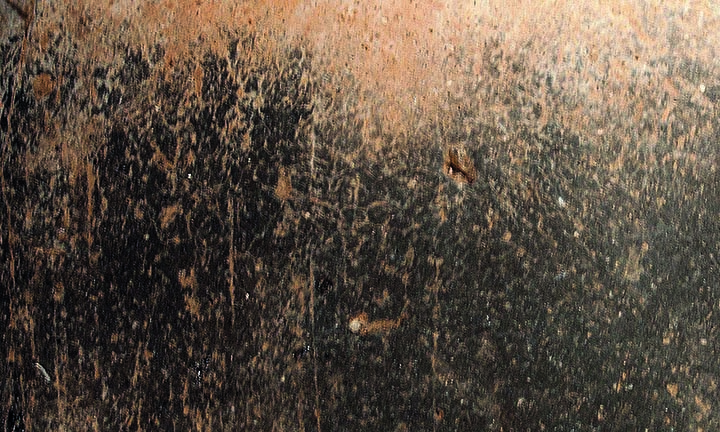
\includegraphics[width=.3\textwidth]{tbl/Tab_Fabrics/BYN87-101-10_5cm.jpg} & 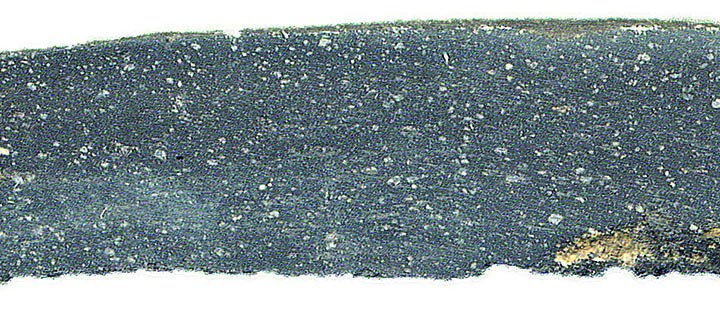
\includegraphics[width=.3\textwidth]{tbl/Tab_Fabrics/BYN87-101-10_2cm.jpg} & 3c & Wie 3a, der \textit{Scherben} zeigt keine randliche Oxidation. Hinweise auf ausgebrannte Organik sind sehr selten (Obj.:~BYN~87/101:10). \\
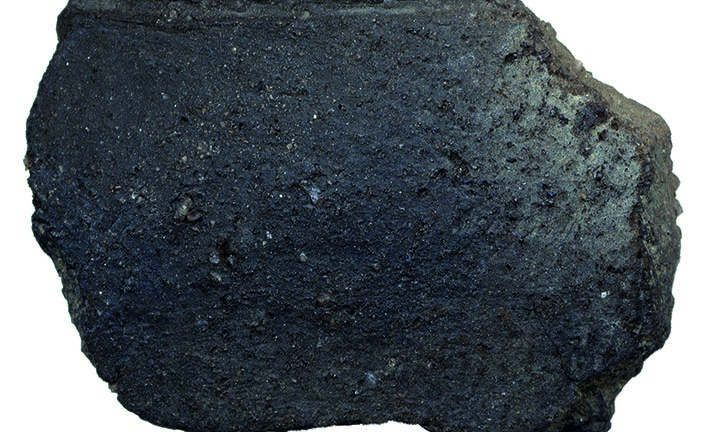
\includegraphics[width=.3\textwidth]{tbl/Tab_Fabrics/PIK87-1-8-1_5cm.jpg} & 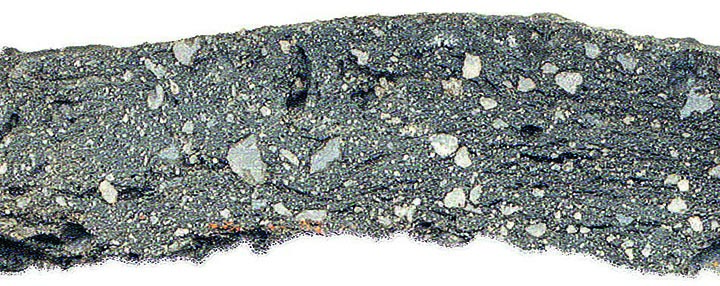
\includegraphics[width=.3\textwidth]{tbl/Tab_Fabrics/PIK87-1-8-1_2cm.jpg} & 4a & Der \textit{Scherben} enthält bis zu 40~\% nichtplastischer Partikel (kantiger Quarz) der Größenklassen \textit{coarse} bis \textit{very coarse} (500--2000\,$\mu$m). Im Anschliff ist er komplett grau bis schwarz (Obj.:~PIK~87/1-8:1).\vspace{1em} \\
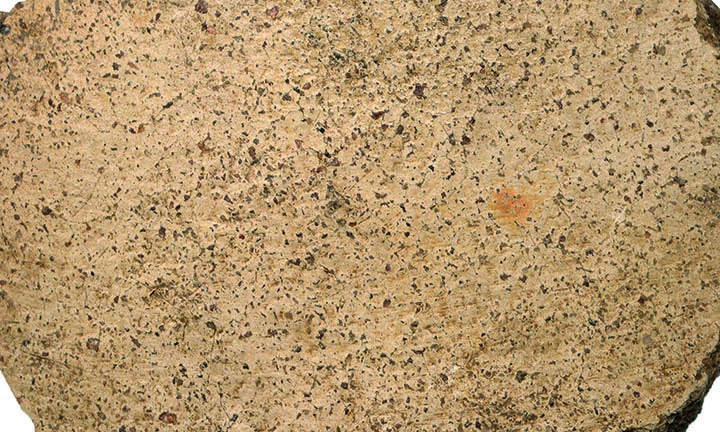
\includegraphics[width=.3\textwidth]{tbl/Tab_Fabrics/DON85-102-1_5cm.jpg} & 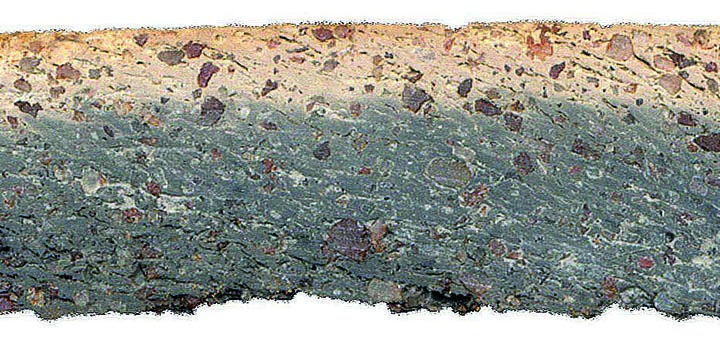
\includegraphics[width=.3\textwidth]{tbl/Tab_Fabrics/DON85-102-1_2cm.jpg} & 4b & Wie 4a, teilweise enthält der \textit{Scherben} rötliche, leicht abgerundete Quarzkörner. Regelhaft weist er eine gut abzugrenzende, weißbrennende Oxidationszone auf (Obj.:~DON~85/102:1).\vspace{1em} \\
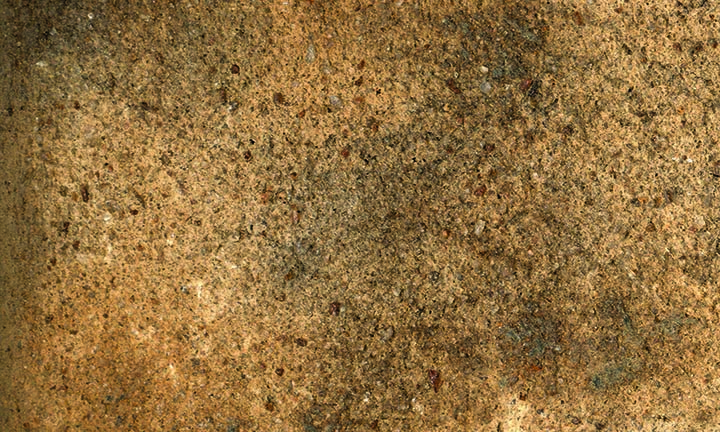
\includegraphics[width=.3\textwidth]{tbl/Tab_Fabrics/MBN85-101-60_5cm.jpg} & 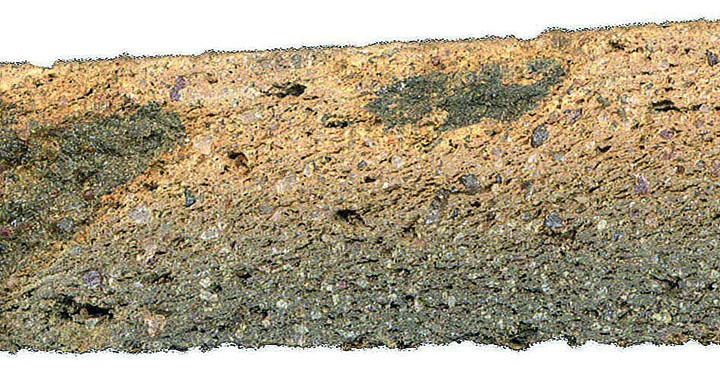
\includegraphics[width=.3\textwidth]{tbl/Tab_Fabrics/MBN85-101-60_2cm.jpg} & 4c & Wie 4a, der \textit{Scherben} ist bis auf einen meist schwachen Restkern deutlich weißbrennend oxidiert. Die Grenze zum Restkern ist nur schwach ausgeprägt (Obj.: MBN 85/101:60). \\
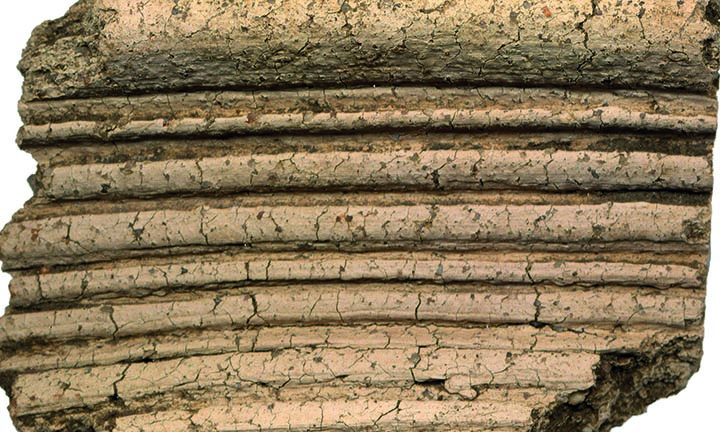
\includegraphics[width=.3\textwidth]{tbl/Tab_Fabrics/MLB85-101-22_5cm.jpg} & 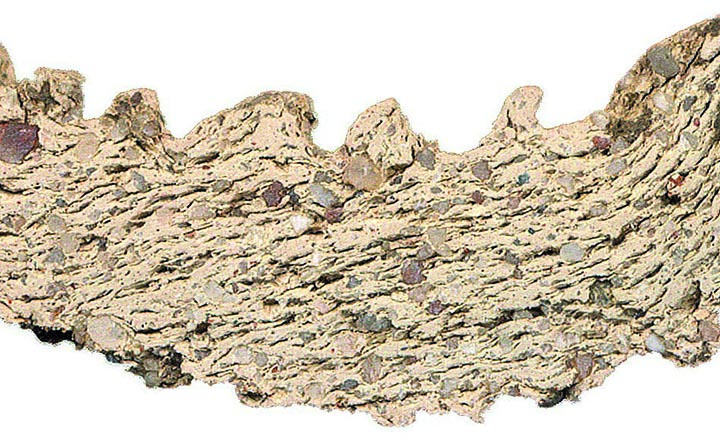
\includegraphics[width=.3\textwidth]{tbl/Tab_Fabrics/MLB85-101-22_2cm.jpg} & 4d & Wie 4a, der \textit{Scherben} ist vollständig weißbrennend durchoxidiert (Obj.:~MLB~85/101:22). \\
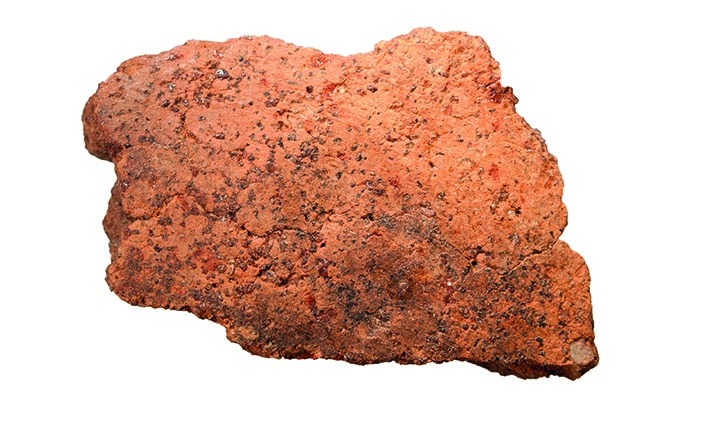
\includegraphics[width=.3\textwidth]{tbl/Tab_Fabrics/MTB85-101-101_5cm.jpg} & 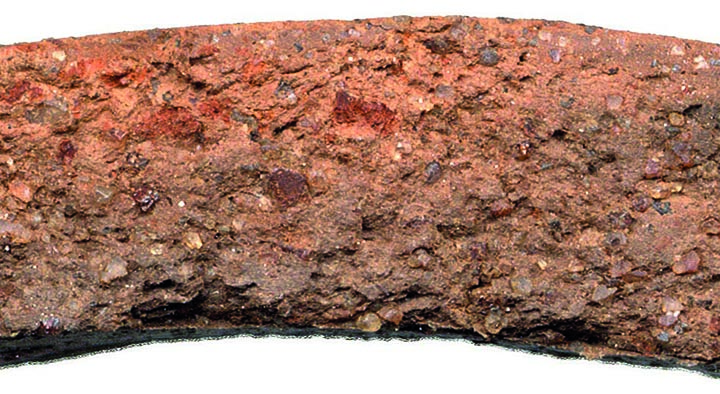
\includegraphics[width=.3\textwidth]{tbl/Tab_Fabrics/MTB85-101-101_2cm.jpg} & 5a & Wie 4a, der \textit{Scherben} ist vollständig rotbrennend oxidiert (Obj.:~MTB~85/101:101). \\
\includegraphics[width=.3\textwidth]{tbl/Tab_Fabrics/DON85-102-123_5cm.jpg} & \includegraphics[width=.3\textwidth]{tbl/Tab_Fabrics/DON85-102-123_2cm.jpg} & 5b & Wie 5a, der \textit{Scherben} ist bis auf einen nur schwach abzugrenzenden, dunklen Restkern rotbrennend oxidiert (Obj.:~DON~85/102:123). \\
\includegraphics[width=.3\textwidth]{tbl/Tab_Fabrics/OUE87-102-49_5cm.jpg} & \includegraphics[width=.3\textwidth]{tbl/Tab_Fabrics/OUE87-102-49_2cm.jpg} & 5c & Wie 5a, der \textit{Scherben} weist eine scharf abzugrenzende rotoxidierte Zone auf (Obj.:~OUE~87/102:49). \\
\includegraphics[width=.3\textwidth]{tbl/Tab_Fabrics/SID85-101-2_5cm.jpg} & \includegraphics[width=.3\textwidth]{tbl/Tab_Fabrics/SID85-101-2_2cm.jpg} & 6a & Der \textit{Scherben} enthält bis zu 40~\% kantigem Quarz der Größenklassen \textit{fine} bis \textit{very coarse} (125--2000\,$\mu$m) sowie auffällig glimmerartiges Material (Obj.: SID 85/101:2). \\
\includegraphics[width=.3\textwidth]{tbl/Tab_Fabrics/KOU85-101-59_5cm.jpg} & \includegraphics[width=.3\textwidth]{tbl/Tab_Fabrics/KOU85-101-59_2cm.jpg} & 6b & Wie 6b, die Farbe des \textit{Scherbens} schwankt zwischen rot, braun und grau (Obj.:~KOU~85/101:59). \\
\includegraphics[width=.3\textwidth]{tbl/Tab_Fabrics/BNA87-101-3_5cm.jpg} & \includegraphics[width=.3\textwidth]{tbl/Tab_Fabrics/BNA87-101-3_2cm.jpg} & 7a & Der \textit{Scherben} enthält bis zu 10~\% Quarzkörner der Größenklassen \textit{fine} bis \textit{coarse} (125--1000\,$\mu$m). Das Stück ist komplett rotbrennend durchoxidiert (Obj.:~BNA~87/101:3).\vspace{1em} \\
\includegraphics[width=.3\textwidth]{tbl/Tab_Fabrics/BMS87-101-1_5cm.jpg} & \includegraphics[width=.3\textwidth]{tbl/Tab_Fabrics/BMS87-101-1_2cm.jpg} & 7b & Wie 7a, der \textit{Scherben} enthält neben Quarzkörnern auch häufig abgerundete, an Laterit erinnernde Partikel der Größenklassen \textit{coarse} bis \textit{very coarse} (500--2000\,$\mu$m). (Obj.:~BMS~87/101:1). \\
\includegraphics[width=.3\textwidth]{tbl/Tab_Fabrics/MBK85-101-81_5cm.jpg} & \includegraphics[width=.3\textwidth]{tbl/Tab_Fabrics/MBK85-101-81_2cm.jpg} & 7c & Wie 7a, der \textit{Scherben} enthält neben Quarz und kleineren Stücken lateritartigen Materials auch eine an Glimmer erinnernde Fraktion feiner Partikel (Obj.:~MBK~85/101:81).\vspace{1em} \\
\includegraphics[width=.3\textwidth]{tbl/Tab_Fabrics/MLB85-1-1-87_5cm.jpg} & \includegraphics[width=.3\textwidth]{tbl/Tab_Fabrics/MLB85-1-1-87_2cm.jpg} & 7d & Wie 7a, der \textit{Scherben} zeigt eine von einem grauen bis schwarzen Kern scharf abgrenzbare, rotbrennende Oxidation (Obj.:~MLB~85/1-1:87).\vspace{1em} \\
\includegraphics[width=.3\textwidth]{tbl/Tab_Fabrics/MND85-101-21_5cm.jpg} & \includegraphics[width=.3\textwidth]{tbl/Tab_Fabrics/MND85-101-21_2cm.jpg} & 7e & Wie 7d, der \textit{Scherben} zeigt einen homogenen grauen Kern mit einer scharf abgegrenzten, nur wenige Millimeter tief eindringenden, rotbrennenden Oxidation. Neben feinen Quarzkörnern enthält er lateritartige Partikel der Größenklassen \textit{coarse} bis \textit{very coarse} (500--2000\,$\mu$m) (Obj.:~MND~85/101:21).\vspace{1em} \\
\includegraphics[width=.3\textwidth]{tbl/Tab_Fabrics/KPT85-101-9_5cm.jpg} & \includegraphics[width=.3\textwidth]{tbl/Tab_Fabrics/KPT85-101-9_2cm.jpg} & 8a & Der \textit{Scherben} enthält neben Quarzkörnern, Resten ausgebrannter Organik sowie teilweise glimmerartigen Partikeln auch eine Fraktion Schamott. Die Zusammensetzung der nichtplastischen Partikel ist mit Bezug auf Art, Größe und Dichte sehr heterogen (Obj.:~KPT~85/101:9). \\[1em]
\includegraphics[width=.3\textwidth]{tbl/Tab_Fabrics/SUN87-101-72_5cm.jpg} & \includegraphics[width=.3\textwidth]{tbl/Tab_Fabrics/SUN87-101-72_2cm.jpg} & 9a & Der Scherben enthält ausschließlich Schamott der Größenklas"-sen \textit{coarse} bis \textit{very coarse} (500--2000\,$\mu$m). Ein grauer bis schwarzer Kern wird von einer scharf ab"-zu"-gren"-zen"-den, rand"-lichen, weiß"-brennenden Oxi"-dations"-zone umschlossen (Obj.:~SUN~87/101:72).\vspace{1em} \\
\includegraphics[width=.3\textwidth]{tbl/Tab_Fabrics/SUN87-101-87_5cm.jpg} & \includegraphics[width=.3\textwidth]{tbl/Tab_Fabrics/SUN87-101-87_2cm.jpg} & 9b & Wie 9a, der \textit{Scherben} ist vollständig weißbrennend durchoxidiert (Obj.:~SUN~87/101:87) \\
\end{longtable}
}
\end{footnotesize}
%}
\clearpage
\begin{multicols}{2}
\raggedcolumns
\noindent

Während sich im nordwestlichen Kongobecken durchaus sehr ähnliche und auch identische \textit{Fabrics} (Tab.~\ref{tab:Fabrics_Bilder}: \textit{Fabric} 1) fanden, die der Arbeitshypothese folgend mit der Keramik des Inneren Kongobeckens in Zusammenhang gebracht werden könnten, zeigten sich auch Abweichungen.\footnote{Aufgrund der bereits im Rahmen der Testserie abgedeckten regionalen Variabilität der Stichproben aus dem Inneren Kongobecken schien ein Rückschluss auf unterschiedliche, lokale Tonvorkommen als Erklärungsmodell wenig plausibel. Auch deutete sich bereits in diesem Test ein Zusammenhang zwischen den \textit{Fabrics} zu den sich andeutenden keramischen Stilgruppen des Arbeitsgebietes an.}

\paragraph{\textit{Fabric} 1--2}\hspace{-.5em}|\hspace{.5em}%
Bezeichnend für einen großen Teil der untersuchten Stücke ist ein \textit{Fabric}, der makroskopisch keine oder nur äußerst vereinzelt nichtplastische Partikel zeigt. Die Gruppe macht etwa 40\,\% des Gesamtmaterials aus. Die unter dem \textit{Fabric} 1 subsumierten Varianten (Tab.~\ref{tab:Fabrics_Bilder}) sind zudem sehr kompakt und weisen so gut wie nie Porenräume auf. Mit Blick auf die farbliche Zonierung der Stücke, die für den \textit{Fabric} selbst nicht relevant ist, konnten fünf Varianten unterschieden werden (Tab.~\ref{tab:Fabrics_Bilder}: 1a--e). Während Stücke des \textit{Fabric} 1a keine randliche Oxidation aufweisen, sind Scherben des \textit{Fabric} 1e komplett durchoxidiert. Die \textit{Fabrics} 1b bis 1d repräsentieren verschiedene Zwischenstadien. Neben dem charakteristisch weißbrennenden \textit{Fabric} 1 konnte auch ein grundsätzlich ähnlicher, aber auf einem rotbrennenden Ton basierender \textit{Fabric} 2 beobachtet werden. Er ließ sich deutlich seltener feststellen und macht lediglich knapp 3\,\% des gesamten keramischen Fundguts aus.

Ein Charakteristikum der Töpfereiprodukte aus Ikenge (Fpl.~20) war die Art und Weise der Aufbereitung des Rohstoffes \parencites{Eggert.1980c}{Wotzka.1991}: Es wurden ausschließlich weiße oder schwarze Tone beziehungsweise ein Gemisch aus beiden Varianten verwendet, die lediglich mittels eines großen Holzstampfers und durch Kneten mit der Hand aufbereitet wurden. Zuschläge, im Sinne einer \textit{Magerung}, wurden dem Ton zu keinem Zeitpunkt hinzugesetzt (ebd. 290). Eine 2012 angeschliffene Gefäßscherbe aus dem genannten Töpfereidorf zeigt ein dieser Technik entsprechendes \textit{Fabric} (Tab.~\ref{tab:Fabrics_Bilder}: 1e).\footnote{Das genannte Stück stammt aus einem nur in Resten erhaltenen Grubendepot mit nur wenigen Scherben der Imbonga-Gruppe, darunter fünf größere Stücke \parencite[332 Kat.-Nr.~22]{Wotzka.1995}.} Der Scherben weist mit bloßem Augen so gut wie keine nichtplastischen Partikel auf. Erst unter der Lupe sind einige wenige, deutlich verrundete Partikel erkennbar, bei denen es sich jedoch mit hoher Wahrscheinlichkeit um natürliche Bestandteile des genutztes Rohmaterials handelt. 
	
\paragraph{\textit{Fabric} 3}\hspace{-.5em}|\hspace{.5em}%
Einen merklichen Anteil nichtplastischer Partikel, vor allem Quarz der Größenklassen \textit{medium} bis \textit{coarse} (250--1000\,$\mu$m; siehe Tab.~\ref{tab:Keramik_PartikelGr}) zeichnet das \textit{Fabric} 3 aus. Der Anteil nichtplastischer Partikel liegt häufig bei nicht mehr als etwa 20\,\%. In einigen Fällen wurden bei Stücken dieses \textit{Fabrics} auch durch ausgebrannte Organik verursachte Hohlräume beobachtet. Generell ist der Scherben dieses Typs jedoch ebenfalls -- wie bei Typ 1 -- sehr kompakt. Während die Varianten 3a und 3b eine randliche Oxidation zeigen, wird die Variante 3c durch das Fehlen jeder Oxidation bestimmt (Tab.~\ref{tab:Fabrics_Bilder}). Die Variante 3a zeichnet sich überdies dadurch aus, dass sie das Produkt der Nutzung weißbrennender Tone ist, während die Stücke der Variante 3b aus rotbrennenden Tonen hergestellt wurden. Der \textit{Fabric} 3 macht insgesamt etwa 16\,\% am gesamten Fundmaterial aus.

Von richtungsweisender Bedeutung für die Einordnung der Reichweite der geschilderten Untersuchung des Scherbens ist die Analyse der Keramik aus der Grabung PIK~87/1 (Kat.-Nr.~8) in Pikunda am \mbox{Sangha} (Fpl.~255). Durch die Grabung wurden zwei Gruben erfasst: Die jüngere Grube A enthält fast ausschließlich Keramik der Mandombe-Gruppe (Kap.~\ref{sec:MDB-Gr}) und datiert ins 12.--14. Jh. n.~Chr. (Tab.~\ref{tab:14Cdatings}: KI-2891). Sie schneidet in den älteren Befund B1/B2 ein, welcher mehrheitlich Keramik der Pikunda-Munda-Gruppe (Kap.~\ref{sec:PKM-Gr}) enthält und ins 4.~Jh. v.~Chr.--3./4. Jh. n.~Chr. (Tab.~\ref{tab:14Cdatings}: KI-2877) datiert. Die beiden keramischen Inventare bildeten die Grundlage für die Beschreibung der jeweiligen Stilgruppen. Ein Vergleich der Verteilung der Stilgruppen (Abb.~\ref{fig:PIK87-1_VerteilungStilgr}) und \textit{Fabrics} (Abb.~\ref{fig:PIK87-1_VerteilungFabrics}) unterstreicht die Gegensätzlichkeit der beiden Grubeninventare. Während die Keramik der Pikunda-Munda-Gruppe durchgehend das \textit{Fabric} 1 aufweist, findet sich nur in den oberen Abträgen die durch das \textit{Fabric} 3 gekennzeichnete Mandombe-Keramik. Der Befund aus Pikunda erlaubt in der Folge zwei Deutungsansätze: Entweder wurden zur Zeit der Mandombe-Keramik andere Tonvorkommen genutzt als zur Zeit der früheren Pikunda-Munda-Keramik oder das Hinzufügen nichtplastischer Partikel geschah bewusst. Eine rein technologische Erklärung für das Hinzufügen nichtplastischer Partikel lässt sich auf Basis der langen zeitlichen (Tab.~\ref{tab:Fabrics_StilGr_Pct}) und großen räumlichen Verbreitung des \textit{Fabrics} 1 (Abb.~\ref{fig:Fabrics_Verbreitung}) nicht nachvollziehbar machen. Auch ohne Kenntnis der genauen Hintergründe zeigt der Befund, dass es zu den Zeiten der jeweiligen Gruben sehr genaue Vorstellungen über die technischen Parameter der Keramik mit Bezug auf die Tonvorkommen und deren Aufbereitung gegeben haben muss. Anders lässt sich die Homogenität der beiden Inventare bezogen auf den \textit{Fabric} schwerlich deuten.\footnote{\label{ftn:NaturwissFabric}Eine tiefere naturwissenschaftliche Untersuchung der Scherben und abgeleiteten \textit{Fabrics} sollte sinnvollerweise an dem Inventar aus Pikunda ansetzen und die Beantwortung der Frage nach der Geschlossenheit der im Rahmen dieser Ausarbeitung definierten Gruppen zum Ziel haben. Die Kernfrage sollte lauten: Spiegeln die \textit{Fabrics} auch mit Blick auf die chemische Zusammensetzung der Stücke homogene Gruppen wider und wie unterscheiden sich die beiden keramischen Inventare aus den Gruben bezüglich ihres jeweiligen Chemismus? Sollten sich zwischen den Inventaren keine signifikanten Unterschiede ergeben, ist anzunehmen, dass jeweils die gleichen Rohmaterialquellen aufgesucht und genutzt wurden. In diesem Fall könnte Näheres über die kulturelle Prägung ausgesagt werden, welche sich durch die Auswahl der Rohmaterialien und deren Aufbereitung für die Töpferei offenbart (siehe Kap.~\ref{sec:Herstellung_ChaineOperatoire}).}
\begin{figure*}[p]
	\centering
	\includegraphics[width=\textwidth]{fig/4_Fabrics_GIS.jpg}
	\caption{\textit{Fabrics}: Anteilige Verbreitung im Arbeitsgebiet. Kartiert sind ausschließlich Fundplätze mit mehr als 5~GE. Für das östlich angrenzende Innere Kongobecken \parencite[siehe][]{Wotzka.1995} kann mangels entsprechender Untersuchungen eine flächige Verbreitung des \textit{Fabric} 1 lediglich angenommen werden (siehe auch Anm.~\ref{ftn:Sandmagerung}).}
	\label{fig:Fabrics_Verbreitung}
\end{figure*}

\begin{table*}[!tb]
	\centering
	{\footnotesize
\begin{sftabular}{@{}lrrrrrrrrr@{}}
\toprule
& \multicolumn{9}{c}{\textbf{\textit{Fabrics} (in \%)}} \\
\textbf{Stilgruppen} & \textbf{1} & \textbf{2} & \textbf{3} & \textbf{4} & \textbf{5} & \textbf{6} & \textbf{7} & \textbf{8} & \textbf{9} \\ \midrule
Batalimo-Maluba (Kap.~\ref{sec:BTM-Gr}) & - & - & 4 & 38 & 55 & 1 & 2 & - & - \\
\mbox{Ngbanja} (Kap.~\ref{sec:NGB-Gr}) & 5 & - & 10 & 45 & 40 & - & - & - & - \\
Dongo (Kap.~\ref{sec:DON-Gr}) & - & - & 20 & 34 & 5 & - & 32 & 8 & - \\
Mokelo (Kap.~\ref{sec:MKL-Gr}) & - & - & 23 & 23 & 15 & - & 35 & 4 & - \\
Bobulu (Kap.~\ref{sec:BBL-Gr}) & - & - & 29 & 32 & 24 & - & 12 & 3 & - \\
Bokwango (Kap.~\ref{sec:BKW-Gr}) & 100 & - & - & - & - & - & - & - & - \\
Motengo-Boma (Kap.~\ref{sec:MTB-Gr}) & - & - & 2 & 57 & 40 & - & 1 & - & - \\
Kpetene (Kap.~\ref{sec:KPT-Gr}) & - & - & - & 33 & - & 67 & - & - & - \\
Dama (Kap.~\ref{sec:DAM-Gr}) & - & - & 12 & 18 & 6 & 41 & 24 & - & - \\
Mbati-Ngombe (Kap.~\ref{sec:MBN-Gr}) & - & - & 26 & 47 & 21 & - & - & 5 & - \\
Bangui (Kap.~\ref{sec:BAN-Gr}) & - & - & 67 & - & - & - & - & 33 & - \\
& & & & & & & & & \\
Pikunda-Munda (Kap.~\ref{sec:PKM-Gr}) & 93 & 6 & 1 & - & - & - & - & - & - \\
Bokonongo (Kap.~\ref{sec:BOG-Gr}) & 50 & 12 & - & - & - & - & - & 19 & 19 \\
Ngombe (Kap.~\ref{sec:NGO-Gr}) & 85 & - & - & - & - & - & - & - & 15 \\
Matoto (Kap.~\ref{sec:MAT-Gr}) & 2 & - & 65 & 19 & 2 & - & 13 & - & - \\
Ebambe (Kap.~\ref{sec:EBA-Gr}) & 95 & 2 & 2 & 1 & - & - & - & - & - \\
Epena (Kap.~\ref{sec:EPE-Gr}) & 97 & 3 & - & - & - & - & - & - & - \\
Mobaka (Kap.~\ref{sec:MKA-Gr}) & 88 & 8 & 2 & 2 & - & - & - & - & - \\
Mandombe (Kap.~\ref{sec:MDB-Gr}) & - & - & 97 & 2 & 1 & - & - & - & - \\
Konda (Kap.~\ref{sec:KON-Gr}) & - & - & 48 & 32 & 13 & - & 6 & - & - \\
Ouesso (Kap.~\ref{sec:OUE-Gr}) & 12 & - & 25 & 62 & - & - & - & - & - \\	
Pandama (Kap.~\ref{sec:PDM-Gr}) & - & - & 22 & 65 & 6 & 2 & 6 & - & - \\
Mbenja (Kap.~\ref{sec:MBJ-Gr}) & - & - & 16 & 41 & 14 & 7 & 22 & - & - \\
Bobusa (Kap.~\ref{sec:BBS-Gr}) & - & - & - & - & - & - & - & 8 & 92 \\
& & & & & & & & & \\
Imbonga (Kap.~\ref{sec:IMB-Gr}) & 100 & - & - & - & - & - & - & - & - \\
Bondongo (Kap.~\ref{sec:BDG-Gr}) & 84 & 8 & - & - & - & - & - & - & 8 \\
Mbandaka (Kap.~\ref{sec:MBA-Gr}) & 86 & - & - & - & - & - & - & - & 14 \\
Botendo (Kap.~\ref{sec:BOT-Gr}) & 92 & 1 & - & 3 & - & - & 1 & - & 3 \\ \bottomrule
\end{sftabular}
}
	\caption{\textit{Fabrics}: Prozentualer Anteil an den Stilgruppen-Inventaren (Kap.~\ref{sec:Keramiksequenz}).}
	\label{tab:Fabrics_StilGr_Pct}
\end{table*}

\paragraph{\textit{Fabric} 4--8}\hspace{-.5em}|\hspace{.5em}%
Mit einem Anteil von 15\,\% in etwa ähnlich stark vertreten ist der \textit{Fabric} 4, der sich jedoch durch deutlich mehr nichtplastische Partikel auszeichnet. Grundsätzlich weisen die Stücke dieses Typs, mit Ausnahme der Variante 4a, bei der keine Oxidation beobachtet werden kann, eine weiße Brennfarbe auf. Die im Scherben beobachtbaren nichtplastischen Partikel sind fast ausschließlich große (\textit{coarse} bis \textit{very coarse}; 500--2000\,$\mu$m; Tab.~\ref{tab:Keramik_PartikelGr}) kantige Quarzkörner. Der Scherben ist zudem häufig wenig kompakt, der Anteil von Porenräumen ist größer als bei den bereits vorgestellten \textit{Fabrics}. Dem \textit{Fabric} 4 sehr ähnlich, jedoch auf einem rotbrennenden Ton basierend, ist der \textit{Fabric} 5. Insgesamt knapp 8\,\% des Fundgutes kann diesem Typ zugerechnet werden. Das \textit{Fabric} 6, welches nur bei etwa 2\,\% aller Stücke auftrat, zeichnet sich neben dem bereits in den \textit{Fabrics} 4 und 5 beobachteten hohen Anteil an Quarzpartikeln durch eine Fraktion glimmerähnlicher Partikel aus. Stücke aus einem rotbrennenden Ton mit geringen Anteilen Quarz, jedoch größeren Anteilen lateritähnlicher Partikel, wurden unter dem \textit{Fabric} 7 zusammengefasst. Diese Stücke machen knapp 5\,\% des Fundmaterials aus. Ein stark heterogenes Spektrum an nichtplastischen Partikeln zeichnet das \textit{Fabric} 8 aus, welches weniger als 2\,\% des Fundmaterials ausmacht. Kennzeichnend sind, neben Quarzpartikeln und durch ausgebrannte Organik erzeugte Hohlräume, das Vorkommen von zerstoßener Keramik, sogenanntes \textit{Schamott}.

\paragraph{\textit{Fabric} 9}\hspace{-.5em}|\hspace{.5em}%
Der \textit{Fabric} 9, der etwa 10\,\% aller Stücke ausmacht, zeichnet sich durch das ausschließliche Vorkommen von zerstoßener Keramik im Scherben beziehungsweise einer \textit{Magerung} aus \textit{Schamott} aus. Die Stücke des \textit{Fabrics} 9 sind durchweg aus einem weißbrennenden Ton gefertigt und finden sich lediglich an wenigen Fundstellen im äußersten Süden des Arbeitsgebietes (Abb.~\ref{fig:Fabrics_Verbreitung}). \textit{Schamott}-Magerung findet sich lediglich innerhalb der Keramik der Bobusa-Gruppe (Kap.~\ref{sec:BBS-Gr}) in signifikantem Maße (Tab.~\ref{tab:Fabrics_StilGr_Pct}). In keinem anderen Inventar wurde ein ähnlich hoher Anteil \textit{Schamott}-gemagerter GE beobachtet. Belege für \textit{Schamott}-Magerung fanden sich lediglich deutlich weiter den Kongo stromab, in der Region um den Pool Malebo und die Großregion von Kinshasa \parencite[17--22, 152]{Gosselain.1988}. Neben der bislang nur in Auszügen vorgelegten, \textit{Schamott}-gemagerter Keramik von der Île des Mimosas \parencite[279\,f.]{Eggert.1984}\footnote{Im Februar 2015 konnte der Autor bei einem Besuch des \textit{Musées Universitaires des Départements de Préhistoires et d'Archéologie} der \textit{Université de Kinshasa} (UNIKIN) die von der Fundstelle stammenden Gefäße in Augenschein nehmen und flüchtig fotografieren. Eine dezidierte Aufnahme der Stücke, vor allem in Bezug auf die Keramiktechnologie war in diesem Zusammenhang leider nicht möglich. Das Gros der Stücke ließ aber bereits bei nur oberflächlicher Betrachtung die intentionelle \textit{Schamott}-Magerung erkennen.\label{ftn:IleMimosas}} zeichnet sich auch die Keramik von der Fundstelle Gombe Point durch \textit{Schamott}-Magerung aus \parencite[586]{Cahen.1976}. Es kann gegenwärtig nur spekuliert werden, ob zwischen der Keramik der Bobusa-Gruppe und jener aus der Umgebung des Pool Malebo ein Zusammenhang besteht. Ungeachtet dessen stellt das \textit{Fabric} 9 eine Ausnahmeerscheinung innerhalb des Arbeitsgebietes dar. 

Die Anteile von \textit{Fabrics} innerhalb der ausgewerteten Fundstelleninventare lassen klare regionale Schwerpunkte einzelner Typen erkennen.\footnote{Die Kartierung (Abb.~\ref{fig:Fabrics_Verbreitung}) erfolgte ohne Rücksicht auf die Chronologie der untersuchten Inventare und spiegelt folglich die gesamte, über 2000 Jahre reichende Dauer der Besiedlungsgeschichte des Arbeitsgebietes wider (siehe Kap.~\ref{sec:BesiedlGesch}).} Von besonderer Bedeutung ist die Verbreitung des so charakteristischen \textit{Fabrics} 1, das für eine Reihe von Stilgruppen bestimmend ist (Tab.~\ref{tab:Fabrics_StilGr_Pct}). Entlang des \mbox{Sangha} lässt sich Keramik des \textit{Fabric} 1 bis etwa zur Fundstelle Pikunda (Fpl.~255) belegen und entlang des \mbox{Ubangi} reicht die Verbreitung flussauf nur bis Boyoka (Fpl.~196; Abb.~\ref{fig:Fabrics_Verbreitung}). Entlang des \mbox{Likwala}-\mbox{aux}-\mbox{Herbes} finden sich hingegen fast keine Vertreter eines anderen \textit{Fabric}. Am \mbox{Sangha} wie \mbox{Ubangi} werden die weiter nördlich liegenden Regionen von den \textit{Fabric} 3, 4 und 5 bestimmt. Der \textit{Fabric} 7 lässt sich fast ausschließlich am oberen \mbox{Ubangi}, stromauf der Einmündung des Lua, finden. Vertreter des \textit{Fabric} 6 ließen sich fast ausnahmslos in einem sehr kleinen Gebiet im äußersten Nordosten des Arbeitsgebietes nachweisen, entlang des Oberlaufs des \mbox{Ubangi}, zwischen Dama~I (Fpl.~222) und Ndengu (Fpl.~227; Abb.~\ref{fig:Fabrics_Verbreitung}). Der charakteristische \textit{Fabric} 9, welcher durch \textit{Schamott}-Magerung bestimmt wird, findet sich fast ausschließlich im äußersten Süden des Arbeitsgebietes, im Bereich der Mündung des \mbox{Sangha} in den Kongo.%\vfill\null\columnbreak

\section{\textit{Chaîne opératoire}}\label{sec:Herstellung_ChaineOperatoire}

Die in ethnografischen Beobachtungen dokumentierten Töpfereitraditionen des Arbeitsgebietes\footnote{Das an der Philosophischen Fakultät der Universität Tübingen eingereichte und diesem Buch zugrunde liegende Manuskript enthielt ein Kapitel mit dem Titel „Traditionelle Töpferei und ethnoarchäologischer Vergleich“ (Kap. 3.2). Es wird in veränderter Form in einem größeren Kontext vorlegt \parencite{Eggert.inVorb}. Diese Belege traditioneller Töpferei umfassen Beobachtungen für Wulstaufbau in Mbati-Ngombe (Fpl.~204) und Pikunda (Fpl.~255), Abformen mittels eines Stempels in einer Negativform in Dama~I (Fpl.~222), Boduna (Fpl.~225) und Sidi (Fpl.~228) sowie Treiben in Boleko (Fpl.~285). In Epena (Fpl.~306) wurde durch \textcite[25--36]{MpikaNgoma.1996} die Töpferei im Wulstaufbau dokumentiert. Zwischen 1977 und 1983 wurde in Ikenge am Ruki \parencite[Fpl.~20, siehe][542~Karte~1]{Wotzka.1995} mehrfach die traditionelle Töpferei beobachtet, dokumentiert und eingehend untersucht \parencites{Eggert.1980c}{Wotzka.1991}. Ausgangspunkt der Töpferei in Ikenge ist ein hoher, teilweise konischer Tonklumpen, der sukzessive durch Treiben ausgehöhlt und ausgeformt wird \parencite[414 Abb.~3]{Eggert.1980c}. Eine Abwandlung der in Ikenge am Ruki untersuchten Töpfereitechnik wurde in Balinga-Bokonda (Fpl.~95) und mehreren weiteren Dörfern am unteren Tshuapa beobachtet \parencite[188]{Wotzka.1995}. Die Töpferei der matten- beziehungsweise korbgeflechtverzierten Keramik in Liyolongo am Busira (Fpl.~85; ebd. 196) und Yopoko am oberen Maringa (Fpl.~175; ebd. 197) erfolgte ebenfalls durch Treiben aus einem pyramidenstumpfartigen Tonklumpen.\label{ftn:EthnoToepfereiBeschr}\label{ftn:EthnoToepfereiInVorb}} erlauben die Rekonstruktion eines generalisierten Entscheidungsbaumes, welcher die grundlegende Prozesskette des Töpfereihandwerks visualisiert (Abb.~\ref{fig:ChaineOperatoireFlowChart}). Überdies dient er auch als Grundlage für die Einordnung und Systematisierung der an den ausgewählten Gefäßen beobachteten Makrospuren (Kap.~\ref{sec:Herstellung2_Toepferei}; Tab.~\ref{tab:Makrospuren_ChaineOperatoire}). Im Rahmen dieses Modells werden vier Hauptstufen unterschieden, innerhalb derer wiederum einzelne Handlungsentscheidungen verortet sind, die Auswirkungen auf das finale Produkt haben. Die Prozesskette startet mit den genutzten Rohmaterialien und endet mit dem fertigen Gefäß. Für den Zweck der hier vorgestellten Untersuchung wurde das Modell stark vereinfacht. Auch nicht alle Stufen des Prozesses wurden am untersuchten Fundgut entsprechend nachvollzogen. Die modellierte Prozesskette besteht aus den folgenden Entscheidungen (Abb.~\ref{fig:ChaineOperatoireFlowChart}):
\begin{enumerate}[label=\arabic*,ref=\arabic*]\setlength\itemsep{-0.25em}
	\item Rohmaterial\footnote{Zur Herkunft der genutzten Rohmaterialen konnten auf Basis der vorliegenden Untersuchungen keine Angaben gemacht werden. Siehe generell auch \textcites{Gosselain.2005}{Gosselain.2010b}.}
	\begin{enumerate}[label*=.\arabic*,ref=\theenumi.\arabic*]\setlength\itemsep{-0.25em}
		\item Die Gewinnung und damit verbunden die Herkunft des Roh-Tones sowie weiterer genutzter Rohstoffe, beispielsweise im Schritt 1.2 hinzugegebene nichtplastische Partikel.
		\item Die Aufbereitung des Rohtones.\footnote{Zur Aufbereitung des Tones zählen neben spezifischen Lagerungsmethoden in der Zeit zwischen Abbau und Verarbeitung des Tons, wie das \textit{Mauken}, vor allem die Zugabe nichtplastischer Partikel, das \textit{Magern}.}
		\begin{enumerate}[label*=.\arabic*,ref=\theenumi.\arabic*]\setlength\itemsep{-0.25em}
			\item Das intentionelle Hinzufügen nichtplastischer Partikel, das sogenannte \enquote*{Magern}.
		\end{enumerate}
	\end{enumerate}
	\item Töpferei
	\begin{enumerate}[label*=.\arabic*,ref=\theenumi.\arabic*]\setlength\itemsep{-0.25em}
		\item Die grundsätzliche Richtung, in welcher der Aufbau des Gefäßkörpers realisiert wird.%\pagebreak
		\item Wird das Gefäß in einem Stück oder aus mehreren, zusammengesetzten Teilen gefertigt?
		\item Welche Aufbautechnik wird für die jeweiligen Abschnitte genutzt?
		\item Welche Werkzeuge werden genutzt?
	\end{enumerate}
	\item Verzierung\footnote{Eine dezidierte Untersuchung der Verzierungen aller aus dem Arbeitsgebiet vorliegenden Stücke findet sich in Kap.~\ref{sec:Keramiksequenz}. Verzierungstechniken und -motive stellen zwar zentrale Analysekategorien dar, wurden für die Untersuchung der Keramiktechnologie jedoch nicht berücksichtigt.}
	\item Brand\footnote{Der Brand der Gefäße wurde nicht erschöpfend untersucht und die sich durch unterschiedliche Temperaturen und Dauer ergebenden Zonierungen der Färbung der Scherben wurde lediglich als nachrangiges Merkmal in das Aufnahmeschema der \textit{Fabrics} integiert. Siehe Anm.~\ref{ftn:Keramikbrand}.}
\end{enumerate}

\begin{figure*}[p]
\centering
\resizebox{!}{.9\textheight}{%
{\sffamily
% Define block styles
\tikzstyle{startstop} = [draw, ellipse, fill=black!5, node distance=3cm, minimum height=2em]
\tikzstyle{action} = [rectangle, draw, fill=black!5, text width=5em, text centered, rounded corners, minimum height=3em]
\tikzstyle{decision} = [diamond, draw, fill=black!5, text width=4.5em, text badly centered, node distance=3cm, inner sep=0pt]
\tikzstyle{io} = [trapezium, trapezium left angle=70, trapezium right angle=110, minimum width=3cm, minimum height=1cm, text centered, draw=black, fill=black!5, node distance=3cm]
\tikzstyle{subsys} = [draw, rectangle split, rectangle split horizontal,rectangle split parts=3, text centered, minimum height=1cm, draw=black, fill=black!5]
\tikzstyle{line} = [draw, -latex']

\begin{tikzpicture}[node distance = 2cm, auto]
% Place nodes
\node [io] (clay) {\footnotesize Roh-Ton};
\node [decision, below of = clay, node distance=2cm] (temper) {\footnotesize Magerung};
\node [decision, below of = temper, node distance=4cm] (direction) {\footnotesize Richtung};
\node [decision, below of = direction, node distance=4cm] (sections) {\footnotesize Abschnitte};
\node [action, below of = sections, node distance=2.5cm] (upper) {\footnotesize Obere Hälfte};
\node [action, right of = upper, node distance=3cm] (lower) {\footnotesize Untere Hälfte};
\node [action, left of = upper, node distance=3cm] (body) {\footnotesize Gesamt};	
\node [decision, below of = upper, node distance=2.6cm] (technique) {\footnotesize Technik};
\node [action, below of = technique, node distance=2.5cm] (coiling) {\footnotesize Aufbauen};
\node [action, left of = coiling, node distance=3cm] (drawing) {\footnotesize Treiben};
\node [action, right of = coiling, node distance=3cm] (molding) {\footnotesize Abformen};
\node [subsys, below of = coiling, node distance=2.5cm] (decoration) {\nodepart[text width=2cm]{two}\shortstack{\footnotesize Verzierung}};
\node [subsys, below of = decoration, node distance=2cm] (firing) {\nodepart[text width=2cm]{two}\shortstack{\footnotesize Brand}};
\node [io, below of = firing, node distance=2cm] (vessel) {\footnotesize Gefäß};

\draw [decorate, decoration={brace, amplitude = 4pt}] ([xshift=6cm]clay.north) -- ([xshift=6cm]clay.south) node [black, midway, xshift = .15cm] {\footnotesize 1.1 / 1.2 };
\draw [decorate, decoration={brace, amplitude = 4pt}] ([xshift=6cm]temper.north) -- ([xshift=6cm, yshift = -4.5em]temper.south) node [black, midway, xshift = .15cm] {\footnotesize 1.3 };
\draw [decorate, decoration={brace, amplitude = 4pt}] ([xshift=6cm, yshift = -1em]direction.north) -- ([xshift=6cm, yshift = 1em]sections.north) node [black, midway, xshift = .15cm] {\footnotesize 2.1 };
\draw [decorate, decoration={brace, amplitude = 4pt}] ([xshift=6cm]sections.north) -- ([xshift=6cm, yshift = 1em]technique.north) node [black, midway, xshift = .15cm] {\footnotesize 2.2 };
\draw [decorate, decoration={brace, amplitude = 4pt}] ([xshift=6cm]technique.north) -- ([xshift=6cm, yshift = 1em]decoration.north) node [black, midway, xshift = .15cm] {\footnotesize 2.3 };
\draw [decorate, decoration={brace, amplitude = 4pt}] ([xshift=6cm]decoration.north) -- ([xshift=6cm]decoration.south) node [black, midway, xshift = .15cm] {\footnotesize 3 };
\draw [decorate, decoration={brace, amplitude = 4pt}] ([xshift=6cm]firing.north) -- ([xshift=6cm]firing.south) node [black, midway, xshift = .15cm] {\footnotesize 4 };

% Draw edges
\path [line] (clay) -- (temper);

\path [line] (temper.south) to[] + (0,-.3) to[] + (-2,-.3) |- node [near start, anchor = east] {\footnotesize Ja} ++(-2, -1.25) -| (direction.north);
\path [line] (temper.south) to[] + (0,-.3) to[] + (2,-.3) |- node [near start, anchor = west] {\footnotesize Nein} ++(2, -1.25) -|  (direction.north);
\path [line] (direction.south) to[] + (0,-.3) to[] + (-2,-.3) |- node [near start, anchor = east] {\footnotesize von unten nach oben} ++(-2, -1.25) -| (sections.north);
\path [line] (direction.south) to[] + (0,-.3) to[] + (2,-.3) |- node [near start, anchor = west] {\footnotesize von oben nach unten} ++(2, -1.25) -|  (sections.north);
\path [line] (sections) -- (upper);
\path [line] (sections.south) |- ++(0, -.3) -| node [near start, anchor = south] {2} (lower);
\path [line] (sections.south) |- ++(0, -.3) -| node [near start, anchor = south] {1} (body);
\path [line] (upper) -- (technique);
\path [line] (lower.south) |- ++(0, -.3) -| (technique.north);
\path [line] (body.south) |- ++(0, -.3) -| (technique.north);
\path [line] (technique) -- (coiling);
\path [line] (technique.south) |- ++(0, -.3) -| (drawing.north);
\path [line] (technique.south) |- ++(0, -.3) -| (molding.north);
\path [line] (drawing.south) |- ++(0, -.3) -| (decoration.north);
\path [line] (coiling) -- (decoration);	
\path [line] (molding.south) |- ++(0, -.3) -| (decoration.north);
\path [line] (decoration) -- (firing);		
\path [line] (firing) -- (vessel);		

\end{tikzpicture}
}
}
\caption{\textit{Chaîne opératoire}: Prozesskette eines generalisierten Modells der traditionellen Töpferei und grobe Prozessstufen (rechts; siehe Tab.~\ref{tab:Makrospuren_ChaineOperatoire}).}
\label{fig:ChaineOperatoireFlowChart}
\end{figure*}

\begin{table*}[!tb] 
\centering
{\footnotesize
\begin{sftabular}{@{}p{.03\textwidth}p{.027\textwidth}p{.02\textwidth}P{.2\textwidth}p{.04\textwidth}p{.04\textwidth}p{.04\textwidth}p{.06\textwidth}p{.06\textwidth}P{.11\textwidth}p{.03\textwidth}p{.05\textwidth}@{}}
\toprule
 \textbf{Taf.} & \textbf{Abb.} & \textbf{Fpl.} & \textbf{Obj.} & \textbf{1.2.1} & \textbf{2.1} & \textbf{2.2} & \textbf{2.3a} & \textbf{2.3b} & \textbf{2.4} & \textbf{Var.} & \textbf{Stil} \\
\midrule
7.14 & \ref{DON85-101-71_Makrospuren} & 202 & DON 85/101:72 & \includegraphics[height = 1em]{tbl/Tab_Macrotraces_ChaineOperatoire_Icons/ic_done_black_24px.pdf}~(4) & \includegraphics[height = 1em]{tbl/Tab_Macrotraces_ChaineOperatoire_Icons/ic_arrow_upward_black_24px}~(?) & 1~(?) & \includegraphics[height = 1em]{tbl/Tab_Macrotraces_ChaineOperatoire_Icons/ic_reorder_black_24px} & \includegraphics[height = 1em]{tbl/Tab_Macrotraces_ChaineOperatoire_Icons/ic_reorder_black_24px} & - & A & DON \\
47.22 & & 255 & PIK 87/1-2:119 & \includegraphics[height = 1em]{tbl/Tab_Macrotraces_ChaineOperatoire_Icons/ic_done_black_24px.pdf}~(3) & \includegraphics[height = 1em]{tbl/Tab_Macrotraces_ChaineOperatoire_Icons/ic_arrow_upward_black_24px}~(?) & 1~(?) & \includegraphics[height = 1em]{tbl/Tab_Macrotraces_ChaineOperatoire_Icons/ic_reorder_black_24px} & - & - & A & MDB \\
47.27 & \ref{PIK87-1-2-3_1-3-7_Makrospuren} & 255 & PIK 87/1-2:3 -3:7 & \includegraphics[height = 1em]{tbl/Tab_Macrotraces_ChaineOperatoire_Icons/ic_done_black_24px.pdf}~(3) & \includegraphics[height = 1em]{tbl/Tab_Macrotraces_ChaineOperatoire_Icons/ic_arrow_upward_black_24px}~(?) & 1~(?) & \includegraphics[height = 1em]{tbl/Tab_Macrotraces_ChaineOperatoire_Icons/ic_reorder_black_24px} & \includegraphics[height = 1em]{tbl/Tab_Macrotraces_ChaineOperatoire_Icons/ic_open_with_black_24px}~(?) & - & A & MDB \\
61.1 & & 268 & KON 87/101:53 & \includegraphics[height = 1em]{tbl/Tab_Macrotraces_ChaineOperatoire_Icons/ic_done_black_24px.pdf}~(7) & - & - & \includegraphics[height = 1em]{tbl/Tab_Macrotraces_ChaineOperatoire_Icons/ic_reorder_black_24px} & - & - & A & KON \\
61.2 & & 268 & KON 87/101:1,2 & \includegraphics[height = 1em]{tbl/Tab_Macrotraces_ChaineOperatoire_Icons/ic_done_black_24px.pdf}~(4) & - & - & \includegraphics[height = 1em]{tbl/Tab_Macrotraces_ChaineOperatoire_Icons/ic_reorder_black_24px} & - & - & A &KON \\

45.1 & & 255 & PIK 87/1-10:7 -11:1 /I-11:4 /I-12:2 & \includegraphics[height = 1em]{tbl/Tab_Macrotraces_ChaineOperatoire_Icons/ic_clear_black_24px}~(1) & - & - & \includegraphics[height = 1em]{tbl/Tab_Macrotraces_ChaineOperatoire_Icons/ic_reorder_black_24px} / \includegraphics[height = 1em]{tbl/Tab_Macrotraces_ChaineOperatoire_Icons/ic_open_with_black_24px} & \includegraphics[height = 1em]{tbl/Tab_Macrotraces_ChaineOperatoire_Icons/ic_reorder_black_24px} / \includegraphics[height = 1em]{tbl/Tab_Macrotraces_ChaineOperatoire_Icons/ic_open_with_black_24px} & - & A/B & PKM \\
43.1 & \ref{NGO87-102-28_29_Makrospuren} & 252 & NGO 87/102:28--29 & \includegraphics[height = 1em]{tbl/Tab_Macrotraces_ChaineOperatoire_Icons/ic_clear_black_24px}~(1) & - & - & \includegraphics[height = 1em]{tbl/Tab_Macrotraces_ChaineOperatoire_Icons/ic_reorder_black_24px} & \includegraphics[height = 1em]{tbl/Tab_Macrotraces_ChaineOperatoire_Icons/ic_open_with_black_24px} / \includegraphics[height = 1em]{tbl/Tab_Macrotraces_ChaineOperatoire_Icons/ic_reorder_black_24px} & Muschel~(?) & A/B & NGO \\

39.5 & \ref{MKA87-102-1_Makrospuren} & 246 & MKA 87/102:1 & \includegraphics[height = 1em]{tbl/Tab_Macrotraces_ChaineOperatoire_Icons/ic_clear_black_24px}~(1) & - & 2~(?) & - & \includegraphics[height = 1em]{tbl/Tab_Macrotraces_ChaineOperatoire_Icons/ic_open_with_black_24px}~(?) & - & B & IMB \\
44.3 & & 255 & PIK 87/1-8:1 /I-9:1 & \includegraphics[height = 1em]{tbl/Tab_Macrotraces_ChaineOperatoire_Icons/ic_clear_black_24px}~(1) & \includegraphics[height = 1em]{tbl/Tab_Macrotraces_ChaineOperatoire_Icons/ic_arrow_downward_black_24px}~(?) & 2~(?) & \includegraphics[height = 1em]{tbl/Tab_Macrotraces_ChaineOperatoire_Icons/ic_reorder_black_24px} / \includegraphics[height = 1em]{tbl/Tab_Macrotraces_ChaineOperatoire_Icons/ic_open_with_black_24px} & \includegraphics[height = 1em]{tbl/Tab_Macrotraces_ChaineOperatoire_Icons/ic_open_with_black_24px} & - & B & PKM \\
91.1 & \ref{MUN87-2-1-1-4-2_Makrospuren} & 304 & MUN 87/2-1-1-4:2 & \includegraphics[height = 1em]{tbl/Tab_Macrotraces_ChaineOperatoire_Icons/ic_clear_black_24px}~(1) & \includegraphics[height = 1em]{tbl/Tab_Macrotraces_ChaineOperatoire_Icons/ic_arrow_downward_black_24px}~(?) & 2~(?) & \includegraphics[height = 1em]{tbl/Tab_Macrotraces_ChaineOperatoire_Icons/ic_open_with_black_24px}~(?) & \includegraphics[height = 1em]{tbl/Tab_Macrotraces_ChaineOperatoire_Icons/ic_open_with_black_24px} & - & B & PKM \\
91.5 & & 304 & MUN 87/2-1-1-5:2 & \includegraphics[height = 1em]{tbl/Tab_Macrotraces_ChaineOperatoire_Icons/ic_clear_black_24px}~(1) & \includegraphics[height = 1em]{tbl/Tab_Macrotraces_ChaineOperatoire_Icons/ic_arrow_downward_black_24px}~(?) & 2~(?) & \includegraphics[height = 1em]{tbl/Tab_Macrotraces_ChaineOperatoire_Icons/ic_open_with_black_24px} & \includegraphics[height = 1em]{tbl/Tab_Macrotraces_ChaineOperatoire_Icons/ic_open_with_black_24px} & - & B & PKM \\
93.1 & & 304 & MUN 87/2-1-3:7 & \includegraphics[height = 1em]{tbl/Tab_Macrotraces_ChaineOperatoire_Icons/ic_clear_black_24px}~(1) & \includegraphics[height = 1em]{tbl/Tab_Macrotraces_ChaineOperatoire_Icons/ic_arrow_downward_black_24px}~(?) & 1~(?) & - & - & - &  & PKM \\
93.3 & \ref{MUN87-2-1-3-10_Makrospuren} & 304 & MUN 87/2-1-3:10 & \includegraphics[height = 1em]{tbl/Tab_Macrotraces_ChaineOperatoire_Icons/ic_clear_black_24px}~(1) & \includegraphics[height = 1em]{tbl/Tab_Macrotraces_ChaineOperatoire_Icons/ic_arrow_downward_black_24px}~(?) & 1~(?) & \includegraphics[height = 1em]{tbl/Tab_Macrotraces_ChaineOperatoire_Icons/ic_open_with_black_24px} & \includegraphics[height = 1em]{tbl/Tab_Macrotraces_ChaineOperatoire_Icons/ic_open_with_black_24px} & Paddel, Muschel & B & PKM \\
76.1 & \ref{LKW87-186-1_3-13_Makrospuren} & 291 & LKW 87/186-1:3,13 & \includegraphics[height = 1em]{tbl/Tab_Macrotraces_ChaineOperatoire_Icons/ic_clear_black_24px}~(2) & - & 1~(?) & \includegraphics[height = 1em]{tbl/Tab_Macrotraces_ChaineOperatoire_Icons/ic_reorder_black_24px} / \includegraphics[height = 1em]{tbl/Tab_Macrotraces_ChaineOperatoire_Icons/ic_open_with_black_24px} & \includegraphics[height = 1em]{tbl/Tab_Macrotraces_ChaineOperatoire_Icons/ic_reorder_black_24px} / \includegraphics[height = 1em]{tbl/Tab_Macrotraces_ChaineOperatoire_Icons/ic_open_with_black_24px} & - & B & \\
89.8 & \ref{MUN87-1-0-2-1-3_Makrospuren} & 304 & MUN 87/1-0-2-1:3 & \includegraphics[height = 1em]{tbl/Tab_Macrotraces_ChaineOperatoire_Icons/ic_clear_black_24px}~(1) & \includegraphics[height = 1em]{tbl/Tab_Macrotraces_ChaineOperatoire_Icons/ic_arrow_downward_black_24px}~(?) & 2~(?) & \includegraphics[height = 1em]{tbl/Tab_Macrotraces_ChaineOperatoire_Icons/ic_open_with_black_24px} & \includegraphics[height = 1em]{tbl/Tab_Macrotraces_ChaineOperatoire_Icons/ic_open_with_black_24px} & - & B & EBA \\
90.1 & \ref{MUN87-1-0-2-6-2_Makrospuren} & 304 & MUN 87/1-0-2-6:2 & \includegraphics[height = 1em]{tbl/Tab_Macrotraces_ChaineOperatoire_Icons/ic_clear_black_24px}~(1) & \includegraphics[height = 1em]{tbl/Tab_Macrotraces_ChaineOperatoire_Icons/ic_arrow_downward_black_24px}~(?) & 2~(?) & \includegraphics[height = 1em]{tbl/Tab_Macrotraces_ChaineOperatoire_Icons/ic_open_with_black_24px} & \includegraphics[height = 1em]{tbl/Tab_Macrotraces_ChaineOperatoire_Icons/ic_open_with_black_24px} & - & B & EBA \\
88.1 & \ref{JEK87-103-57_Makrospuren} & 303 & JEK 87/101:57 & \includegraphics[height = 1em]{tbl/Tab_Macrotraces_ChaineOperatoire_Icons/ic_clear_black_24px}~(1) & \includegraphics[height = 1em]{tbl/Tab_Macrotraces_ChaineOperatoire_Icons/ic_arrow_downward_black_24px}~(?) & 2~(?) & \includegraphics[height = 1em]{tbl/Tab_Macrotraces_ChaineOperatoire_Icons/ic_reorder_black_24px} / \includegraphics[height = 1em]{tbl/Tab_Macrotraces_ChaineOperatoire_Icons/ic_open_with_black_24px} & \includegraphics[height = 1em]{tbl/Tab_Macrotraces_ChaineOperatoire_Icons/ic_reorder_black_24px} / \includegraphics[height = 1em]{tbl/Tab_Macrotraces_ChaineOperatoire_Icons/ic_open_with_black_24px} & Holz, Metall~(?) & B & EPE \\
97.4 & \ref{ITN87-103_Makrospuren} & 305 & ITN 87/103 & \includegraphics[height = 1em]{tbl/Tab_Macrotraces_ChaineOperatoire_Icons/ic_clear_black_24px}~(1) & \includegraphics[height = 1em]{tbl/Tab_Macrotraces_ChaineOperatoire_Icons/ic_arrow_downward_black_24px}~(?) & 2 & \includegraphics[height = 1em]{tbl/Tab_Macrotraces_ChaineOperatoire_Icons/ic_reorder_black_24px} / \includegraphics[height = 1em]{tbl/Tab_Macrotraces_ChaineOperatoire_Icons/ic_open_with_black_24px} & \includegraphics[height = 1em]{tbl/Tab_Macrotraces_ChaineOperatoire_Icons/ic_reorder_black_24px} / \includegraphics[height = 1em]{tbl/Tab_Macrotraces_ChaineOperatoire_Icons/ic_open_with_black_24px} & - & B & EPE \\
42.16 & \ref{NGO87-102-27_Makrospuren} & 252 & NGO 87/102:27 & \includegraphics[height = 1em]{tbl/Tab_Macrotraces_ChaineOperatoire_Icons/ic_clear_black_24px}~(1) & \includegraphics[height = 1em]{tbl/Tab_Macrotraces_ChaineOperatoire_Icons/ic_arrow_downward_black_24px}~(?) & 2 & - & - & - & B & NGO \\

11.1 & \ref{MBN85-501-1_Makrospuren} & 204 & MBN 85/501:1 & \includegraphics[height = 1em]{tbl/Tab_Macrotraces_ChaineOperatoire_Icons/ic_done_black_24px.pdf}~(5) & \includegraphics[height = 1em]{tbl/Tab_Macrotraces_ChaineOperatoire_Icons/ic_arrow_upward_black_24px} & - & - & \includegraphics[height = 1em]{tbl/Tab_Macrotraces_ChaineOperatoire_Icons/ic_play_for_work_black_24px.pdf}~(?) & - & C & MBN \\
11.2 & \ref{MBN85-501-2_Makrospuren}& 204 & MBN 85/501:2 & \includegraphics[height = 1em]{tbl/Tab_Macrotraces_ChaineOperatoire_Icons/ic_done_black_24px.pdf}~(4) & - & 2~(?) & - & \includegraphics[height = 1em]{tbl/Tab_Macrotraces_ChaineOperatoire_Icons/ic_play_for_work_black_24px.pdf} & - & C & MBN \\
23.2 & \ref{DAM85-503-1_Makrospuren} & 222 & DAM 85/503:a & \includegraphics[height = 1em]{tbl/Tab_Macrotraces_ChaineOperatoire_Icons/ic_done_black_24px.pdf}~(7) & \includegraphics[height = 1em]{tbl/Tab_Macrotraces_ChaineOperatoire_Icons/ic_arrow_upward_black_24px} & 2 & \includegraphics[height = 1em]{tbl/Tab_Macrotraces_ChaineOperatoire_Icons/ic_reorder_black_24px} & \includegraphics[height = 1em]{tbl/Tab_Macrotraces_ChaineOperatoire_Icons/ic_play_for_work_black_24px.pdf} & Holzstempel, Muschel, Spatel & C & DAM \\
23.3 & \ref{DAM85-503-2_Makrospuren} & 222 & DAM 85/503:b & \includegraphics[height = 1em]{tbl/Tab_Macrotraces_ChaineOperatoire_Icons/ic_done_black_24px.pdf}~(7) & \includegraphics[height = 1em]{tbl/Tab_Macrotraces_ChaineOperatoire_Icons/ic_arrow_upward_black_24px} & 2 & \includegraphics[height = 1em]{tbl/Tab_Macrotraces_ChaineOperatoire_Icons/ic_reorder_black_24px} & \includegraphics[height = 1em]{tbl/Tab_Macrotraces_ChaineOperatoire_Icons/ic_play_for_work_black_24px.pdf} & Holzstempel, Muschel, Spatel & C & DAM \\
26.12 & & 230 & MLB 85/1-3-2-5:1 & \includegraphics[height = 1em]{tbl/Tab_Macrotraces_ChaineOperatoire_Icons/ic_done_black_24px.pdf}~(4) & - & 2~(?) & - & - & - & - \\

6.7 & \ref{NGB85-101-130-01_Makrospuren} & 199 & NGB 85/101:130 & \includegraphics[height = 1em]{tbl/Tab_Macrotraces_ChaineOperatoire_Icons/ic_done_black_24px.pdf}~(5) & - & - & - & - & - & - & NGB \\
6.8 & & 199 & NGB 85/101:131 & \includegraphics[height = 1em]{tbl/Tab_Macrotraces_ChaineOperatoire_Icons/ic_done_black_24px.pdf}~(5) & - & - & - & - & - & - & NGB \\
42.10 & \ref{MIT87-103-1_Makrospuren} & 251 & MIT 87/103:1 & \includegraphics[height = 1em]{tbl/Tab_Macrotraces_ChaineOperatoire_Icons/ic_clear_black_24px}~(1) & - & - & - & - & - & - & IMB \\
49.16 & & 255 & PIK 87/3/I:1-2 & \includegraphics[height = 1em]{tbl/Tab_Macrotraces_ChaineOperatoire_Icons/ic_done_black_24px.pdf}~(4) & - & - & - & - & - & - & EBA \\
\bottomrule
\end{sftabular}
}
\caption{\textit{Chaîne opératoire}: Untersuchte Stichprobe, sortiert nach Varianten und Stilgruppen. \\\textbf{1.2.1} \protect\includegraphics[height = 1em]{tbl/Tab_Macrotraces_ChaineOperatoire_Icons/ic_done_black_24px.pdf}: Enthält nicht-plastische Partikel, \protect\includegraphics[height = 1em]{tbl/Tab_Macrotraces_ChaineOperatoire_Icons/ic_clear_black_24px}: enthält keine nicht-plastischen Partikel; \textit{Fabric}-Typ in Klammern; \textbf{2.1} \protect\includegraphics[height = 1em]{tbl/Tab_Macrotraces_ChaineOperatoire_Icons/ic_arrow_upward_black_24px}: von unten nach oben, \protect\includegraphics[height = 1em]{tbl/Tab_Macrotraces_ChaineOperatoire_Icons/ic_arrow_downward_black_24px}: von oben nach unten; \textbf{2.3} \protect\includegraphics[height = 1em]{tbl/Tab_Macrotraces_ChaineOperatoire_Icons/ic_reorder_black_24px}: Aufbautechnik, \protect\includegraphics[height = 1em]{tbl/Tab_Macrotraces_ChaineOperatoire_Icons/ic_open_with_black_24px}: Treiben, \protect\includegraphics[height = 1em]{tbl/Tab_Macrotraces_ChaineOperatoire_Icons/ic_play_for_work_black_24px.pdf}: Abformen in einer Negativform; \textbf{Stil}: siehe Anlage 3 und Anm.~\ref{ftn:StilGrKurzel_UntersuchungHerstetellungstechnik}.\label{tab:Makrospuren_ChaineOperatoire}}
\end{table*}

\noindent Durch die beobachteten Makrospuren (Kap.~\ref{sec:Herstellung2_Toepferei}) sowie die systematische Untersuchung der physischen Eigenschaften des Scherbens und die darauf aufbauende Ableitung von \textit{Fabrics} (Kap.~\ref{sec:Herstellung2_Fabric}) lag der Fokus der Untersuchung auf den Prozess-Stufen 1.2 bis 2.3 (Tab.~\ref{tab:Makrospuren_ChaineOperatoire}). Die systematisch herausgearbeiteten \textit{Fabrics} behalten nicht nur auf großen regionalen Skalen (Abb.~\ref{fig:ChaineOperatoireFlowChart}) oder innerhalb der -- das Rückgrat der Chronologie bildenden -- keramischen Stilgruppen (Tab.~\ref{tab:Fabrics_StilGr_Pct}) ihre Gültigkeit. Die in einer Gruppe zusammengefassten Gefäße der eingangs untersuchten Stichprobe weisen durchweg einen sehr ähnlichen \textit{Fabric} auf (Tab.~\ref{tab:Makrospuren_ChaineOperatoire} Spalte 1.2.1). Alle der Gruppe A zugerechneten Gefäße, die Hinweise auf die Herstellungstechnik aufweisen, zeigen größere Anteile nichtplastischer Partikel. Gleiches gilt für die der Gruppe C zugerechneten GE. Auffällig ist, dass die Gefäße der Gruppe B ausnahmslos keine nichtplastischen Partikel im Scherben aufweisen und dem \textit{Fabric} 1 oder 2 zuzurechnen sind.  

In Zusammenschau mit den durch ethnografische Beobachtungen erschlossenen traditionellen Töpfer"-eitraditionen, welche die drei grundlegenden Techniken Treiben, Abformen und Aufbauen umfassen \parencite[44]{Drost.1967}, lassen sich die auf Basis der Makrospuren gebildeten Gruppen als konkrete Herstellungstechniken beziehungsweise Technologietradition ansprechen (siehe Kap.~\ref{sec:TechnologieTrad}). Die Gruppe A, deren Gefäße in einem Arbeitsgang erzeugt wurden und die häufig Reste nicht vollständig verstrichener Wülste aufweisen, wurde in einer Wulstaufbautechnik hergestellt. Die innerhalb der Gruppe B zusammengefassten Gefäße, die mit Blick auf die \textit{Fabrics} dem Bild aus dem -- leider nicht systematisch untersuchten -- Inneren Kongobecken entsprechen, bilden die aus Ikenge \parencites{Eggert.1980c}{Wotzka.1991} und Boleko bekannte Technik des Treibens ab.\footnote{Siehe Anm.~\ref{ftn:EthnoToepfereiInVorb}.} Die beiden bei der Herstellung beobachteten und auf Makrospuren untersuchten Gefäße aus Dama~I\footnote{Siehe Anm.~\ref{ftn:EthnoToepfereiInVorb}.} (Abb.~\ref{DAM85-503_Makrospuren}), die ausschlaggebend für die Bildung der Gruppe C waren, sind das Resultat einer durch Treiben in einer negativen Form bestimmten Töpfereitradition.

Die untersuchte Stichprobe, die immer mindestens zwei Vertreter einer Stilgruppe umfasste, lieferte keine Hinweise auf unterschiedliche Herstellungstechniken innerhalb einer Stilgruppe. Die größte Gruppe bilden sechs GE der Pikunda-Munda-Gruppe (Kap.~\ref{sec:PKM-Gr}). Gerade mit Blick auf die leichte stilistischen Variation innerhalb dieser Stilgruppe (Kap.~\ref{sec:PKM-Gr}), die am besten am Inventar aus dem oberen Bereich von MUN~87/2-1-1 (Kat.-Nr.~16; Taf.~91.1--5) einerseits sowie dem der benachbarten Grube MUN~87/2-1-3 (Kat.-Nr.~17; Taf.~92--93) andererseits veranschaulicht werden kann, lassen sich bei der rekonstruierten Herstellungweise der Gefäße keine Unterschiede erkennen (Tab.~\ref{tab:Makrospuren_ChaineOperatoire}). Da die Gefäße der etwa zeitgleichen, weiter nördlich verbreiteten Batalimo-Maluba-Gruppe (Kap.~\ref{sec:BTM-Gr}) keine auswertbaren Makrospuren aufwiesen, können zwischen diesen beiden Gruppen gegenwärtig keine Angaben zu Unterschieden oder Gemeinsamkeiten der Herstellungstechniken gemacht werden. Auch die beiden untersuchten, ebenfalls in das Zeitfenster um das 2.~Jh. v.~Chr. bis 5.~Jh. n.~Chr. datierenten Gefäße der \mbox{Ngbanja}-Gruppe (Kap.~\ref{sec:NGB-Gr}) wiesen keine diagnostischen Spuren auf und ließen sich nicht weiter ansprechen. Die beiden ältesten Stilgruppen der nördlichen Hälfte des Arbeitsgebietes entziehen sich somit bislang einer Untersuchung der Keramiktechnologie. Die im Arbeitsgebiet ausschließlich entlang des \mbox{Sangha} verbreitete, jedoch im östlich benachbarten Inneren Kongobecken \parencite{Wotzka.1995} klar fassbare Imbonga-Gruppe, die noch einmal etwa 200 Jahre älter als die genannten Stilgruppen ist (siehe Kap.~\ref{sec:IMB-Gr}), war durch zwei GE in der Stichprobe vertreten. Eines der Gefäße lieferte schwache Hinweise, die auf eine Herstellung durch Treiben deuten (Abb.~\ref{MKA87-102-1_Makrospuren}), dieselbe Technik, die für die Keramik der Pikunda-Munda-Gruppe charakteristisch zu sein scheint. Das aus der etwa zeitgleich zur Keramik der Pikunda-Munda-Gruppe datierende Gefäß (Abb.~\ref{LKW87-186-1_3-13_Makrospuren}) aus der bei Flusskilometer 186 am \mbox{Likwala}-\mbox{aux}-\mbox{Herbes} angetroffenen Grube (Kat.-Nr.~19) weist ebenfalls auf eine Herstellung durch Treiben hin. Diese Technik kann auch für Vertreter jüngerer Stilgruppen, einem der beiden Gefäße der Ngombe-Gruppe (Kap.~\ref{sec:NGO-Gr}) und den jeweils beiden GE der Ebambe- (Kap.~\ref{sec:EBA-Gr}) sowie Epena-Gruppe (Kap.~\ref{sec:EPE-Gr}) wahrscheinlich gemacht werden. Daraus ergibt sich in der südlichen Hälfte des Arbeitsgebietes, entlang des Unterlaufs des \mbox{Sangha} und entlang des Likwala-aux-Herbes, eine lose Kette von Belegen für durch Treiben hergestellte Gefäße, die von der frühesten Keramik, den Stilen Imbonga und Pikunda-Munda, bis zu den jüngsten, rezenten Töpferei-Erzeugnissen der Ebambe- und Epena-Gruppe reicht. Die weiter stromauf am \mbox{Sangha} zu findende, jüngere Keramik der Stilgruppen Mandombe (Abb.~\ref{PIK87-1-2-3_1-3-7_Makrospuren}; Kap.~\ref{sec:MDB-Gr}) und Konda (Kap.~\ref{sec:KON-Gr}) weist -- zumindest für die oberen Hälften der Gefäße -- eindeutige Hinweise für Wulstaufbautechnik auf. Sie unterscheiden sich somit von den weiter südlich und östlich angetroffenen, durch Treiben hergestellten Gefäßen und bilden vielmehr eine weitere, in sich konsistente Gruppe. Durch die Zeiten reichende, tragfähige Belege für Herstellungstechniken aus dem \mbox{Ubangi}- und Lua-Gebiet, der nördlichen Hälfte des Arbeitsgebietes, konnten im Rahmen der hier beschriebenen Untersuchung nicht erschlossen werden. Die ethnografischen Belege für Aufbautechnik in Mbati-Ngombe und die Dokumentation von durch Abformen in einer negativen Form hergestellten Gefäßen in Dama, Boduna und Sidi illustrieren lediglich die rezente, traditionelle Töpferei.\footnote{Zur Möglichkeit der Identifikation von Abformen beziehungsweise einer Herstellung mittels \enquote{Stempel und Amboss} siehe auch \textcite{Martineau.2005} sowie Anm.~\ref{ftn:EthnoToepfereiInVorb}.} Chronologisch ältere Belege für die jeweiligen Techniken ließen sich im Stichprobenmaterial nicht identifizieren. Die ältesten keramischen Formen aus dieser Region entzogen sich einer Ansprache.

Die systematische Untersuchung der an den aufgenommenen Scherben beobachtbaren physischen Eigenschaften, die Rückschlüsse auf die genutzten Rohstoffe und deren Aufbereitung im Vorfeld der eigentlichen Töpferei zuließen, lieferte einen ersten quantitativ hinreichend belegten Einblick in die technologischen Prozesse, die mit spezifischen Entscheidungen der Töpferinnen in Zusammenhang stehen. Die sich ergebenden Gruppen zeichen regionale (Abb.~\ref{fig:Fabrics_Verbreitung}) wie chronolgische Schwerpunkte nach. Zusammenfassend kann konstatiert werden, dass die systematische Untersuchung der \textit{Fabrics} und einer relativ kleinen Stichprobe von lediglich 28 auf Makrospuren hin untersuchten GE erste Kenntnisse über die Variabilität von Töpfereitechniken im Arbeitsgebiet liefern konnte. Innerhalb der für einen hinreichenden Teil der im folgenden Kapitel (Kap.~\ref{sec:Keramiksequenz}) beschriebenen keramischen Stilgruppen repräsentativen Stichprobe ließen sich für eine Gruppenbildung aussagekräftige Gemeinsamkeiten wie Unterscheide beobachten (Tab.~\ref{tab:Makrospuren_ChaineOperatoire}). Die Untersuchung von Makrospuren ermöglichte in Zusammenschau mit den durch ethnografische Beobachtungen belegten rezenten Töpfereitraditionen chronologisch zurückschreitend eine erste, hypothetische Aussage zu \textit{Technologietraditionen} des Arbeitsgebietes (Kap.~\ref{sec:TechnologieTrad}). Auf diese soll im späteren Verlauf der Arbeit, im Zusammenhang mit den auf morphologischen und ornamentalen Kriterien erarbeiteten \textit{Stiltraditionen} (Kap.~\ref{sec:Horizonte}) genauer eingegangen werden.
\end{multicols}